\documentclass[12pt,a4paper]{article}

% ---------------------------------------------------------------- packages
\usepackage[T1]{fontenc}
\usepackage[utf8]{inputenc}
\usepackage{times}
\usepackage[margin=0.9in]{geometry}
\usepackage{graphicx}
\usepackage{float}
\usepackage{adjustbox}
\usepackage{booktabs}
\usepackage{multirow}
\usepackage{amsmath}
\usepackage{caption}
\usepackage{placeins}
\usepackage{setspace}
\usepackage{ragged2e}
\usepackage{xurl}
\usepackage[hidelinks]{hyperref}

% -------------------------------------------------- float placement control
% Every table and chart is set [H] (from the float package), i.e. exactly where
% it appears in the source, immediately after the sentence that introduces it.
% Nothing drifts to a later page and nothing collides.  \raggedbottom then
% collects any leftover vertical slack at the foot of the page instead of
% stretching it out between paragraphs, which is what produced the large gaps.
\raggedbottom
\setlength{\floatsep}{10pt plus 2pt minus 2pt}
\setlength{\textfloatsep}{12pt plus 2pt minus 2pt}
\setlength{\intextsep}{10pt plus 2pt minus 2pt}
\setlength{\abovecaptionskip}{4pt}
\setlength{\belowcaptionskip}{2pt}

% The few floats that are still allowed to float (the full-page diagram) get
% generous limits so they do not strand themselves on a half-empty page.
\renewcommand{\topfraction}{0.90}
\renewcommand{\bottomfraction}{0.75}
\renewcommand{\textfraction}{0.08}
\renewcommand{\floatpagefraction}{0.72}

\captionsetup{font=small,labelfont=bf,justification=justified,
              singlelinecheck=false,skip=4pt}
\captionsetup[table]{position=top}

\setlength{\parskip}{6pt}
\setlength{\parindent}{0pt}
\onehalfspacing
\emergencystretch=2em

\title{\bfseries Fiscal Discipline and Investment Outcomes: Panel Evidence and Machine-Learning Validation from India's Top Ten FDI-Recipient States, FY 2019--20 to FY 2023--24}
\author{R Vinay Kumar\\[2pt]\normalsize St.\ Joseph's University, Bengaluru}
\date{}

\begin{document}
\maketitle
\section*{Abstract}
\addcontentsline{toc}{section}{Abstract}
Foreign direct investment in India concentrates in a handful of states, and fiscal discipline is widely assumed, though rarely tested, to be part of the reason. This study asks whether it is. We measure the fiscal discipline of India's ten largest FDI-recipient states through four indicators, each expressed as a share of gross state domestic product: fiscal deficit, public debt, own tax revenue and capital expenditure. The panel is balanced and covers five fiscal years, 2019-20 to 2023-24. It is built from audited state finance accounts published in the Sixteenth Finance Commission report, together with official investment and output data from the Department for Promotion of Industry and Internal Trade and the Ministry of Statistics and Programme Implementation. On that panel we estimate fixed-effects and pooled regressions of FDI and of GSDP growth on the four indicators. Five years is not many, and one of them is dominated by the COVID-19 shock, so the regression findings are cross-checked against a non-parametric rank correlation and three independent machine-learning methods: LASSO regularisation, Elastic Net, and SHAP-based random forest importance. States carrying persistently lower public debt attract significantly more FDI than their peers. The relationship holds between states rather than within a given state from year to year, and every validation method converges on debt as the dominant fiscal predictor of investment. Fiscal deficit is separately associated with lower economic growth within a state over time. Two states depart from the general pattern for identifiable reasons, and Jharkhand and Uttar Pradesh are examined individually. The paper also documents in full every fiscal, investment and demographic series used in the analysis, along with the exact procedure behind its fiscal discipline ranking, so that the study can be independently reproduced and its ranking judged against an outcome rather than reported as an end in itself.

\medskip
\noindent\textbf{Keywords:} fiscal discipline, foreign direct investment, sub-national public finance, panel data, India, LASSO, SHAP

\FloatBarrier
\section{Introduction}
Ten states take almost all of India's foreign direct investment. The Department for Promotion of Industry and Internal Trade began reporting state-wise FDI equity figures in October 2019, and since then those ten have absorbed close to 97 per cent of the national total (DPIIT, 2024). Maharashtra, Karnataka and Gujarat between them take about half of it in a typical year. So what separates the states that receive capital from the two dozen that receive almost none? And is any part of that difference something a state finance department can actually act on?

Two research literatures speak to that question and rarely cite each other. One asks how state fiscal policy affects growth. Trivedi and Rajmal (2011), working with fourteen states and fixed-effects panel methods, report that fiscal deficits contract subsequent growth; Panda and Sahay (2022) repeat the exercise on seventeen states for 2004-05 to 2016-17, adding two-stage least squares, and reach the same verdict. FDI appears in neither. The second literature asks what pulls FDI into particular Indian states, and its regressors are overwhelmingly infrastructure, market size and agglomeration (Mahatekar, 2025); fiscal indicators enter as controls, when they enter at all. Running alongside both is a debt-sustainability literature (Misra, Gupta and Trivedi, 2021; NIPFP, 2024) concerned with whether current borrowing paths are solvent, which stops before asking what those borrowing paths do to the investment a state subsequently receives. NITI Aayog's Fiscal Health Index (2025, 2026) ranks states on fiscal metrics and validates the ranking against nothing at all.

This paper closes that gap. We use a balanced panel of India's ten largest FDI-recipient states across five fiscal years, the most recent window for which audited, comparable state finance data exist, and one that happens to bracket the COVID-19 shock. The question is whether fiscal deficit, public debt, own tax revenue and capital expenditure, each measured against state GSDP, predict two things: the FDI a state receives, and the GSDP growth it records. Both relationships are estimated under two specifications. One is entity fixed effects with Driscoll-Kraay standard errors; the other is pooled OLS with time-invariant Census controls. Keeping both separates the within-state from the between-state dimension, and that distinction turns out to matter a great deal for how the results should be read.

Because the panel is short and one of its five years is an extreme common shock, we do not stop at the regression. The same prediction problem is run again through LASSO, Elastic Net, and SHAP values from a shallow random forest. These methods were chosen because they stay credible at forty-eight observations, where instrument-heavy panel GMM estimators do not (Roodman, 2009). If a regularised linear selector, a non-linear tree-based explainer and a fixed-effects panel regression all land on the same variable, that agreement is worth more than any one method's p-value. We also report a methodological pitfall we walked into and corrected. An early SHAP specification included the time-invariant Census literacy and urbanisation controls, which let the random forest use urbanisation as a disguised state identifier and inflated its apparent importance. Dropping both controls, and restricting the machine-learning stage to the same five time-varying regressors the fixed-effects model uses, removes the leakage. Diagnosis and corrected results are both reported in Section 6.

Inputs are reported in full. Every year-wise fiscal amount and ratio, the raw FDI and GSDP series each indicator was built from, the Census control variables, and the composite-ranking procedure all appear in Section 4. A reader can rebuild every table in Sections 6 and 7 from the raw numbers, without taking any intermediate step on faith.

Section 2 surveys the work this paper builds on and departs from. Section 3 sets out the channels through which a fiscal position could plausibly reach an investor, together with the rival agglomeration account, and states the two hypotheses. Section 4 is the data section, and it is deliberately long: sample, sources, every input series in both rupee and ratio form, the control variables, and the exact ranking procedure with a worked example. Section 5 covers estimation. Its first two parts give the econometric and machine-learning specifications, and Section 5.3 then maps the whole analytical chain, from the raw source files through to the convergence test that serves as the paper's final validation step. Results are in Section 6. Section 7 interprets them, with particular attention to the between-state versus within-state contrast and to the Jharkhand and Uttar Pradesh cases. Section 8 closes with policy implications and limits.

\FloatBarrier
\section{Review of Literature}
Five bodies of work bear on the question this paper asks, and each stops one step short of it. The macroeconomic case for expecting fiscal policy to matter at all comes first, followed by the Indian evidence on state deficits and growth, the separate Indian literature on sub-national debt sustainability, the largely agglomeration-driven work on what determines FDI, and the fiscal-federalism tradition that supplies the theoretical reason a state balance sheet might be visible to mobile capital. Two smaller literatures close the review: the ranking exercises this paper sets itself against, and the applied machine-learning practice it borrows its validation design from.

Barro (1990) formalised the point that public spending is neither uniformly good nor uniformly bad for growth. Productive expenditure financed without distortionary taxation raises the steady-state growth rate; the same expenditure financed through high marginal taxes need not. Fischer (1993) supplied the cross-country empirical counterpart, finding large budget deficits associated with slower growth alongside inflation and distorted exchange rates, and locating the deficit channel mainly in capital accumulation rather than in productivity. Together these two set the terms for the sub-national work that follows. What matters is not the level of spending but its composition and, above all, how it is financed.

The Indian state-level evidence arrives later and is fairly consistent. Trivedi and Rajmal (2011) estimate fixed-effects panels across fourteen major states and find that gross fiscal deficits reduce subsequent growth, attributing the effect to the crowding out of private investment and to the higher borrowing costs a deficit state faces. Panda and Sahay (2022) return to the question with seventeen states over 2004-05 to 2016-17. They add two-stage least squares to address the obvious reverse-causality worry, that weak growth widens deficits rather than the other way round, and the negative association survives it. Neither study extends the dependent variable beyond output. FDI is absent from both.

A second Indian literature takes debt rather than deficit as its object, and asks a solvency question rather than a growth question. Misra, Gupta and Trivedi (2021) examine whether state debt paths remain sustainable once off-budget borrowings and guarantees are counted, and conclude that the official on-budget figure understates exposure for several states. The NIPFP working paper (2024) approaches the same problem through threshold regression, estimating the debt-to-GSDP level beyond which the marginal growth effect of further borrowing turns negative for the major states. The Reserve Bank of India's annual study of state budgets (RBI, 2024) supplies the descriptive backdrop: a post-pandemic rise in aggregate state indebtedness, spread unevenly, with consolidation proceeding at very different speeds across states. What this work establishes is that debt levels differ across Indian states by enough to matter economically, and that the differences persist rather than wash out. What it does not do is follow debt through to any outcome an investor can observe. Sustainability is assessed against the state's own budget constraint, never against the state's ability to attract capital.

The FDI-determinants literature has a different intellectual ancestry altogether. Dunning's (1993) OLI framework organises location choice around ownership, location and internalisation advantages, and in the cross-country empirical work Blonigen (2005) surveys, the location leg is operationalised mostly through market size, factor costs, trade openness and institutional quality. Borensztein, De Gregorio and Lee (1998) run the causal arrow in the other direction, showing that FDI raises host-country growth conditional on sufficient absorptive capacity, which is a large part of why sub-national governments compete for it in the first place. Applied to Indian states, this literature is dominated by agglomeration. Existing industrial clusters, port and highway access, labour-market depth, and the size of a state's own consumer market do most of the explanatory work (Mahatekar, 2025). Mahatekar's own study of state-wise flows between 2019 and 2024 is descriptive rather than econometric: it documents the concentration without estimating it, and it carries no fiscal variable at all. Where fiscal instruments do appear in this literature they are usually incentives offered to the investor, such as tax holidays or subsidised land, rather than measures of the host government's own balance sheet.

The theoretical case for expecting a state's fiscal position to matter to mobile capital predates both of those literatures. Tiebout (1956) modelled households sorting across jurisdictions according to the fiscal package on offer; Oates (1972) extended the logic of assignment and inter-governmental competition to sub-national governments generally. Rao and Singh (2005) apply the framework to India, and their account of an asymmetric federation, in which states control expenditure composition and own tax effort but not currency, monetary policy or most trade regulation, is the institutional setting this paper takes as given. Feld, K\"ohler, Palhuca and Schaltegger (2024) provide the closest empirical antecedent. Across a panel of federal economies they find that fiscally healthier governments, at both the national and the sub-national level, attract more mobile capital. Their result has not been tested inside India, and that omission matters. The Indian case removes several of the levers that operate in a cross-country sample: states here share a currency, a central bank, a national tax framework and most of the regulatory environment. If a fiscal signal still shows up in that setting, it cannot be standing in for exchange-rate risk or for monetary credibility, which narrows considerably the set of channels capable of producing it.

Three such channels remain available. The first is a signalling channel, and it is informational. A state that runs small deficits and holds debt on a sustainable path is telling a prospective investor something about how it will behave in a downturn, namely that it is less likely to reach for distortionary taxation or to compress committed expenditure when revenues fall (Misra, Gupta and Trivedi, 2021). The second is the crowding-in argument, and it is weaker than it first looks. Capital expenditure lowers the cost of doing business only if it is genuinely spent on infrastructure, so a state that funds capex without borrowing heavily is demonstrating administrative capacity at least as much as fiscal restraint. The third is a competition channel. Mobile capital is finite, and honouring an incentive package, a land arrangement or a regulatory commitment across the fifteen-year life of a project requires fiscal headroom that a stressed state does not have (Feld et al., 2024). Against all three sits the agglomeration account, under which FDI simply goes where FDI already is and the host government's balance sheet is incidental. Section 3 develops that contrast and explains how the empirical design lets the two be told apart.

A further strand ranks rather than tests, and it is the strand this paper takes most direct issue with. NITI Aayog's Fiscal Health Index (2025, 2026) scores eighteen states on indicators broadly similar to the four used here and publishes the resulting league table. The index is outcome-agnostic by construction. No step in it asks whether a high-ranking state subsequently receives more investment, grows faster, borrows more cheaply, or differs on any other observable at all. The implicit claim, that fiscal health is worth ranking because it matters, is precisely the claim that goes unexamined. The criticism generalises to composite indices as a class: with no outcome to validate against, the choice of weights is unfalsifiable, and a reader has no way of telling a well-constructed index from an arbitrary one.

The last body of work this paper draws on is methodological rather than substantive. Using machine-learning methods alongside, rather than instead of, a structural specification is now ordinary practice in applied economics. Varian (2014) made the initial case for these tools as complements to regression. Mullainathan and Spiess (2017) drew the sharper distinction: prediction problems and parameter-estimation problems are different tasks with different success criteria, and treating a regularised model's variable selection as evidence about a coefficient requires care about which of the two is being attempted. Athey and Imbens (2019) survey which methods transfer usefully to economic questions and which do not. The specific tools used later in this paper are all well established. LASSO (Tibshirani, 1996) performs shrinkage and selection at once, so a variable surviving a cross-validated penalty has passed a criterion with no relationship to any p-value. Elastic Net (Zou and Hastie, 2005) modifies that penalty to treat correlated regressors differently, which matters directly here because deficit and debt are mechanically linked. Random forests (Breiman, 2001) impose no functional form, and SHAP values (Lundberg and Lee, 2017) decompose an individual prediction into additive per-variable contributions, giving a model-agnostic importance measure with a game-theoretic justification behind it. Hastie, Tibshirani and Friedman (2009) provide the standard treatment of the bias-variance trade-off all of these methods are managing. None of this has yet been brought to Indian state finance research, which rests entirely on classical panel estimation. That is perfectly defensible on long panels, but it leaves a short one dependent on the standard errors of a single specification.

Across these bodies of work the pattern is a run of near-misses rather than one clean omission. Trivedi and Rajmal (2011) establish that fiscal deficits contract growth across fourteen states, but do not look at FDI. Panda and Sahay (2022) confirm the same growth result on seventeen states over a pre-2017 window, again with no FDI channel. Misra, Gupta and Trivedi (2021) study the sustainability of state debt, off-budget guarantees included, without linking that sustainability to an investment outcome. The NIPFP threshold regression (2024) estimates the debt level at which growth turns negative for the major states, once more without FDI. NITI Aayog (2025, 2026) produces a composite fiscal ranking of eighteen states and validates it against no outcome whatsoever. Mahatekar (2025) documents state-wise FDI descriptively, with neither econometrics nor fiscal variables. And Feld et al. (2024) establish the fiscal-federalism link to FDI across countries but not within one.

So far as we can establish, no study uses Indian state fiscal indicators as direct predictors of state-wise FDI, and none corroborates a sub-national fiscal-investment relationship with machine-learning methods, a robustness step that has become routine in applied economics (Athey and Imbens, 2019) but has not reached Indian state finance research. This paper addresses both omissions using the most recent audited data, over a window that additionally brackets the COVID-19 fiscal shock.

\FloatBarrier
\section{Theoretical Framework and Hypotheses}
The signalling, crowding-in and competition channels of Section 2 give three separate reasons why a state's fiscal position could shape the FDI it attracts, even though all ten states in this sample share a currency, a central bank and most regulatory settings with one another. Against all three stands the agglomeration hypothesis: FDI goes where FDI already is, whatever the host government's balance sheet looks like. We address that rival account twice over. State fixed effects absorb any time-invariant structural advantage a state holds, whether an existing industrial base, a port, or a metropolitan market, so the within-state coefficient in Section 6 cannot simply be picking up fixed geography. The machine-learning stage of Section 6.6 then leaves a flexible non-linear model free to rank a structural or agglomeration-linked variable above the fiscal ones, if agglomeration is in fact doing all the work.

Two hypotheses follow from the problem statement, which asks whether the fiscal discipline of Indian state governments significantly influences FDI inflows and GSDP growth across India's top ten FDI-recipient states between FY 2019-20 and FY 2023-24, and whether any such relationship survives both traditional econometric and modern machine-learning treatment.

\subsubsection*{H1: Fiscal discipline and FDI}
Null (H1\textsubscript{0}): Fiscal discipline indicators have no significant effect on state-wise FDI inflows.

Alternative (H1): Lower deficit and debt, and higher own tax revenue and capital expenditure, are significantly associated with higher FDI inflows.

\subsubsection*{H2: Fiscal discipline and GSDP growth}
Null (H2\textsubscript{0}): Fiscal discipline indicators have no significant effect on GSDP growth.

Alternative (H2): Fiscal discipline indicators significantly affect GSDP growth.

Both hypotheses are tested twice in Section 6, within states over time and between states, because the two dimensions answer different questions. For H1 they also point in different directions, for a substantive and explicable reason set out in Section 7.1.

\FloatBarrier
\section{Data}
\subsection{Sample and scope}
The sample is a balanced panel of ten states over five fiscal years, FY 2019-20 through FY 2023-24, giving fifty state-year cells. The ten are Maharashtra, Karnataka, Gujarat, Tamil Nadu, Haryana, Telangana, Jharkhand, Rajasthan, West Bengal and Uttar Pradesh, selected because they head DPIIT's state-wise table of FDI equity inflows. Forty-eight of the fifty cells carry a usable FDI observation. The two that do not belong to Uttar Pradesh, whose earliest years are missing rather than zero, because DPIIT's state-wise reporting for that state starts only in FY 2021-22. We treat this as left-censoring, not as an absence of investment, and test its influence directly in Section 6.5.

Every figure and every regression variable used anywhere in this paper is reproducible from the tables in this section: the four fiscal indicators, reported first as rupee amounts and then as the percent-of-GSDP ratios actually used as regressors (Sections 4.3-4.4), raw FDI and GSDP by state and year (Section 4.5), the two Census control variables (Section 4.6), and the exact fiscal discipline ranking procedure, with a worked example (Section 4.7).

\subsection{Primary source and definitional notes}
All four fiscal indicators are computed as a percentage of state GSDP from the Sixteenth Finance Commission's Report, Volume II, Chapter 5 annexures (Government of India, 2025), which in turn derive from CAG-audited States' Finance Accounts and MoSPI's comparable GSDP series (2011-12 base), adjusted for GST compensation loans. This single-vintage source was used throughout in preference to mixing in state-budget-document figures, which compute GSDP and debt slightly differently and are not always comparable across states. For example, Gujarat's FY 2023-24 debt ratio is 20.6 per cent of GSDP on the FC-16 basis used here, against roughly 15.3 per cent on a state-budget-document basis, a gap driven entirely by the GSDP denominator and the GST loan adjustment rather than by any disagreement over the rupee amount of debt itself.

Capital expenditure is not directly reported in the FC-16 annexures and is derived from the accounting identity gross fiscal deficit = revenue deficit + capital outlay + net lending, so the derived capex series used here (gross fiscal deficit minus revenue deficit) is slightly larger than pure capital outlay because it also includes net lending. The capital expenditure table in Section 4.4 reports both the derived series and, for the two most recent years, a cross-check against exact capital outlay figures compiled from state budget documents, so the size of this gap is visible rather than assumed.

\subsection{Fiscal deficit and debt, year-wise}
Gross fiscal deficit is the standard flow measure of a state's annual borrowing requirement; outstanding liabilities (debt) is the resulting stock. Both are reported below first as the underlying rupee amount and then as a percentage of that year's GSDP, which is the ratio form used as the regressor in every model in this paper.

\begin{table}[H]
\centering
\caption{Gross fiscal deficit, Rupees crore, by state and fiscal year.}
\label{tab:1}
\footnotesize
\begin{adjustbox}{max width=\textwidth}
\begin{tabular}{@{}lrrrrrr@{}}
\toprule
State & FY2019-20 & FY2020-21 & FY2021-22 & FY2022-23 & FY2023-24 & 5-yr total \\
\midrule
Maharashtra & 63763 & 49602 & 50301 & 69189 & 89229 & 322084 \\
Uttar Pradesh & -11901 & 49347 & 31610 & 65482 & 84572 & 219110 \\
Telangana & 32303 & 47155 & 42716 & 32795 & 49702 & 204671 \\
Gujarat & 29108 & 37170 & 11525 & 19831 & 29110 & 126744 \\
Karnataka & 38779 & 54170 & 47474 & 45400 & 63931 & 249754 \\
Jharkhand & 8068 & 13352 & 0 & 4591 & 6519 & 32530 \\
Tamil Nadu & 61008 & 94769 & 76682 & 86162 & 96803 & 415424 \\
Haryana & 31000 & 25518 & 24329 & 32475 & 31480 & 144802 \\
Rajasthan & 38000 & 54967 & 41825 & 50242 & 66946 & 251980 \\
West Bengal & 37731 & 39963 & 43864 & 50549 & 54495 & 226602 \\
\bottomrule
\end{tabular}
\end{adjustbox}
\par\smallskip
{\footnotesize\raggedright Computed as (fiscal deficit \% of GSDP / 100) x that year's GSDP; see the GSDP table in Section 4.5.\par}
\end{table}

\begin{table}[H]
\centering
\caption{Gross fiscal deficit, per cent of GSDP, by state and fiscal year. This is the ratio used as a regressor in Sections 5-6.}
\label{tab:2}
\footnotesize
\begin{adjustbox}{max width=\textwidth}
\begin{tabular}{@{}lrrrrrr@{}}
\toprule
State & FY2019-20 & FY2020-21 & FY2021-22 & FY2022-23 & FY2023-24 & 5-yr avg \\
\midrule
Maharashtra & 2.4 & 1.9 & 1.6 & 1.9 & 2.2 & 2.0 \\
Uttar Pradesh & -0.7 & 3.0 & 1.6 & 2.9 & 3.2 & 2.0 \\
Telangana & 3.4 & 5.0 & 3.8 & 2.5 & 3.4 & 3.62 \\
Gujarat & 1.8 & 2.3 & 0.6 & 0.9 & 1.2 & 1.36 \\
Karnataka & 2.4 & 3.3 & 2.4 & 2.0 & 2.5 & 2.52 \\
Jharkhand & 2.6 & 4.5 & 0.0 & 1.1 & 1.4 & 1.92 \\
Tamil Nadu & 3.5 & 5.3 & 3.7 & 3.6 & 3.6 & 3.94 \\
Haryana & 4.2 & 3.5 & 2.8 & 3.3 & 2.9 & 3.34 \\
Rajasthan & 3.8 & 5.4 & 3.5 & 3.7 & 4.4 & 4.16 \\
West Bengal & 3.2 & 3.5 & 3.3 & 3.3 & 3.3 & 3.32 \\
\bottomrule
\end{tabular}
\end{adjustbox}
\par\smallskip
{\footnotesize\raggedright Source: FC-16 Report Vol II Annexure 5.1 (States' Finance Accounts - AUDITED ACTUALS).\par}
\end{table}

The amount table gives the underlying rupee value of each state's annual deficit. The ratio table scales that amount by GSDP, so that a small state and a large one can be compared on a common footing, and that is why every regression in this paper uses the ratio rather than the amount as its regressor. The figure below plots the ratio year on year for all ten states, one coloured line each, so that a state's trajectory can be read directly instead of only its five-year average.

\begin{figure}[H]
\centering
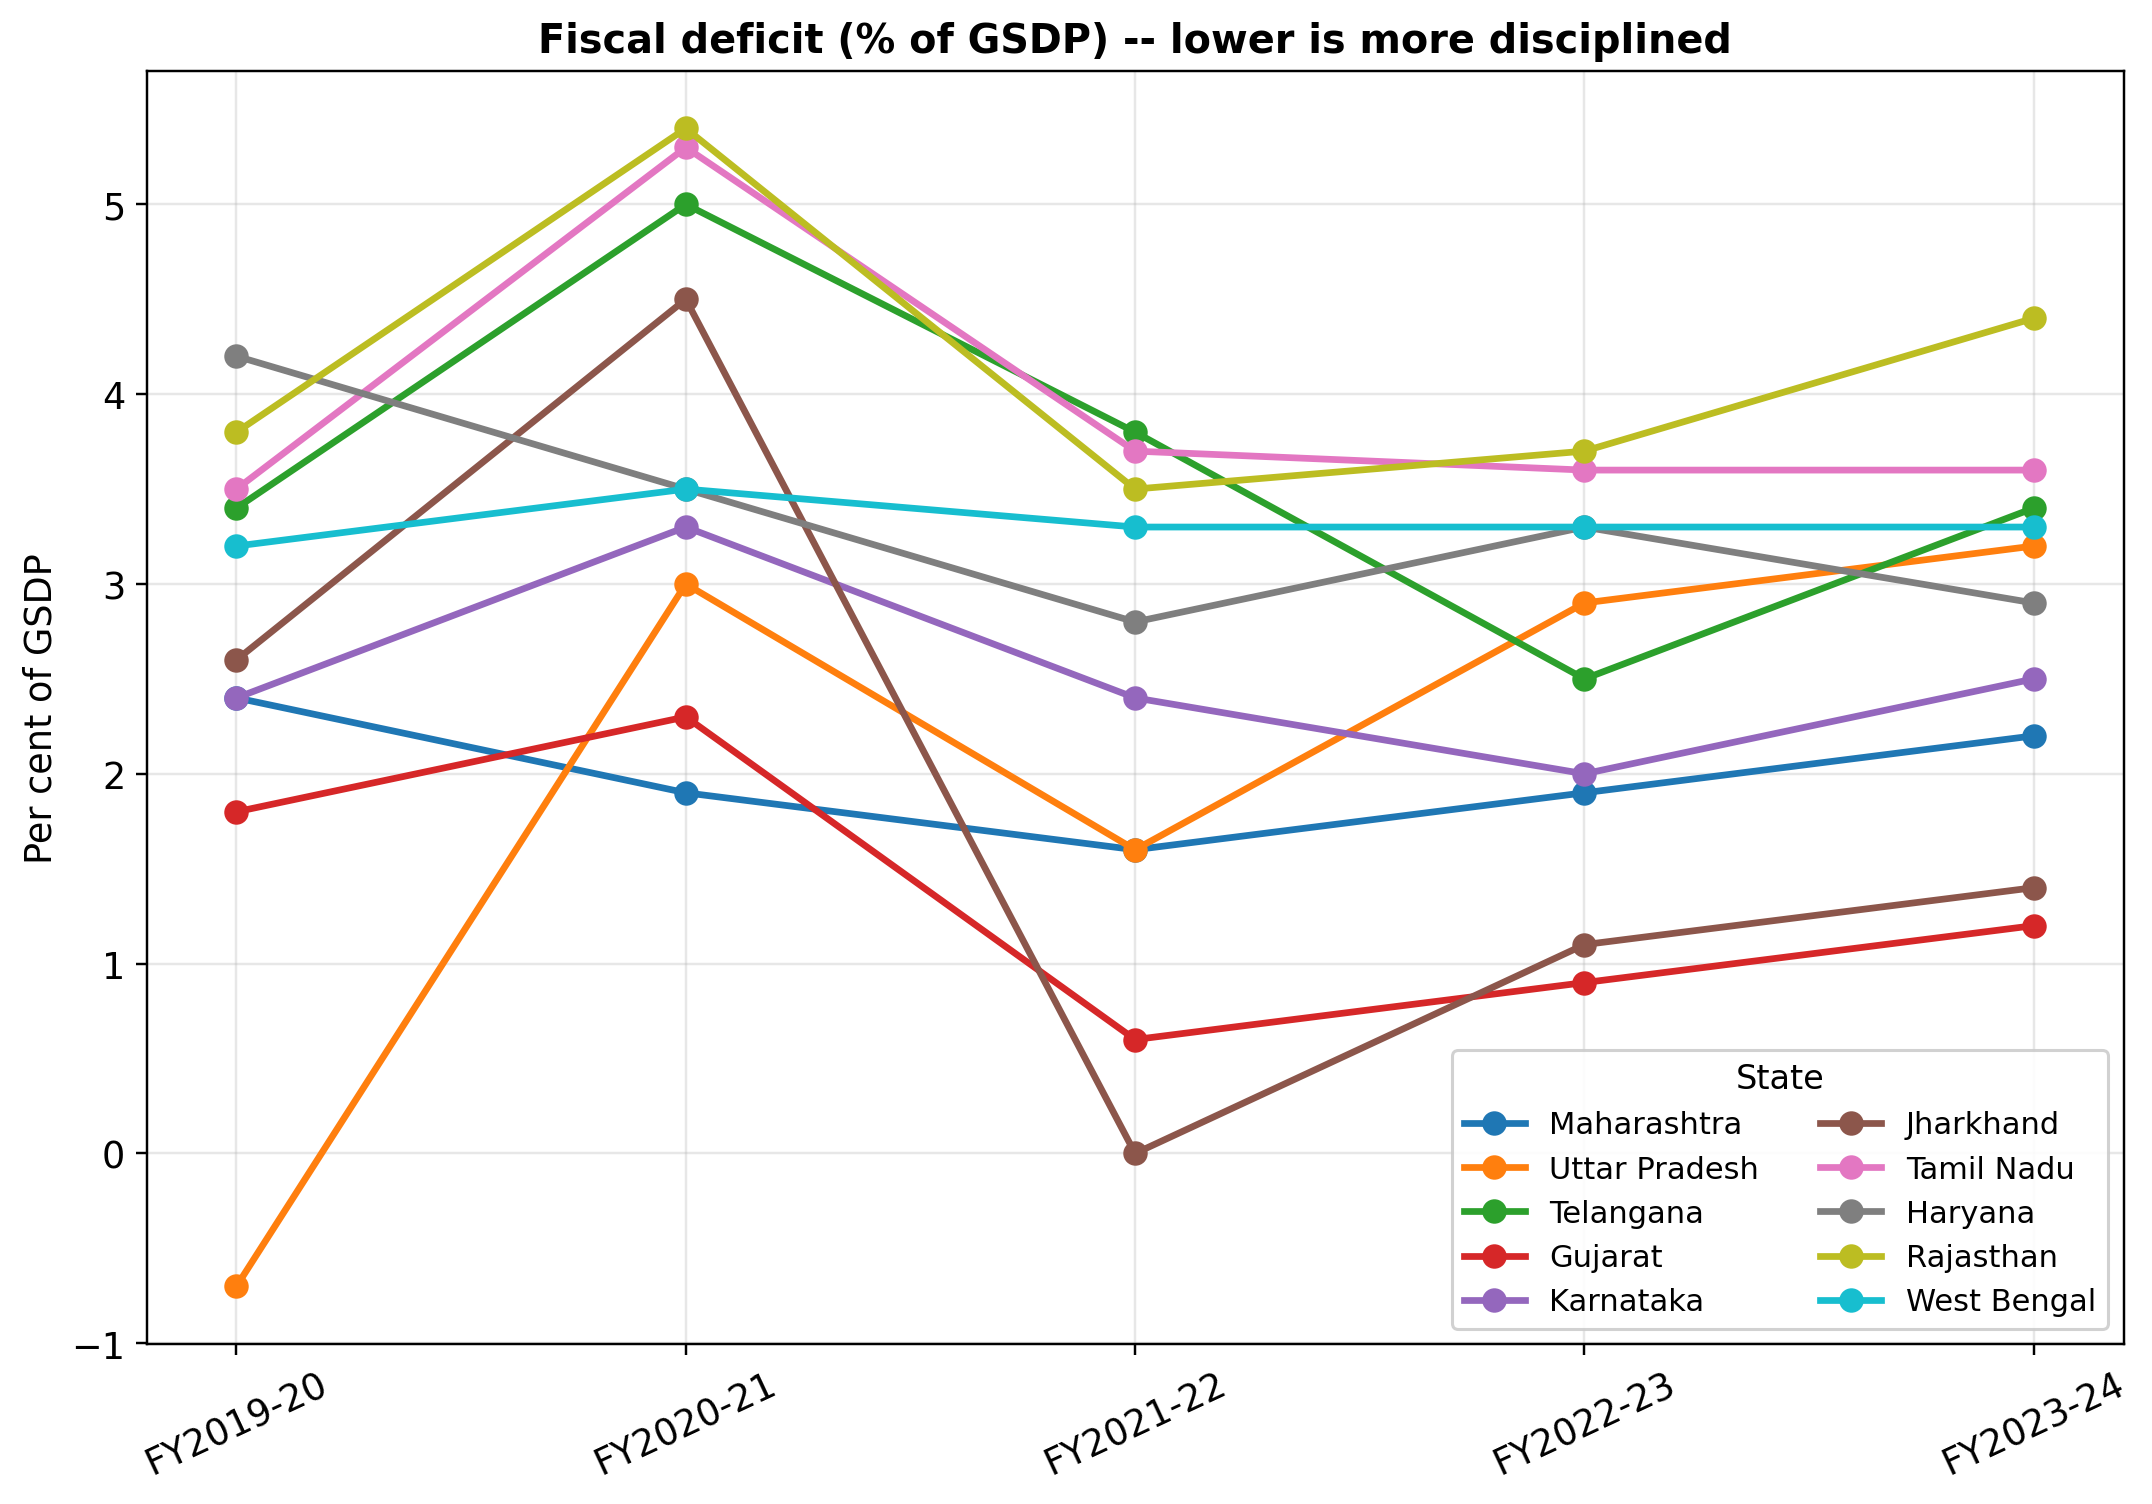
\includegraphics[width=0.82\textwidth]{figures/fig01.png}
\caption{Fiscal deficit, per cent of GSDP, FY 2019-20 to FY 2023-24, one line per state as shown in the legend. States with the flattest, lowest lines are the same states that rank best on fiscal discipline in Section 4.7.}
\label{fig:1}
\end{figure}

\begin{table}[H]
\centering
\caption{Outstanding liabilities (debt), Rupees crore, by state and fiscal year.}
\label{tab:3}
\footnotesize
\begin{adjustbox}{max width=\textwidth}
\begin{tabular}{@{}lrrrrrr@{}}
\toprule
State & FY2019-20 & FY2020-21 & FY2021-22 & FY2022-23 & FY2023-24 & 5-yr total \\
\midrule
Maharashtra & 486195 & 540405 & 584751 & 640912 & 730052 & 2982315 \\
Uttar Pradesh & 503230 & 559266 & 614412 & 666110 & 784934 & 3127952 \\
Telangana & 237525 & 281987 & 318120 & 354186 & 399081 & 1590899 \\
Gujarat & 370316 & 416954 & 422598 & 471528 & 499716 & 2181112 \\
Karnataka & 319928 & 385752 & 441116 & 494860 & 577936 & 2219592 \\
Jharkhand & 94331 & 107405 & 109445 & 115202 & 123394 & 549777 \\
Tamil Nadu & 430546 & 554311 & 623822 & 706053 & 804000 & 3118732 \\
Haryana & 219216 & 244248 & 266752 & 303103 & 331081 & 1364400 \\
Rajasthan & 358000 & 409196 & 456490 & 487486 & 576652 & 2287824 \\
West Bengal & 437446 & 485265 & 523705 & 585148 & 632476 & 2664040 \\
\bottomrule
\end{tabular}
\end{adjustbox}
\par\smallskip
{\footnotesize\raggedright Computed as (debt \% of GSDP / 100) x that year's GSDP.\par}
\end{table}

\begin{table}[H]
\centering
\caption{Outstanding liabilities (debt), per cent of GSDP, by state and fiscal year. This is the ratio used as a regressor in Sections 5-6.}
\label{tab:4}
\footnotesize
\begin{adjustbox}{max width=\textwidth}
\begin{tabular}{@{}lrrrrrr@{}}
\toprule
State & FY2019-20 & FY2020-21 & FY2021-22 & FY2022-23 & FY2023-24 & 5-yr avg \\
\midrule
Maharashtra & 18.3 & 20.7 & 18.6 & 17.6 & 18.0 & 18.64 \\
Uttar Pradesh & 29.6 & 34.0 & 31.1 & 29.5 & 29.7 & 30.78 \\
Telangana & 25.0 & 29.9 & 28.3 & 27.0 & 27.3 & 27.5 \\
Gujarat & 22.9 & 25.8 & 22.0 & 21.4 & 20.6 & 22.54 \\
Karnataka & 19.8 & 23.5 & 22.3 & 21.8 & 22.6 & 22.0 \\
Jharkhand & 30.4 & 36.2 & 29.1 & 27.6 & 26.5 & 29.96 \\
Tamil Nadu & 24.7 & 31.0 & 30.1 & 29.5 & 29.9 & 29.04 \\
Haryana & 29.7 & 33.5 & 30.7 & 30.8 & 30.5 & 31.04 \\
Rajasthan & 35.8 & 40.2 & 38.2 & 35.9 & 37.9 & 37.6 \\
West Bengal & 37.1 & 42.5 & 39.4 & 38.2 & 38.3 & 39.1 \\
\bottomrule
\end{tabular}
\end{adjustbox}
\par\smallskip
{\footnotesize\raggedright Source: FC-16 Report Vol II Annexure 5.3 (States' Finance Accounts - AUDITED ACTUALS).\par}
\end{table}

As with fiscal deficit, the figure below plots the debt ratio year-on-year for all ten states.

\begin{figure}[H]
\centering
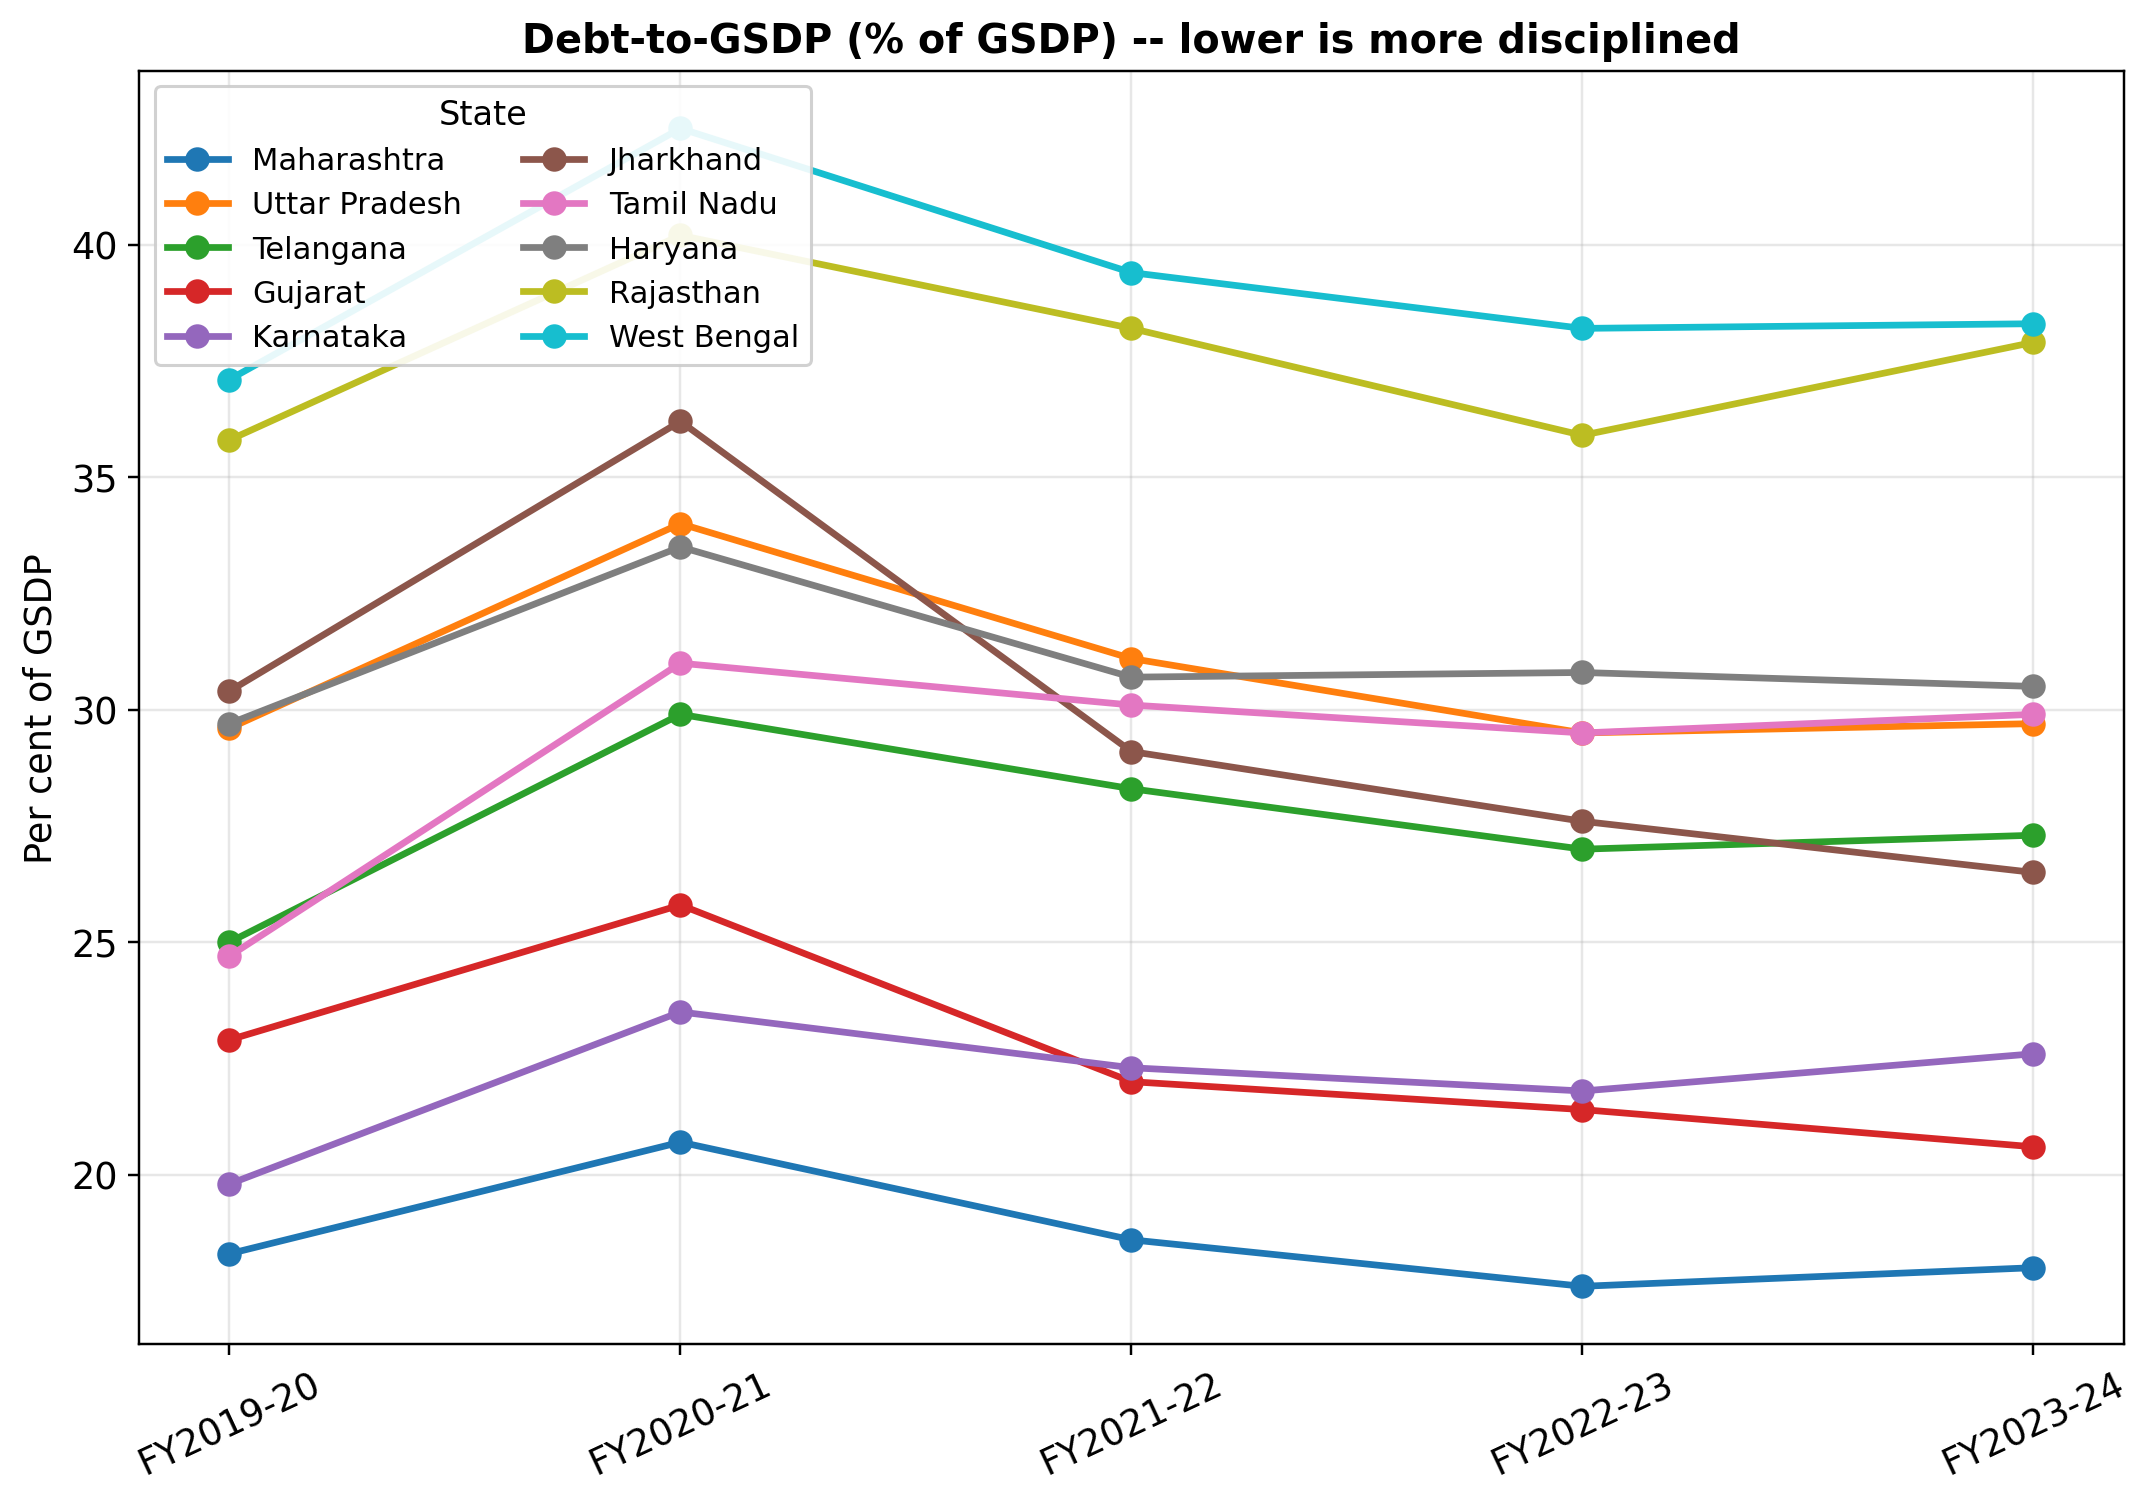
\includegraphics[width=0.82\textwidth]{figures/fig02.png}
\caption{Debt-to-GSDP, per cent of GSDP, FY 2019-20 to FY 2023-24, one line per state as shown in the legend. Gujarat and Maharashtra hold the lowest, flattest lines throughout; West Bengal and Rajasthan the highest.}
\label{fig:2}
\end{figure}

\begin{figure}[H]
\centering
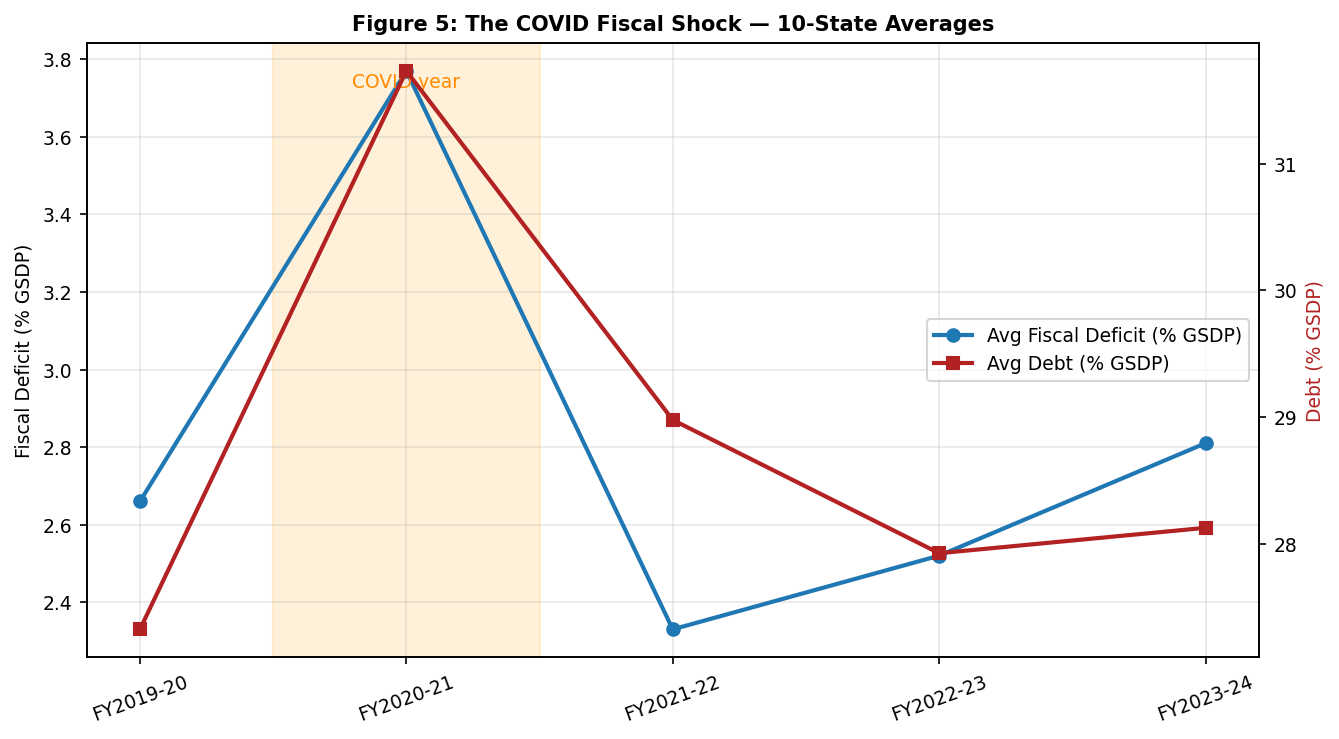
\includegraphics[width=1.00\textwidth]{figures/fig03.png}
\caption{The COVID-19 fiscal shock: ten-state average fiscal deficit and debt, FY 2019-20 to FY 2023-24. Both indicators deteriorate sharply in FY 2020-21 and partially recover thereafter; this shared shock is the reason the within-state and between-state regression coefficients in Section 6.3 point in different directions.}
\label{fig:3}
\end{figure}

\subsection{Own tax revenue, capital expenditure and revenue deficit, year-wise}
Own tax revenue captures how much a state raises on its own account rather than receiving from the centre. Capital expenditure captures spending that adds to the asset base. Revenue deficit, which is what remains when revenue expenditure runs ahead of revenue receipts, is carried here as an auxiliary series only, with a negative entry denoting a surplus; it is not one of the four regressors, but capital expenditure is derived from it. As in Section 4.3, each indicator appears first as a rupee amount and then as the percent-of-GSDP ratio the regressions use, followed by its year-wise trend chart.

\begin{table}[H]
\centering
\caption{Own tax revenue, Rupees crore, by state and fiscal year.}
\label{tab:5}
\footnotesize
\begin{adjustbox}{max width=\textwidth}
\begin{tabular}{@{}lrrrrrr@{}}
\toprule
State & FY2019-20 & FY2020-21 & FY2021-22 & FY2022-23 & FY2023-24 & 5-yr total \\
\midrule
Maharashtra & 191290 & 164471 & 223211 & 280399 & 300133 & 1159504 \\
Uttar Pradesh & 122407 & 120078 & 152121 & 178382 & 200859 & 773847 \\
Telangana & 68407 & 67903 & 92176 & 107568 & 112561 & 448615 \\
Gujarat & 92175 & 84037 & 115254 & 149831 & 162529 & 603826 \\
Karnataka & 101795 & 96848 & 120664 & 140740 & 161106 & 621153 \\
Jharkhand & 16756 & 16912 & 21438 & 25461 & 27938 & 108505 \\
Tamil Nadu & 109815 & 114438 & 128495 & 157964 & 177472 & 688184 \\
Haryana & 43548 & 43017 & 53872 & 64951 & 73815 & 279203 \\
Rajasthan & 60000 & 61074 & 75285 & 85548 & 97377 & 379284 \\
West Bengal & 61313 & 60515 & 70448 & 85781 & 89174 & 367231 \\
\bottomrule
\end{tabular}
\end{adjustbox}
\end{table}

\begin{table}[H]
\centering
\caption{Own tax revenue, per cent of GSDP, by state and fiscal year. This is the ratio used as a regressor in Sections 5-6.}
\label{tab:6}
\footnotesize
\begin{adjustbox}{max width=\textwidth}
\begin{tabular}{@{}lrrrrrr@{}}
\toprule
State & FY2019-20 & FY2020-21 & FY2021-22 & FY2022-23 & FY2023-24 & 5-yr avg \\
\midrule
Maharashtra & 7.2 & 6.3 & 7.1 & 7.7 & 7.4 & 7.14 \\
Uttar Pradesh & 7.2 & 7.3 & 7.7 & 7.9 & 7.6 & 7.54 \\
Telangana & 7.2 & 7.2 & 8.2 & 8.2 & 7.7 & 7.7 \\
Gujarat & 5.7 & 5.2 & 6.0 & 6.8 & 6.7 & 6.08 \\
Karnataka & 6.3 & 5.9 & 6.1 & 6.2 & 6.3 & 6.16 \\
Jharkhand & 5.4 & 5.7 & 5.7 & 6.1 & 6.0 & 5.78 \\
Tamil Nadu & 6.3 & 6.4 & 6.2 & 6.6 & 6.6 & 6.42 \\
Haryana & 5.9 & 5.9 & 6.2 & 6.6 & 6.8 & 6.28 \\
Rajasthan & 6.0 & 6.0 & 6.3 & 6.3 & 6.4 & 6.2 \\
West Bengal & 5.2 & 5.3 & 5.3 & 5.6 & 5.4 & 5.36 \\
\bottomrule
\end{tabular}
\end{adjustbox}
\par\smallskip
{\footnotesize\raggedright Source: FC-16 Report Vol II Annexure 5.5 (States' Finance Accounts - AUDITED ACTUALS).\par}
\end{table}

\begin{figure}[H]
\centering
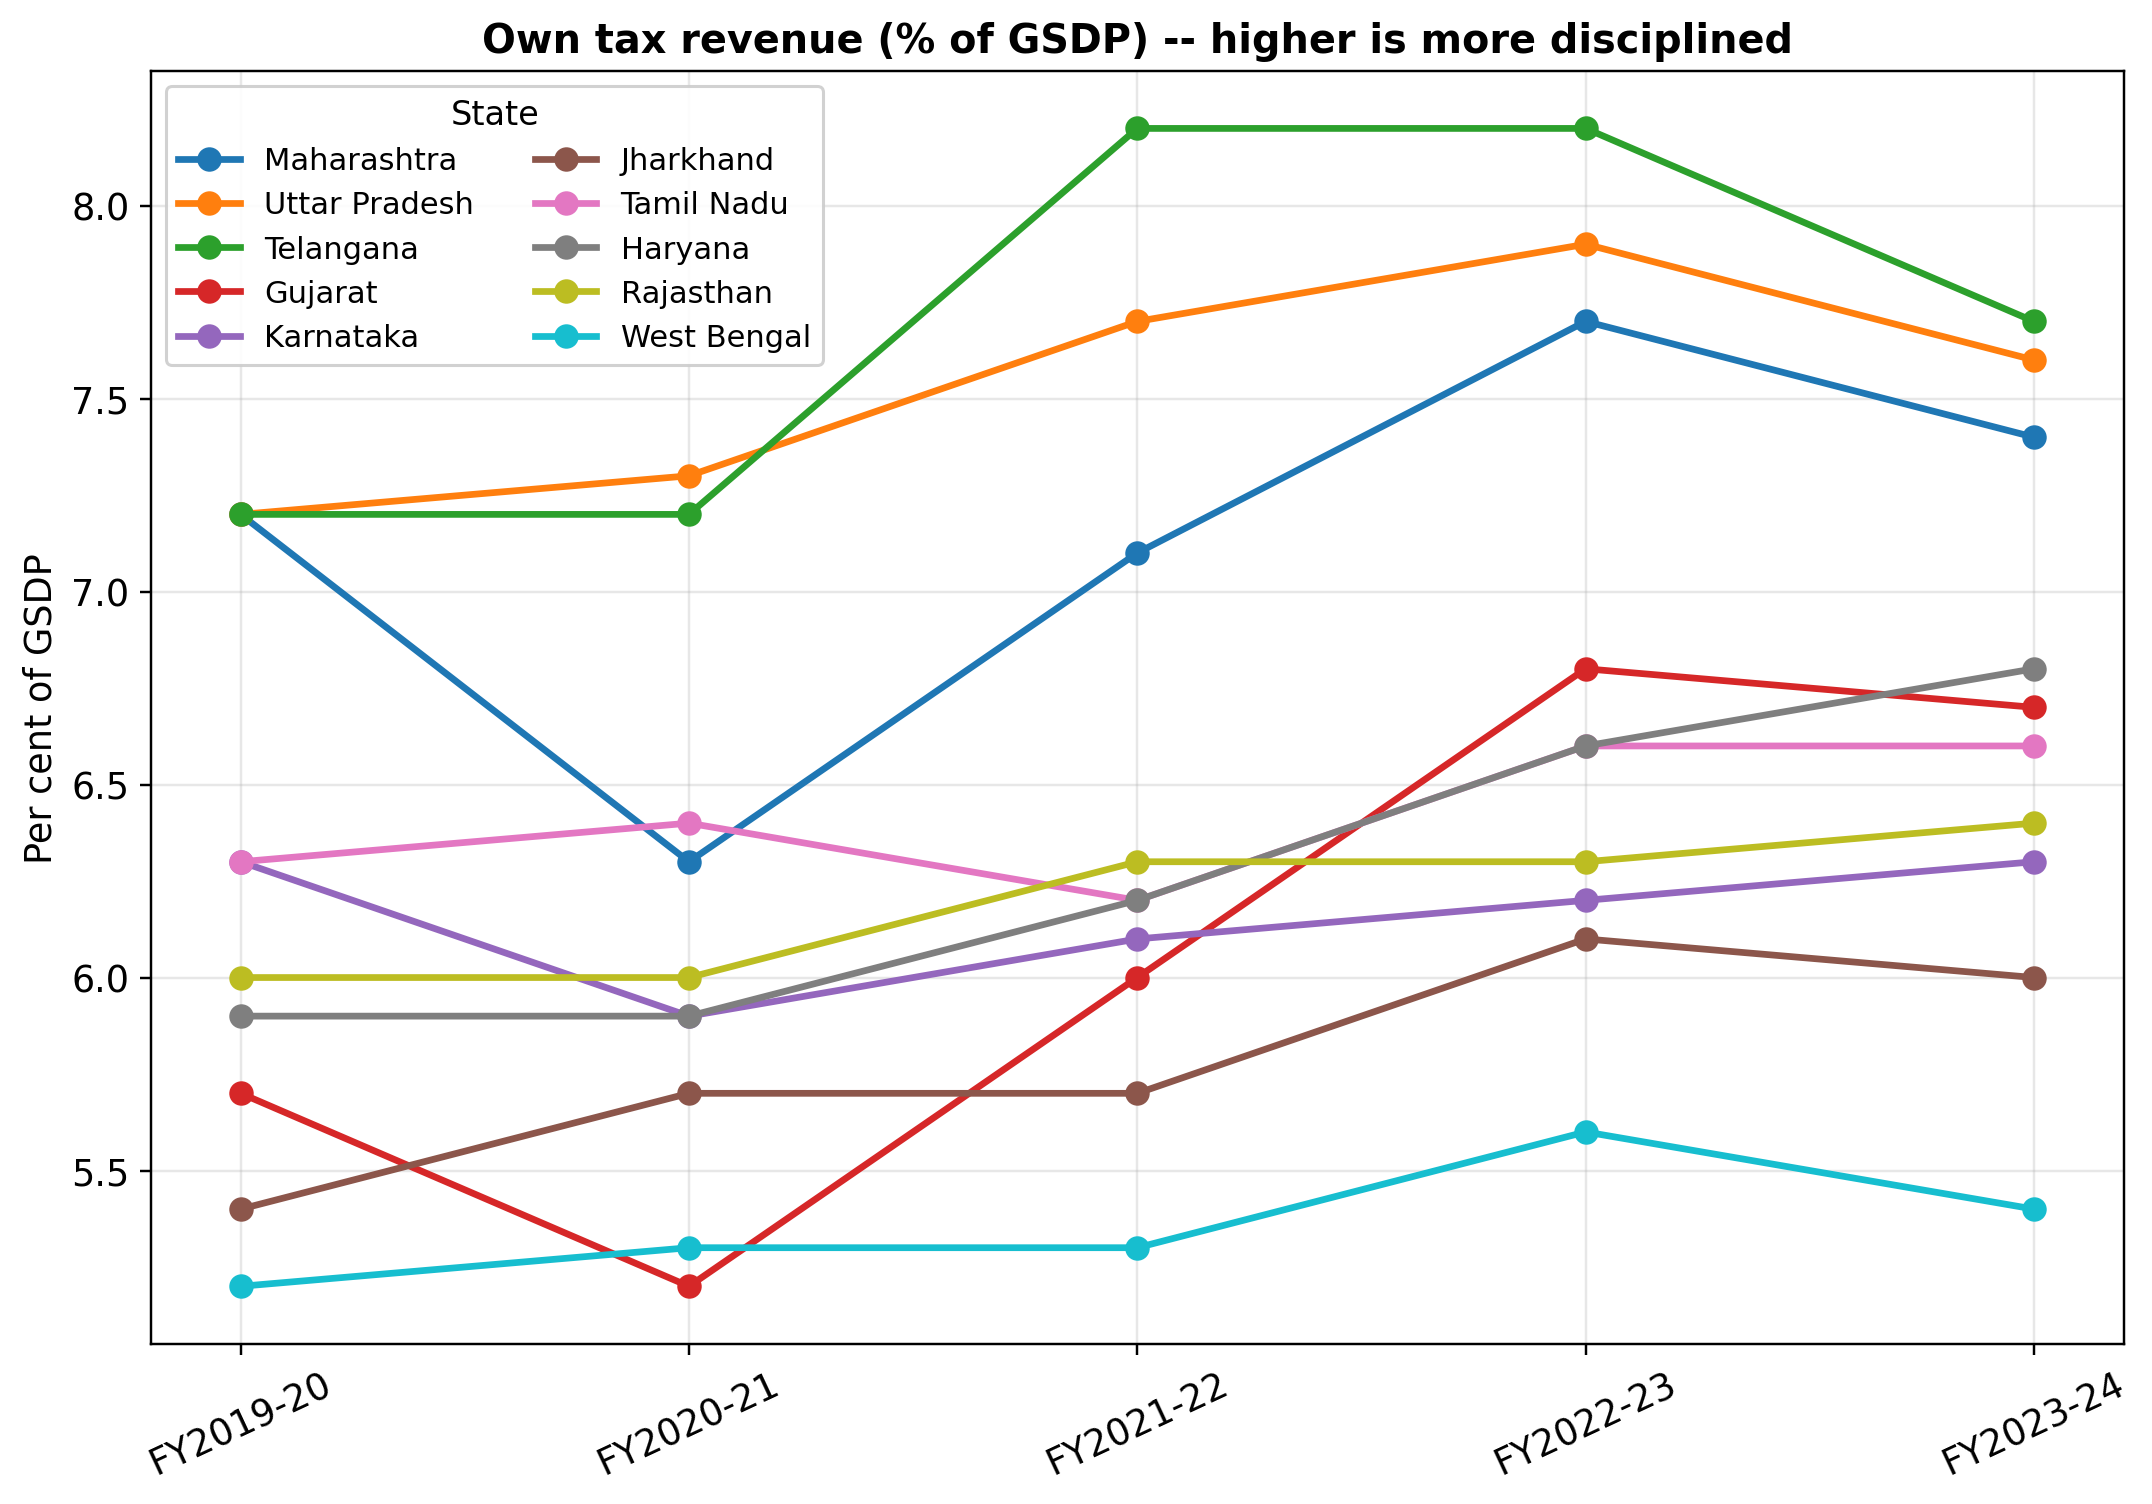
\includegraphics[width=0.82\textwidth]{figures/fig04.png}
\caption{Own tax revenue, per cent of GSDP, FY 2019-20 to FY 2023-24, one line per state as shown in the legend.}
\label{fig:4}
\end{figure}

\begin{table}[H]
\centering
\caption{Capital expenditure (derived), Rupees crore, by state and fiscal year.}
\label{tab:7}
\footnotesize
\begin{adjustbox}{max width=\textwidth}
\begin{tabular}{@{}lrrrrrr@{}}
\toprule
State & FY2019-20 & FY2020-21 & FY2021-22 & FY2022-23 & FY2023-24 & 5-yr total \\
\midrule
Maharashtra & 45166 & 20885 & 47157 & 65548 & 77061 & 255817 \\
Uttar Pradesh & 56103 & 52637 & 75073 & 103868 & 121572 & 409253 \\
Telangana & 25653 & 27350 & 38219 & 39354 & 51164 & 181740 \\
Gujarat & 30725 & 21009 & 34576 & 44068 & 70348 & 200726 \\
Karnataka & 40395 & 47604 & 51431 & 59020 & 53702 & 252152 \\
Jharkhand & 9930 & 11868 & 9402 & 18366 & 17694 & 67260 \\
Tamil Nadu & 24403 & 33974 & 37305 & 47868 & 48401 & 191951 \\
Haryana & 14024 & 7291 & 11296 & 14762 & 19539 & 66912 \\
Rajasthan & 1000 & 15268 & 22705 & 19011 & 27387 & 85371 \\
West Bengal & 17686 & 14843 & 18609 & 22977 & 28073 & 102188 \\
\bottomrule
\end{tabular}
\end{adjustbox}
\end{table}

\begin{table}[H]
\centering
\caption{Capital expenditure (derived), per cent of GSDP, by state and fiscal year, with cross-check capital-outlay figures for FY 2022-23 (actuals) and FY 2023-24 (revised estimates). This ratio is the regressor used in Sections 5-6.}
\label{tab:8}
\footnotesize
\begin{adjustbox}{max width=\textwidth}
\begin{tabular}{@{}lrrrrrrrr@{}}
\toprule
& \multicolumn{6}{c}{Derived capital expenditure (\% of GSDP)} & \multicolumn{2}{c}{Cross-check: capital outlay} \\
\cmidrule(lr){2-7}\cmidrule(lr){8-9}
State & FY2019-20 & FY2020-21 & FY2021-22 & FY2022-23 & FY2023-24 & 5-yr avg & FY2022-23 (A) & FY2023-24 (RE) \\
\midrule
Maharashtra & 1.7 & 0.8 & 1.5 & 1.8 & 1.9 & 1.54 & 1.69 & 2.12 \\
Uttar Pradesh & 3.3 & 3.2 & 3.8 & 4.6 & 4.6 & 3.9 & 4.12 & 6.19 \\
Telangana & 2.7 & 2.9 & 3.4 & 3.0 & 3.5 & 3.1 & 1.37 & 3.02 \\
Gujarat & 1.9 & 1.3 & 1.8 & 2.0 & 2.9 & 1.98 & 1.59 & 2.38 \\
Karnataka & 2.5 & 2.9 & 2.6 & 2.6 & 2.1 & 2.54 & 2.63 & 2.0 \\
Jharkhand & 3.2 & 4.0 & 2.5 & 4.4 & 3.8 & 3.58 & 3.56 & 5.06 \\
Tamil Nadu & 1.4 & 1.9 & 1.8 & 2.0 & 1.8 & 1.78 & 1.67 & 1.56 \\
Haryana & 1.9 & 1.0 & 1.3 & 1.5 & 1.8 & 1.5 & 1.19 & 1.32 \\
Rajasthan & 0.1 & 1.5 & 1.9 & 1.4 & 1.8 & 1.34 & 1.46 & 2.28 \\
West Bengal & 1.5 & 1.3 & 1.4 & 1.5 & 1.7 & 1.48 & 1.44 & 1.8 \\
\bottomrule
\end{tabular}
\end{adjustbox}
\par\smallskip
{\footnotesize\raggedright Derived: GFD minus RD (FC-16 Annex 5.1 - 5.2); includes net lending. Cross-check cols = exact capital outlay from state budget docs (Forum for State Studies) columns show exact capital outlay compiled from state budget documents, for comparison against the derived series.\par}
\end{table}

\begin{figure}[H]
\centering
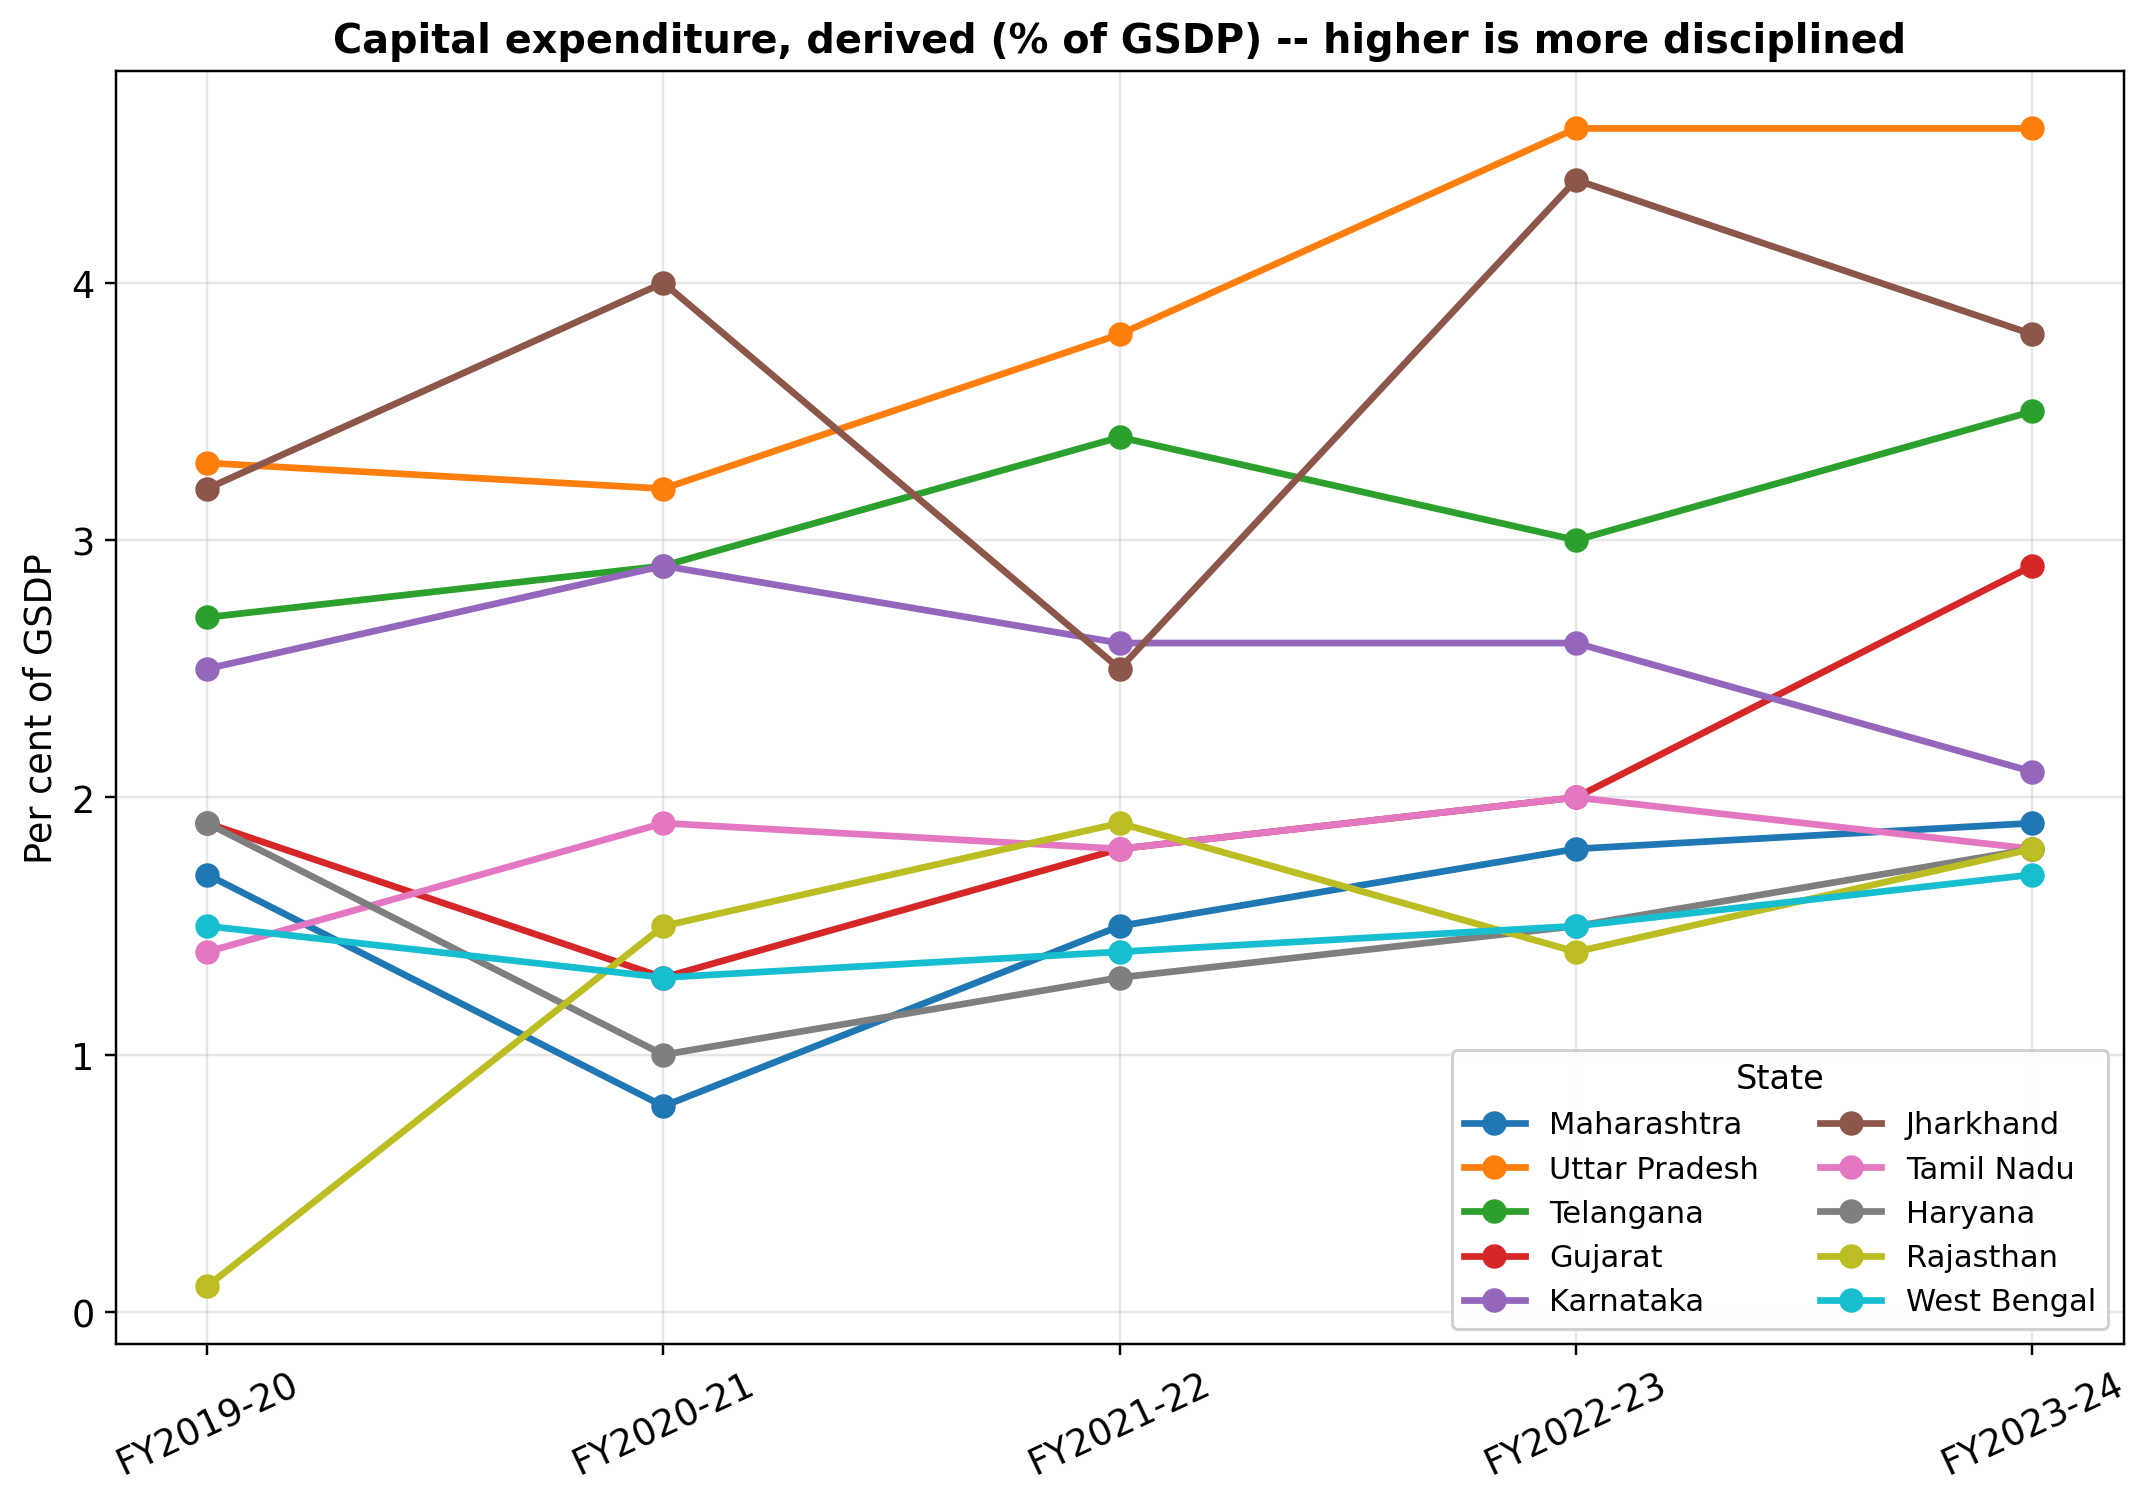
\includegraphics[width=0.82\textwidth]{figures/fig05.png}
\caption{Capital expenditure (derived), per cent of GSDP, FY 2019-20 to FY 2023-24, one line per state as shown in the legend.}
\label{fig:5}
\end{figure}

\begin{table}[H]
\centering
\caption{Revenue deficit, Rupees crore, by state and fiscal year.}
\label{tab:9}
\footnotesize
\begin{adjustbox}{max width=\textwidth}
\begin{tabular}{@{}lrrrrrr@{}}
\toprule
State & FY2019-20 & FY2020-21 & FY2021-22 & FY2022-23 & FY2023-24 & 5-yr total \\
\midrule
Maharashtra & 18598 & 28717 & 3144 & 3642 & 12168 & 66269 \\
Uttar Pradesh & -68004 & -3290 & -43463 & -38386 & -37000 & -190143 \\
Telangana & 6651 & 19805 & 4496 & -6559 & -1462 & 22931 \\
Gujarat & -1617 & 16161 & -23051 & -24237 & -41239 & -73983 \\
Karnataka & -1616 & 6566 & -3956 & -13620 & 10229 & -2397 \\
Jharkhand & -1862 & 1484 & -9402 & -13774 & -11175 & -34729 \\
Tamil Nadu & 36605 & 60795 & 39378 & 38294 & 48401 & 223473 \\
Haryana & 16976 & 18228 & 13034 & 17714 & 11941 & 77893 \\
Rajasthan & 37000 & 39698 & 19120 & 31232 & 39559 & 166609 \\
West Bengal & 20045 & 25120 & 25255 & 27572 & 26422 & 124414 \\
\bottomrule
\end{tabular}
\end{adjustbox}
\end{table}

\begin{table}[H]
\centering
\caption{Revenue deficit, per cent of GSDP, by state and fiscal year (negative = revenue surplus). Auxiliary variable; not used directly as a regressor, but is the series capital expenditure is derived from.}
\label{tab:10}
\footnotesize
\begin{adjustbox}{max width=\textwidth}
\begin{tabular}{@{}lrrrrrr@{}}
\toprule
State & FY2019-20 & FY2020-21 & FY2021-22 & FY2022-23 & FY2023-24 & 5-yr avg \\
\midrule
Maharashtra & 0.7 & 1.1 & 0.1 & 0.1 & 0.3 & 0.46 \\
Uttar Pradesh & -4.0 & -0.2 & -2.2 & -1.7 & -1.4 & -1.9 \\
Telangana & 0.7 & 2.1 & 0.4 & -0.5 & -0.1 & 0.52 \\
Gujarat & -0.1 & 1.0 & -1.2 & -1.1 & -1.7 & -0.62 \\
Karnataka & -0.1 & 0.4 & -0.2 & -0.6 & 0.4 & -0.02 \\
Jharkhand & -0.6 & 0.5 & -2.5 & -3.3 & -2.4 & -1.66 \\
Tamil Nadu & 2.1 & 3.4 & 1.9 & 1.6 & 1.8 & 2.16 \\
Haryana & 2.3 & 2.5 & 1.5 & 1.8 & 1.1 & 1.84 \\
Rajasthan & 3.7 & 3.9 & 1.6 & 2.3 & 2.6 & 2.82 \\
West Bengal & 1.7 & 2.2 & 1.9 & 1.8 & 1.6 & 1.84 \\
\bottomrule
\end{tabular}
\end{adjustbox}
\par\smallskip
{\footnotesize\raggedright Source: FC-16 Report Vol II Annexure 5.2 (negative = revenue surplus).\par}
\end{table}

\subsection{FDI and GSDP, year-wise}
FDI equity inflows by state are DPIIT's (2024) state-wise series, in Rupees crore, reported for the fiscal year in which the inflow was recorded. GSDP is the Ministry of Statistics and Programme Implementation's (MoSPI, 2024) state-wise series on the comparable 2011-12 base. GSDP growth is computed year-on-year from this series.

\begin{table}[H]
\centering
\caption{FDI equity inflows by state and fiscal year, Rupees crore.}
\label{tab:11}
\footnotesize
\begin{adjustbox}{max width=\textwidth}
\begin{tabular}{@{}lrrrrrr@{}}
\toprule
State & FY2019-20\textsuperscript{a} & FY2020-21 & FY2021-22 & FY2022-23 & FY2023-24 & Cumulative \\
\midrule
Maharashtra & 52073 & 119734 & 114964 & 118422 & 125101 & 532428.74 \\
Uttar Pradesh & NA (combined with FY2020-21; see note) & NA (combined with FY2019-20; see note) & 1619 & 3373 & 2762 & 12615.44 \\
Telangana & 4865 & 8618 & 11964 & 10319 & 25094 & 60860.43 \\
Gujarat & 18964 & 162830 & 20169 & 37059 & 60600 & 299624.37 \\
Karnataka & 30746 & 56884 & 163795 & 83628 & 54427 & 389483.39 \\
Jharkhand & 13208 & 5993 & 48 & 44 & 90 & 19382.14 \\
Tamil Nadu & 7230 & 17208 & 22396 & 17247 & 20157 & 84243.09 \\
Haryana & 5198 & 12559 & 20971 & 20735 & 15797 & 75269.59 \\
Rajasthan & 1347 & 2015 & 5277 & 7218 & 2195 & 18052.36 \\
West Bengal & 1363 & 3115 & 3195 & 3217 & 1501 & 12398.46 \\
\bottomrule
\end{tabular}
\end{adjustbox}
\end{table}

Source: DPIIT (2024). Uttar Pradesh's DPIIT state-wise reporting begins only in FY 2021-22; its FY 2019-20 and FY 2020-21 cells are not available separately and are treated as missing, not zero, throughout this paper. The cumulative column as originally published by DPIIT includes an unattributed combined figure for Uttar Pradesh's first two years and should not be summed against the state-year columns.

The first figure below totals this table by state; the second plots it year by year on a log scale so that both large states (Maharashtra, Karnataka) and small ones (Rajasthan, West Bengal) remain legible on the same axis.

\begin{figure}[H]
\centering
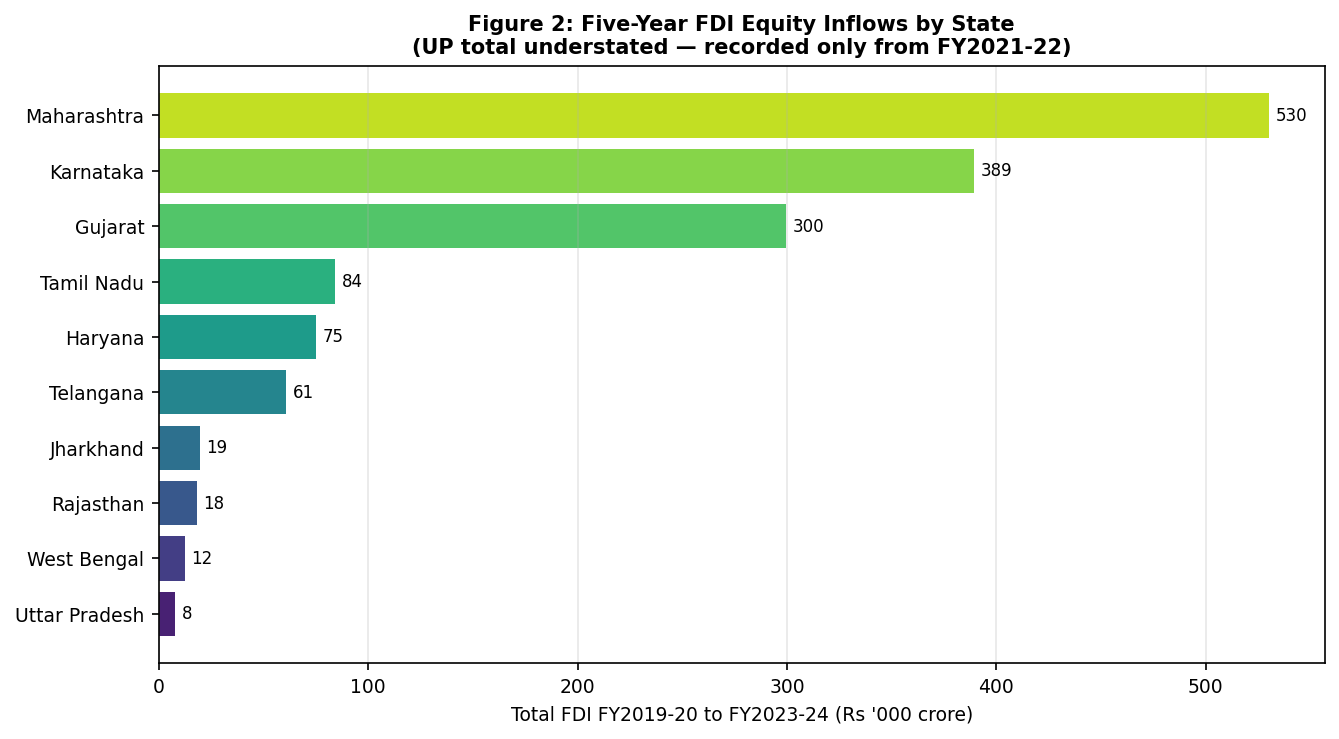
\includegraphics[width=1.00\textwidth]{figures/fig06.png}
\caption{Five-year total FDI equity inflows by state, FY 2019-20 to FY 2023-24. Uttar Pradesh's bar understates the state. DPIIT records its series only from FY 2021-22, so that bar is a floor, not a five-year total.}
\label{fig:6}
\end{figure}

\begin{figure}[H]
\centering
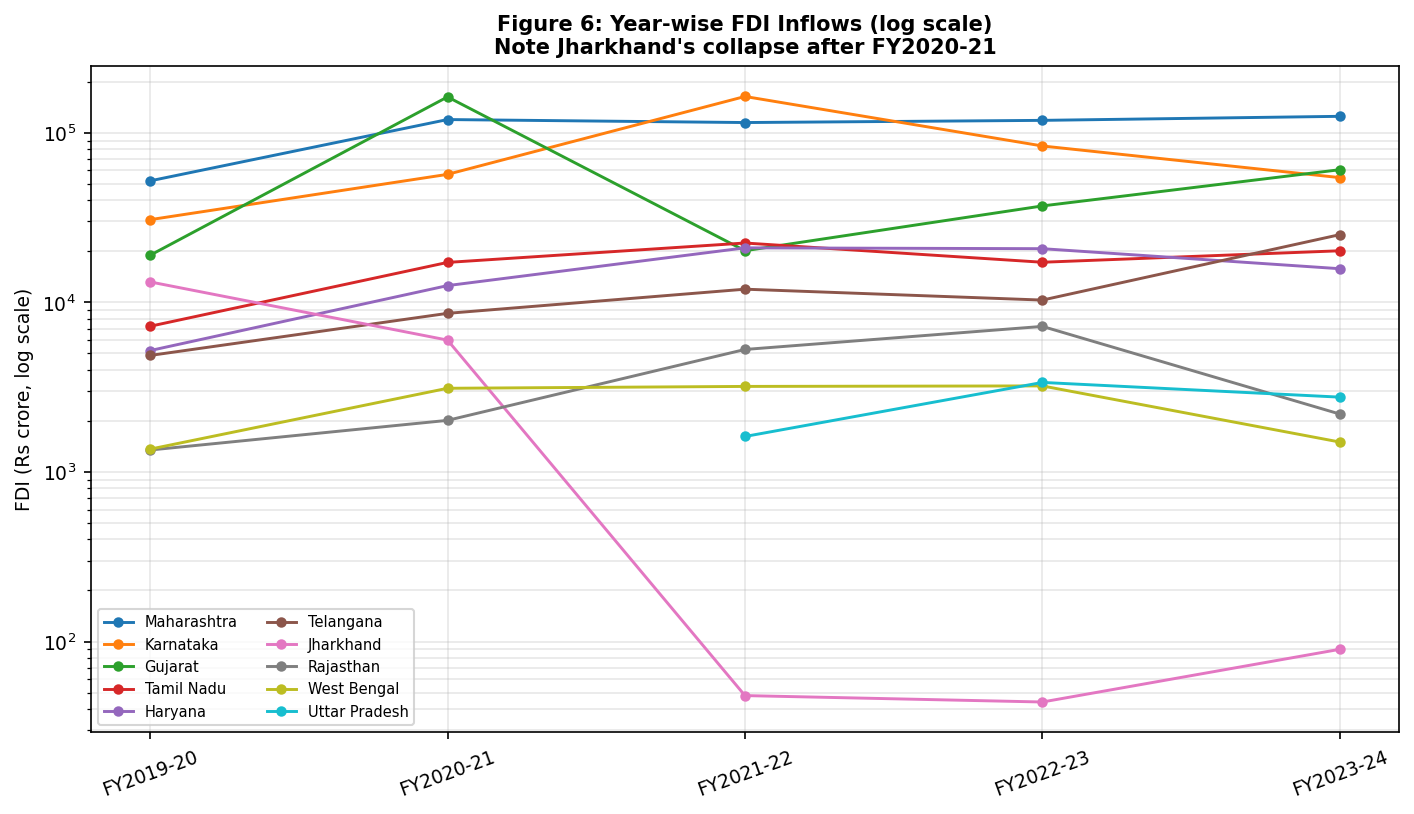
\includegraphics[width=0.99\textwidth]{figures/fig07.png}
\caption{Year-wise FDI inflows by state, log scale. Jharkhand's collapse after FY 2020-21 and Uttar Pradesh's left-censored early years are both visible here; the log scale is used because Maharashtra's FDI is roughly three orders of magnitude larger than Jharkhand's by FY 2023-24, which would compress every other state's line to a flat line on a linear axis.}
\label{fig:7}
\end{figure}

\begin{table}[H]
\centering
\caption{GSDP by state and fiscal year, Rupees crore.}
\label{tab:12}
\footnotesize
\begin{adjustbox}{max width=\textwidth}
\begin{tabular}{@{}lrrrrrr@{}}
\toprule
State & 2018-19 & 2019-20 & 2020-21 & 2021-22 & 2022-23 & 2023-24 \\
\midrule
Maharashtra & 2528854 & 2656806 & 2610651 & 3143821 & 3641543 & 4055847 \\
Uttar Pradesh & 1582200 & 1700100 & 1644900 & 1975600 & 2258000 & 2642877 \\
Telangana & 857400 & 950100 & 943100 & 1124100 & 1311800 & 1461836 \\
Gujarat & 1492200 & 1617100 & 1616100 & 1920900 & 2203400 & 2425804 \\
Karnataka & 1479400 & 1615800 & 1641500 & 1978100 & 2270000 & 2557241 \\
Jharkhand & 305700 & 310300 & 296700 & 376100 & 417400 & 465638 \\
Tamil Nadu & 1630200 & 1743100 & 1788100 & 2072500 & 2393400 & 2688963 \\
Haryana & 698900 & 738100 & 729100 & 868900 & 984100 & 1085510 \\
Rajasthan & 911500 & 1000000 & 1017900 & 1195000 & 1357900 & 1521510 \\
West Bengal & 1102100 & 1179100 & 1141800 & 1329200 & 1531800 & 1651374 \\
\bottomrule
\end{tabular}
\end{adjustbox}
\par\smallskip
{\footnotesize\raggedright Source: MoSPI (2024), 2011-12 comparable series.\par}
\end{table}

\begin{table}[H]
\centering
\caption{GSDP growth, per cent per annum, by state and fiscal year, computed year-on-year from the GSDP table above. This is the dependent variable in Model 2 (Section 5.1).}
\label{tab:13}
\footnotesize
\begin{adjustbox}{max width=\textwidth}
\begin{tabular}{@{}lrrrrrr@{}}
\toprule
State & FY2019-20 & FY2020-21 & FY2021-22 & FY2022-23 & FY2023-24 & 5-yr avg \\
\midrule
Maharashtra & 5.06 & -1.74 & 20.42 & 15.83 & 11.38 & 10.19 \\
Uttar Pradesh & 7.45 & -3.25 & 20.10 & 14.29 & 17.05 & 11.13 \\
Telangana & 10.81 & -0.74 & 19.19 & 16.70 & 11.44 & 11.48 \\
Gujarat & 8.37 & -0.06 & 18.86 & 14.71 & 10.09 & 10.39 \\
Karnataka & 9.22 & 1.59 & 20.51 & 14.76 & 12.65 & 11.75 \\
Jharkhand & 1.50 & -4.38 & 26.76 & 10.98 & 11.56 & 9.28 \\
Tamil Nadu & 6.93 & 2.58 & 15.91 & 15.48 & 12.35 & 10.65 \\
Haryana & 5.61 & -1.22 & 19.17 & 13.26 & 10.30 & 9.42 \\
Rajasthan & 9.71 & 1.79 & 17.40 & 13.63 & 12.05 & 10.92 \\
West Bengal & 6.99 & -3.16 & 16.41 & 15.24 & 7.81 & 8.66 \\
\bottomrule
\end{tabular}
\end{adjustbox}
\end{table}

\begin{figure}[H]
\centering
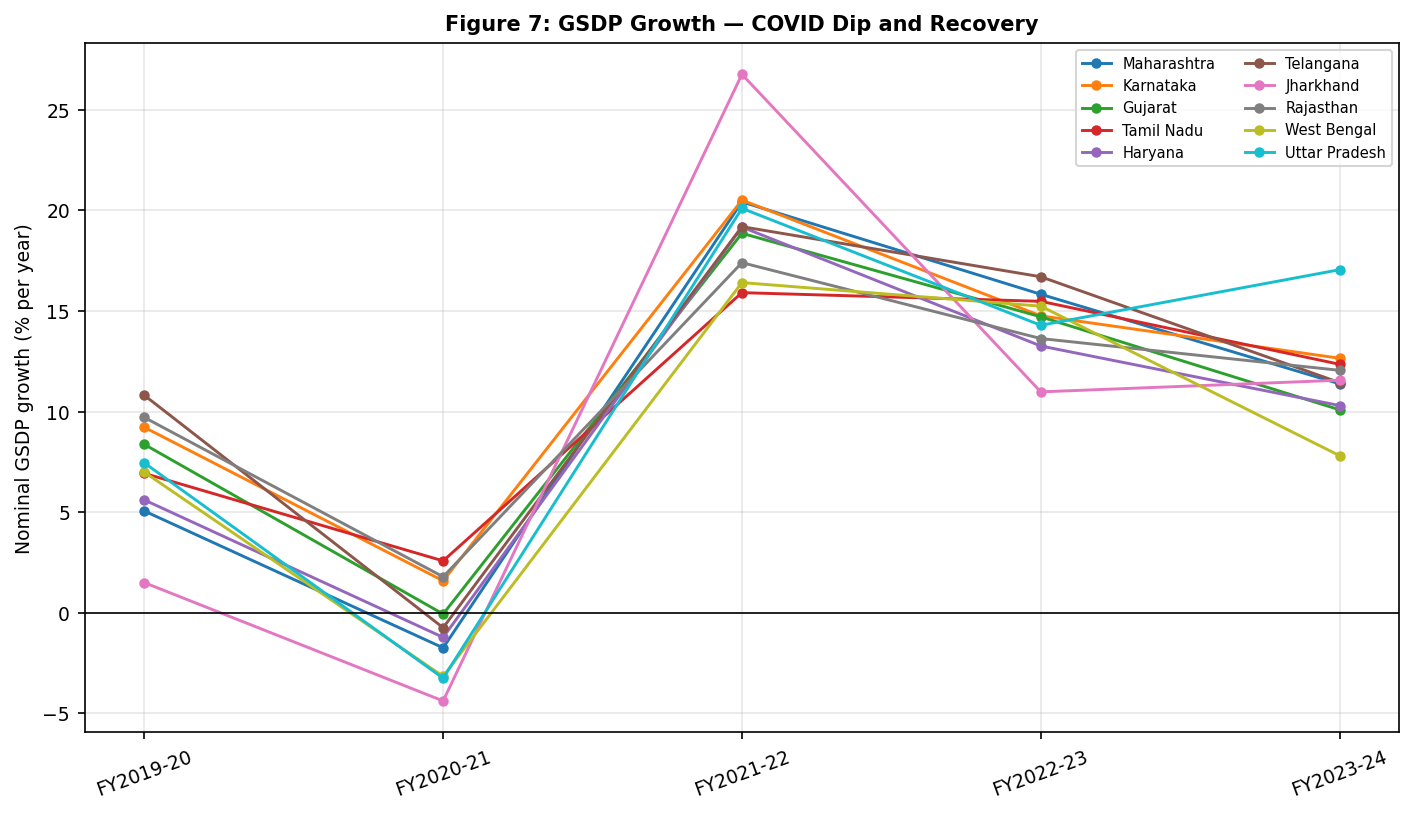
\includegraphics[width=0.99\textwidth]{figures/fig08.png}
\caption{GSDP growth by state, FY 2019-20 to FY 2023-24, showing the COVID-19 dip in FY 2020-21, common to all ten states, and the subsequent recovery.}
\label{fig:8}
\end{figure}

\subsection{Control variables}
Two controls enter only the pooled cross-state specification of Section 5.1, since the fixed-effects model already absorbs every time-invariant state characteristic by construction. They are the literacy rate and the urbanisation rate as recorded in the Primary Census Abstract of Census 2011 (Office of the Registrar General and Census Commissioner, India, 2011), which remains the latest full enumeration available.

\begin{table}[H]
\centering
\caption{Literacy and urbanisation rate by state, Census 2011.}
\label{tab:14}
\footnotesize
\begin{adjustbox}{max width=\textwidth}
\begin{tabular}{@{}lrrl@{}}
\toprule
State & Literacy (\%) & Urbanisation (\%) & Source \\
\midrule
Maharashtra & 82.3 & 45.2 & Census 2011 PCA \\
Uttar Pradesh & 67.7 & 22.3 & Census 2011 PCA \\
Telangana & 66.5 & 38.9 & Census 2011 PCA \\
Gujarat & 78 & 42.6 & Census 2011 PCA \\
Karnataka & 75.4 & 38.6 & Census 2011 PCA \\
Jharkhand & 66.4 & 24.1 & Census 2011 PCA \\
Tamil Nadu & 80.1 & 48.4 & Census 2011 PCA \\
Haryana & 75.6 & 34.9 & Census 2011 PCA \\
Rajasthan & 66.1 & 24.9 & Census 2011 PCA \\
West Bengal & 76.3 & 31.9 & Census 2011 PCA \\
\bottomrule
\end{tabular}
\end{adjustbox}
\end{table}

\begin{figure}[H]
\centering
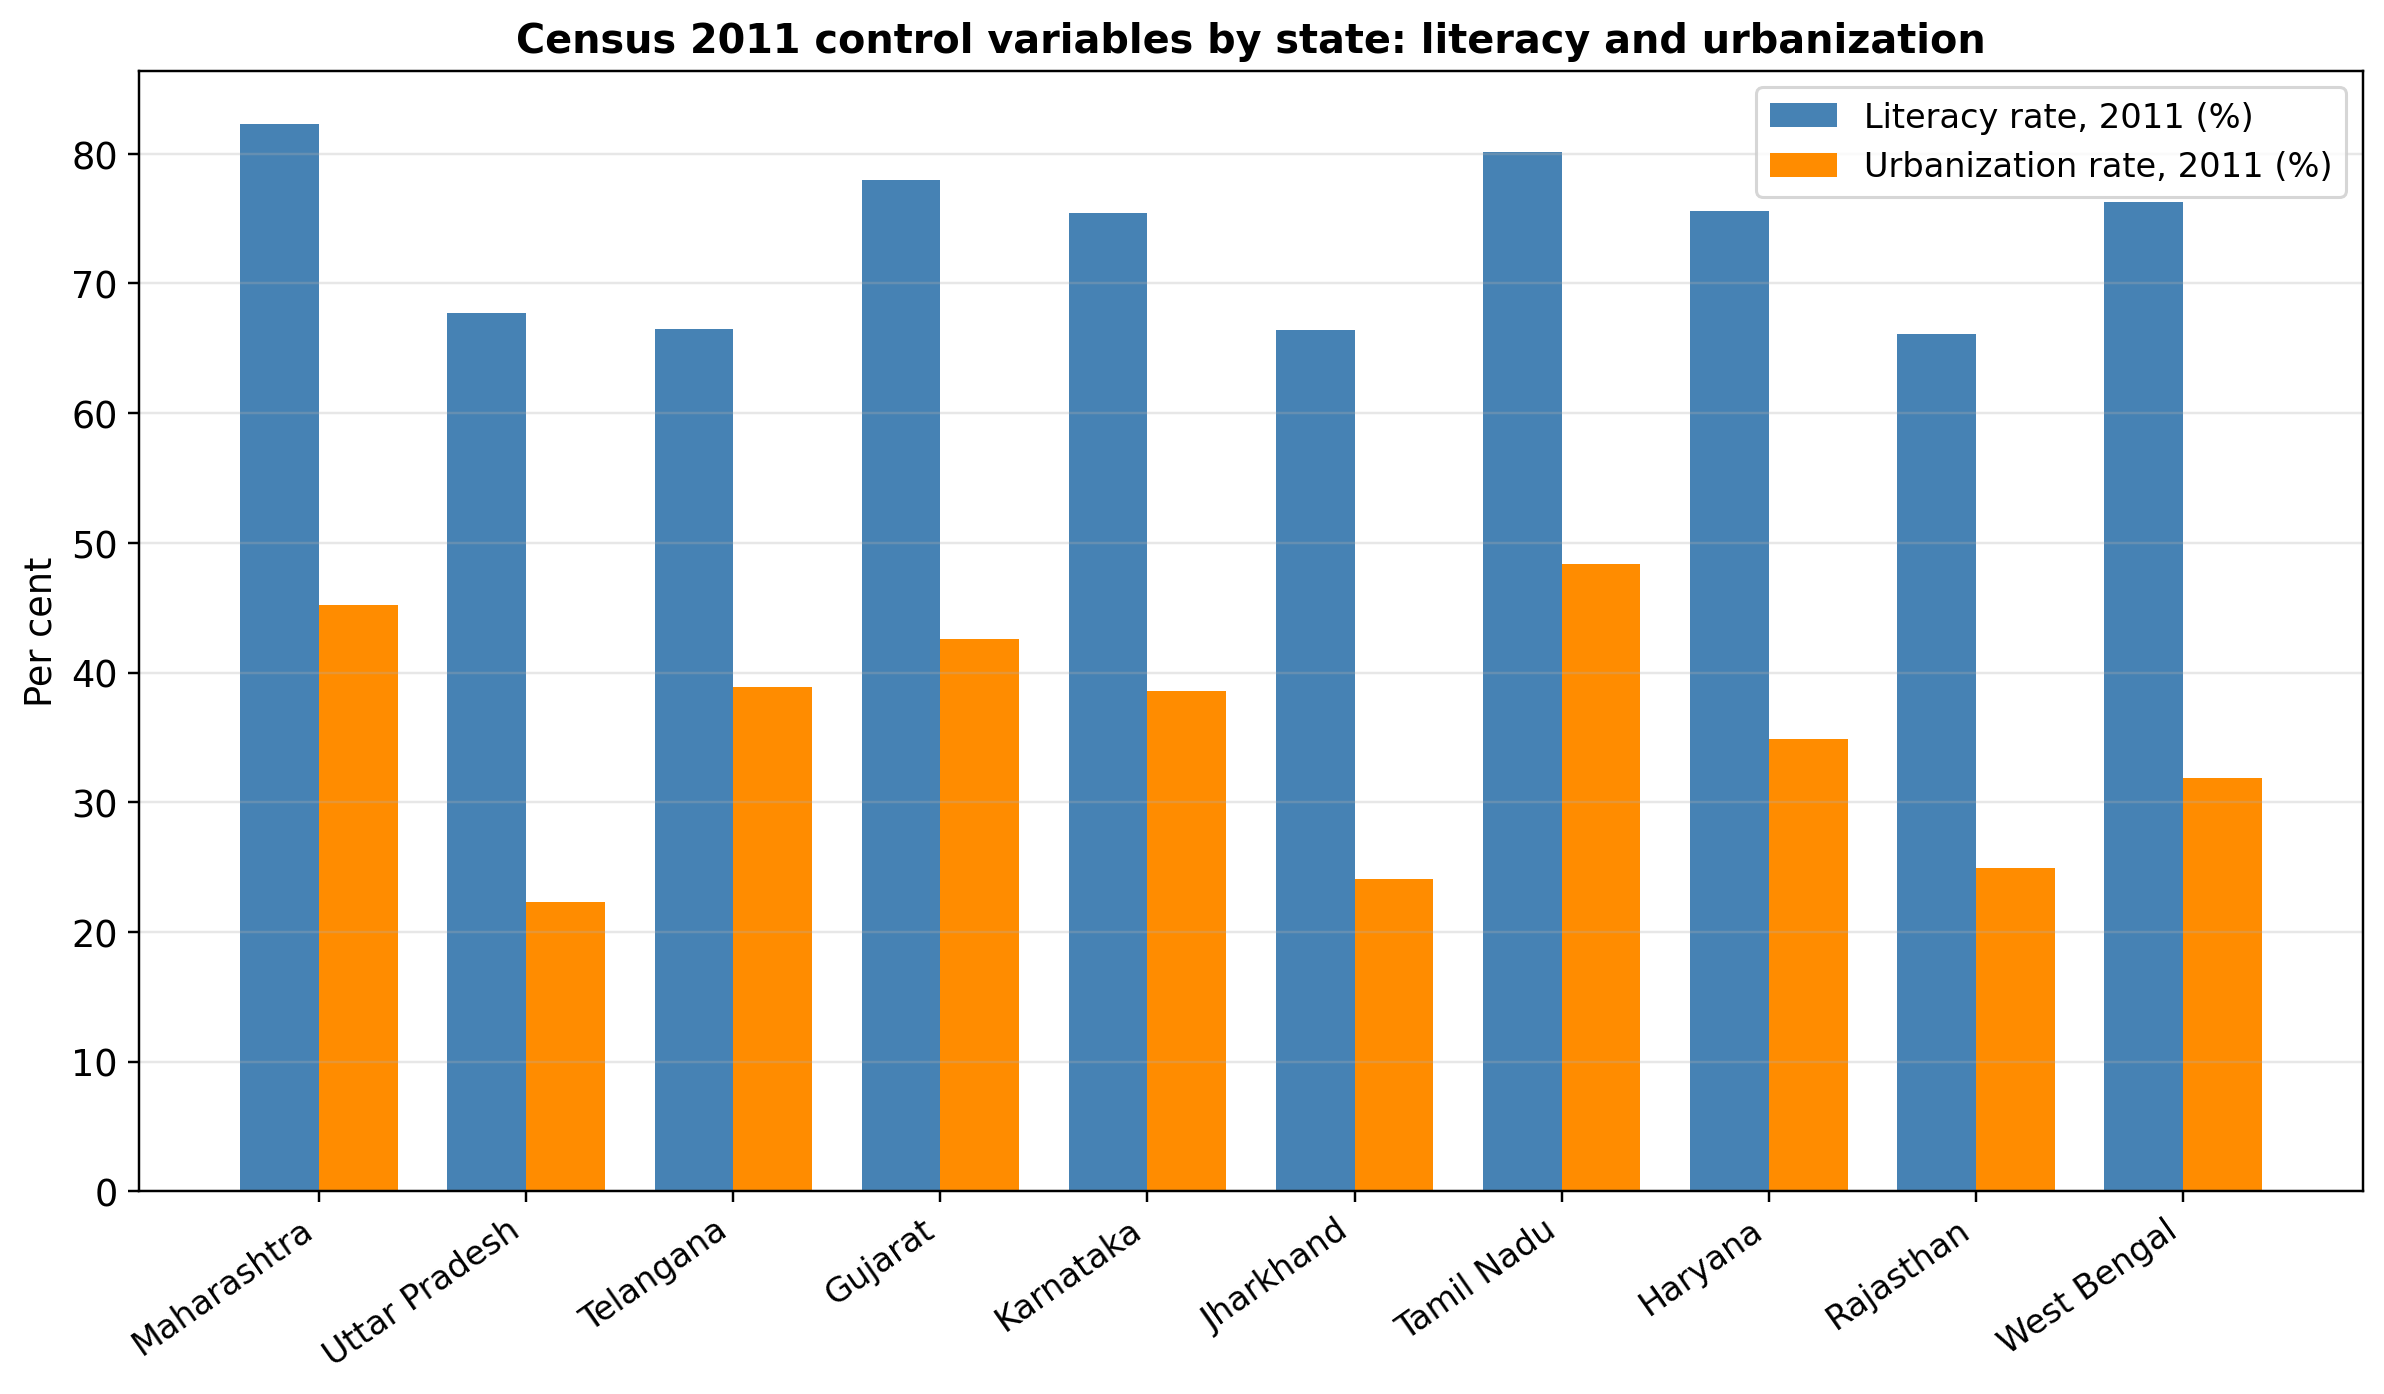
\includegraphics[width=0.98\textwidth]{figures/fig09.png}
\caption{Literacy and urbanisation rate by state, Census 2011. States are listed in the same order as the fiscal tables above for ease of comparison.}
\label{fig:9}
\end{figure}

\subsection{Fiscal discipline ranking: construction and a worked example}
The composite fiscal discipline ranking reported in Section 6.2 is built from the four fiscal regressors only (fiscal deficit, debt, own tax revenue and capital expenditure) and excludes the auxiliary revenue-deficit series. For a given year (or, for the five-year composite ranking, for each state's five-year average), each of the four indicators is separately ranked across the ten states from 1 (most disciplined on that indicator) to 10 (least disciplined): ascending rank on fiscal deficit and on debt, since lower is more disciplined for both, and descending rank on own tax revenue and on capital expenditure, since higher is more disciplined for both. Where two states are exactly tied on an indicator, both receive the average of the ranks they would otherwise have occupied. A state's composite score is the simple average of its four sub-indicator ranks, and states are then ranked 1 to 10 on that composite score, lower being more disciplined. The two tables below apply this procedure, first to the five-year state averages, then independently within each fiscal year; the year-wise version is the series plotted in the heatmap figure that follows the tables.

As a worked example, take Gujarat in FY 2022-23. Its fiscal deficit that year was 0.9 per cent of GSDP, the lowest of the ten states, giving it rank 1 on that indicator. Its debt was 21.4 per cent of GSDP, the second-lowest, giving rank 2. Its own tax revenue was 6.8 per cent of GSDP, the fourth-highest, giving rank 4. Its capital expenditure was 2.0 per cent of GSDP, tied for the fifth-highest with Tamil Nadu, giving both states a shared rank of 5.5. Gujarat's composite score for FY 2022-23 is therefore (1 + 2 + 4 + 5.5) / 4 = 3.125, the lowest (best) composite score of any state that year, which is why Gujarat is shown ranked first for FY 2022-23 in the year-wise ranking table and heatmap figure below.

\begin{table}[H]
\centering
\caption{Composite fiscal discipline ranking, five-year state averages (1 = most disciplined). Each state's rank on each of the four indicators (Rank columns) is computed from its own five-year average of that indicator, then the four ranks are averaged into the Composite Score column, and states are ordered by that score.}
\label{tab:15}
\footnotesize
\begin{adjustbox}{max width=\textwidth}
\begin{tabular}{@{}llrrrrrrrrr@{}}
\toprule
Rank & State & Composite\_Score(avg of 4 ranks; lower=more disciplined) & GFD avg & GFD rk & Debt avg & Debt rk & OTR avg & OTR rk & CapEx avg & CapEx rk \\
\midrule
1.0 & Uttar Pradesh & 3.375 & 2.0 & 3.5 & 30.78 & 7.0 & 7.54 & 2.0 & 3.9 & 1.0 \\
2.0 & Maharashtra & 3.625 & 2.0 & 3.5 & 18.64 & 1.0 & 7.14 & 3.0 & 1.54 & 7.0 \\
3.0 & Telangana & 4.0 & 3.62 & 8.0 & 27.5 & 4.0 & 7.7 & 1.0 & 3.1 & 3.0 \\
4.0 & Gujarat & 4.25 & 1.36 & 1.0 & 22.54 & 3.0 & 6.08 & 8.0 & 1.98 & 5.0 \\
5.0 & Karnataka & 4.5 & 2.52 & 5.0 & 22.0 & 2.0 & 6.16 & 7.0 & 2.54 & 4.0 \\
6.0 & Jharkhand & 4.75 & 1.92 & 2.0 & 29.96 & 6.0 & 5.78 & 9.0 & 3.58 & 2.0 \\
7.0 & Tamil Nadu & 6.0 & 3.94 & 9.0 & 29.04 & 5.0 & 6.42 & 4.0 & 1.78 & 6.0 \\
8.0 & Haryana & 7.0 & 3.34 & 7.0 & 31.04 & 8.0 & 6.28 & 5.0 & 1.5 & 8.0 \\
9.5 & Rajasthan & 8.75 & 4.16 & 10.0 & 37.6 & 9.0 & 6.2 & 6.0 & 1.34 & 10.0 \\
9.5 & West Bengal & 8.75 & 3.32 & 6.0 & 39.1 & 10.0 & 5.36 & 10.0 & 1.48 & 9.0 \\
\bottomrule
\end{tabular}
\end{adjustbox}
\par\smallskip
{\footnotesize\raggedright Composite score = simple average of the four sub-indicator ranks (fiscal deficit, debt, own tax revenue, capital expenditure); states are then ranked 1-10 on this score, with ties broken by the ranking algorithm and shown as shared rank numbers (e.g., Rajasthan and West Bengal both rank 9.5 on the underlying score, so both are listed at that position).\par}
\end{table}

\begin{table}[H]
\centering
\caption{Fiscal discipline rank by year (1 = most disciplined), computed independently for each fiscal year by the procedure worked through above, then averaged across the five years in the final column.}
\label{tab:16}
\footnotesize
\begin{adjustbox}{max width=\textwidth}
\begin{tabular}{@{}lrrrrrr@{}}
\toprule
State & FY2019-20 & FY2020-21 & FY2021-22 & FY2022-23 & FY2023-24 & 5-yr avg rank \\
\midrule
Maharashtra & 2 & 3 & 1 & 3 & 2 & 2.20 \\
Uttar Pradesh & 1 & 1 & 2 & 4 & 3 & 2.20 \\
Telangana & 4 & 4 & 3 & 2 & 4 & 3.40 \\
Gujarat & 5 & 5 & 5 & 1 & 1 & 3.40 \\
Karnataka & 3 & 2 & 4 & 6 & 6 & 4.20 \\
Jharkhand & 6 & 7 & 6 & 5 & 5 & 5.80 \\
Tamil Nadu & 7 & 6 & 8 & 7 & 8 & 7.20 \\
Haryana & 8 & 8 & 9 & 8 & 7 & 8.00 \\
Rajasthan & 9 & 9 & 7 & 9 & 9 & 8.60 \\
West Bengal & 10 & 10 & 10 & 10 & 10 & 10.00 \\
\bottomrule
\end{tabular}
\end{adjustbox}
\end{table}

\begin{figure}[H]
\centering
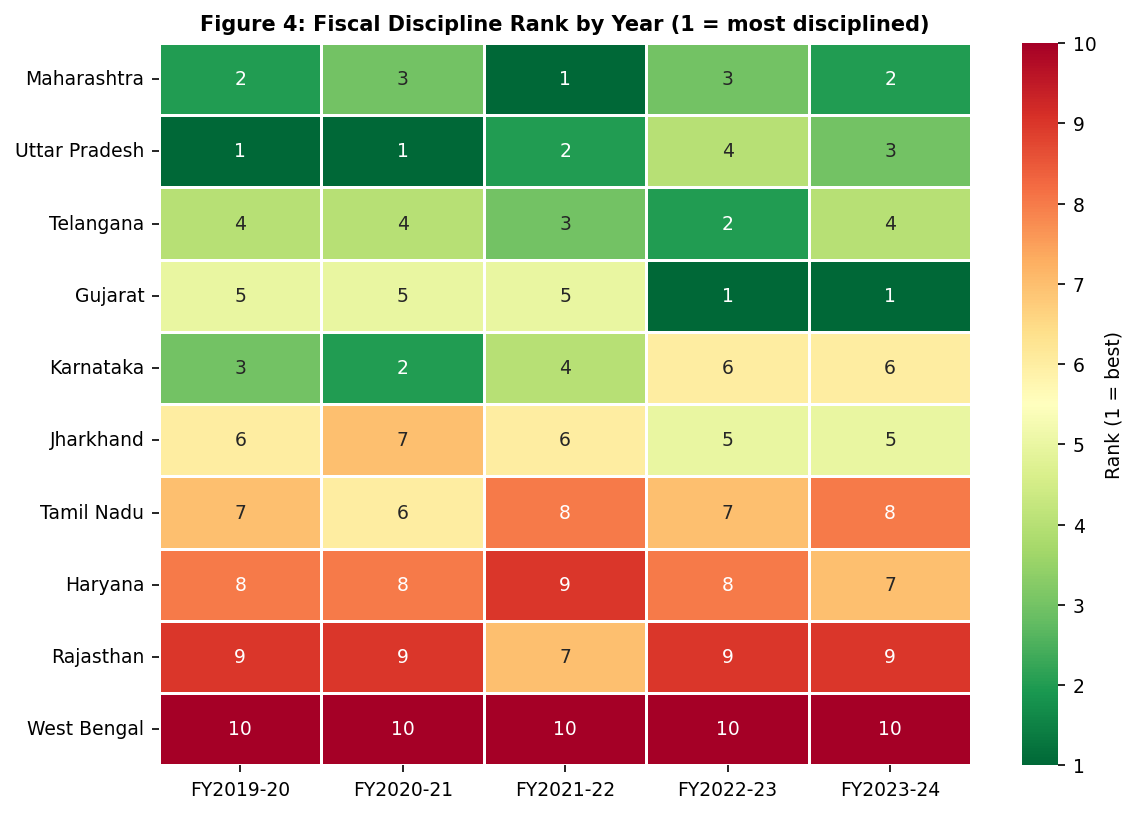
\includegraphics[width=0.80\textwidth]{figures/fig10.png}
\caption{Fiscal discipline rank by state and year, 1 (green) = most disciplined, 10 (red) = least disciplined. Each cell is one state-year's rank from Table 16 above; reading along a row shows whether a state's discipline improved, worsened, or stayed stable over the five years.}
\label{fig:10}
\end{figure}

Uttar Pradesh and Maharashtra share the best five-year average composite rank (2.2 in the year-wise average of Table 16; 3.375 and 3.625 respectively on the five-year-average composite score of Table 15, a slightly different number because Table 15 ranks the five-year mean of each indicator once, while Table 16 ranks each year separately and then averages the resulting yearly ranks). West Bengal is last on every single indicator combination in every single year of the panel, the only state with a perfect bottom-rank run.

\FloatBarrier
\section{Methodology}
\subsection{Econometric specification}
Two models are estimated, using the fiscal ratios (not the amounts) from Section 4 as regressors:

\begin{equation}
\ln(\mathrm{FDI})_{it} = \alpha_i + \beta_1 \mathrm{FD}_{it} + \beta_2 \mathrm{DEBT}_{it} + \beta_3 \mathrm{OTR}_{it} + \beta_4 \mathrm{CAPEX}_{it} + \beta_5 \mathrm{COVID}_{t} + \varepsilon_{it}
\end{equation}
\begin{equation}
\mathrm{GROWTH}_{it} = \alpha_i + \gamma_1 \mathrm{FD}_{it} + \gamma_2 \mathrm{DEBT}_{it} + \gamma_3 \mathrm{OTR}_{it} + \gamma_4 \mathrm{CAPEX}_{it} + \gamma_5 \mathrm{COVID}_{t} + \nu_{it}
\end{equation}
with i denoting the state and t the fiscal year. Each model is estimated twice. The first fit is an entity fixed-effects panel with Driscoll-Kraay standard errors, which stay valid under cross-sectional dependence and serially correlated errors in a panel of this length (Driscoll and Kraay, 1998); it identifies the within-state relationship. The second is a pooled OLS with the two Census controls added and errors clustered by state, and it identifies the between-state relationship. Variance inflation factors are computed for the four fiscal regressors, because deficit and debt are mechanically linked: a state's debt stock is the accumulation of its past deficits. Dynamic panel estimators of the Arellano-Bond family (1991) are deliberately avoided here. At N = 10 and T = 5 the instrument count in a standard difference or system GMM setup would approach or exceed the number of cross-sectional units, a configuration Roodman (2009) identifies as unreliable. As a descriptive complement to the two regressions, Spearman's rank correlation (Spearman, 1904) is computed between the composite discipline ranking of Section 4.7 and each state's five-year FDI total and per-capita GSDP. Unlike the regression coefficients, which exploit year-by-year variation, this compresses each state to a single point; it is reported in Section 6.2.

\subsection{Machine-learning validation}
Panel regression on ten states and five years rests on thirty-three to forty residual degrees of freedom, and one of the five years is dominated by a single, extreme, common shock. A single specification's p-value is thin support for a policy claim in that setting. The debt-FDI finding is therefore validated with three additional, methodologically independent lenses, all appropriate at this sample size:

(a) LASSO regression (Tibshirani, 1996) with leave-one-out cross-validated regularisation strength, which asks which regressors survive shrinkage rather than which cross a p < 0.05 threshold;

(b) Elastic Net (Zou and Hastie, 2005) as a cross-check on the LASSO selection, since the two penalise correlated regressors differently;

(c) A shallow random forest (Breiman, 2001) (1,000 trees, maximum depth 3, minimum leaf size 4; depth and leaf constraints were chosen specifically to prevent a forest with 48 training rows from memorising individual states) with SHAP (SHapley Additive exPlanations; Lundberg and Lee, 2017) values, which ranks predictors by their average marginal contribution to each individual prediction and can, unlike a linear model, in principle detect a non-linear or threshold effect.

All three are restricted to the same five time-varying regressors the fixed-effects econometric model uses: fiscal deficit, debt, own tax revenue, capital expenditure and the COVID dummy. That restriction was not the original choice. An initial SHAP run that also carried the two time-invariant Census controls ranked urbanisation as the most important predictor by a wide margin, at mean \textbar{}SHAP\textbar{} = 1.30 against 0.25 for debt, the next variable down. On inspection this turned out to be a known failure mode of tree-based models rather than a real urbanisation effect. Urbanisation is fixed within a state across all five years, so the random forest could treat it as a near-unique fingerprint for which state an observation came from, re-learning the state fixed effect through the back door instead of any fiscal or structural relationship. We report it rather than quietly drop it, because it is a useful caution for anyone applying tree-based importance measures to short panels with few entities. Part B is rerun with literacy and urbanisation excluded, and the Section 6.6 results come from that corrected specification. A leave-one-state-out stability check, ten refits each excluding one state, then tests whether the LASSO selection depends on any single state. Finally, leave-one-out cross-validated out-of-sample R-squared is computed for OLS, LASSO and the random forest, not to claim predictive power at forty-eight observations but to report honestly how much of it exists.

\subsection{Analytical architecture: from source data to final validation}
The paper does not estimate one model and report it. It runs a chain of eleven numbered stages in which two independent estimation branches, one classical and one machine-learning, are built from the same panel and then brought together at a single convergence test. The design exists because of the sample size. On fifty state-year cells no individual specification is worth much on its own, so a finding is only accepted here if it appears in both branches, with the same sign, after each branch has survived its own diagnostics. Figure 11 sets out the stages, and the paragraphs after it explain what each group of stages is for.

The chain runs: source ingestion, panel construction and composite ranking, then a split into Branch A (fixed effects and pooled OLS, with diagnostics and subsample perturbation) and Branch B (LASSO, Elastic Net, and a shallow random forest read through SHAP, with a leakage audit and a stability layer), and finally a convergence test across both branches followed by case analysis of whatever the chain cannot fit.

\begin{figure}[p]
\centering
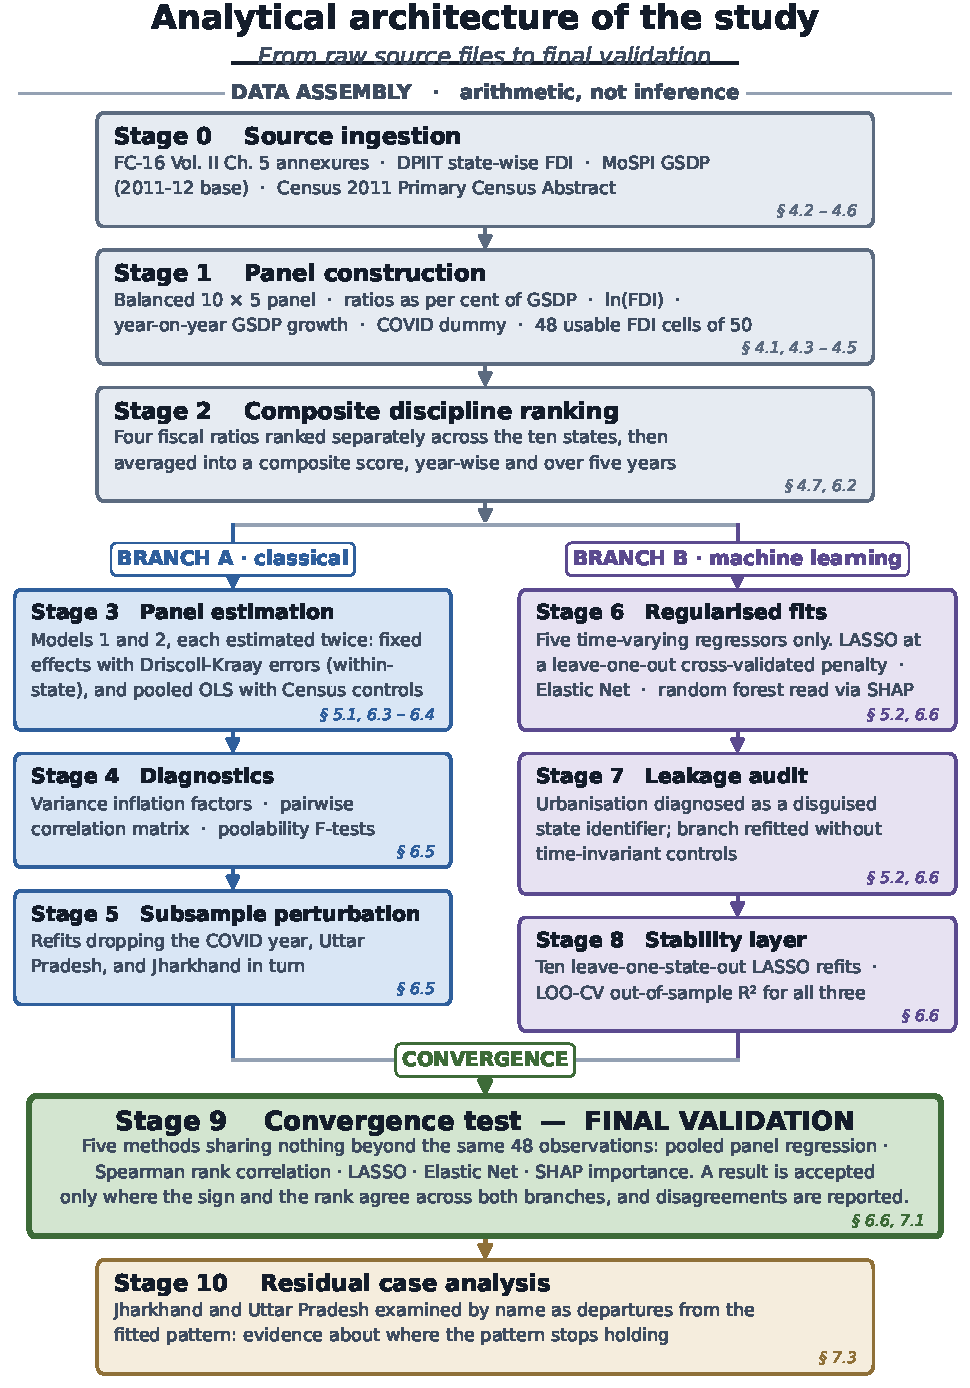
\includegraphics[width=\textwidth,keepaspectratio]{figures/fig_architecture.pdf}
\caption{Analytical architecture of the study, from raw source files to final validation. Boxes are numbered stages; the two vertical tracks are the classical and machine-learning estimation branches, which run in parallel on the same panel and meet at the Stage 9 convergence test.}
\label{fig:arch}
\end{figure}

Stages 0 to 2 are assembly, and they are arithmetic rather than inference. Everything in them is reproducible from the tables in Section 4. Three choices there propagate through the rest of the chain. Ratios are used instead of rupee amounts, because a rupee of deficit in Maharashtra and a rupee of deficit in Jharkhand are not comparable quantities. FDI enters in logs, because the largest recipient in the panel takes roughly three orders of magnitude more than the smallest in the same year. And the COVID dummy is created at this stage rather than being handled later, because FY 2020-21 is a shock common to all ten states; leaving it in the residual would contaminate every stage downstream of it.

Stages 3 to 5 are the classical branch. The two specifications are estimated in parallel, and neither is chosen over the other, because they identify different parameters. The fixed-effects fit uses only variation within a state across five years; the pooled fit is driven mostly by variation between states. Section 7.1 shows why keeping both was necessary, since they disagree on the sign of debt for a reason that is substantive rather than technical. Stages 4 and 5 are the branch auditing itself: whether the estimates depend on collinearity between deficit and debt, on the pandemic year, or on any one state.

Stages 6 to 8 are the machine-learning branch, and it is fed exactly the five time-varying regressors the fixed-effects model uses, no more. Stage 7 is where that restriction was decided rather than assumed, and it is reported because the failure it corrects is instructive. The first pass included the two Census controls and returned urbanisation as the dominant predictor by a factor of about five. Urbanisation is constant within a state across all five years, so the forest had found a near-unique fingerprint for state identity and was re-learning the fixed effect through the back door. Tree-based importance measures invite this on short panels with few entities, and a reader applying the same method elsewhere should expect it.

Stage 9 is the only stage that produces a conclusion, and it is what the whole architecture is built to reach. Five methods arrive at it: the pooled panel regression, the Spearman rank correlation, LASSO, Elastic Net, and SHAP importance from the random forest. They share nothing beyond the same forty-eight observations. Their distributional assumptions differ, their loss functions differ, and two of them are not hypothesis tests at all. Agreement among them on the sign and the rank of debt is accordingly much harder to obtain by chance than a single p-value below 0.05 would be, and exploiting that is the point of the design given how short the panel is. Where the five disagree, as they do on capital expenditure, the paper reports the disagreement and explains it (Section 7.2) rather than taking a majority verdict.

Stage 10 handles what the chain cannot fit. Two states break the pattern, and Section 7.3 treats them by name, as evidence about where the pattern stops holding rather than as noise to be absorbed into a residual.

\FloatBarrier
\section{Results}
\subsection{Descriptive statistics}
Before the regressions, a range check. The table gives the mean, dispersion and extremes of every fiscal ratio and outcome variable across the state-year observations, so that an implausible value would be visible before it entered a model. Nothing in it is a finding. Sample sizes differ: the four fiscal regressors and GSDP growth carry all fifty cells, while FDI and log FDI carry forty-eight, the two Uttar Pradesh gaps of Section 4.5.

\begin{table}[H]
\centering
\caption{Descriptive statistics for the panel (N = 50; FDI and log FDI, N = 48).}
\label{tab:17}
\footnotesize
\begin{adjustbox}{max width=\textwidth}
\begin{tabular}{@{}lrrrrrr@{}}
\toprule
 & $N$ & Mean & Std dev & Min & Median & Max \\
\midrule
Fiscal deficit (\% GSDP) & 50.0 & 2.82 & 1.26 & -0.7 & 3.1 & 5.4 \\
Debt (\% GSDP) & 50.0 & 28.82 & 6.55 & 17.6 & 29.55 & 42.5 \\
Own tax revenue (\% GSDP) & 50.0 & 6.47 & 0.8 & 5.2 & 6.3 & 8.2 \\
Capital expenditure (\% GSDP) & 50.0 & 2.27 & 1.01 & 0.1 & 1.9 & 4.6 \\
Revenue deficit (\% GSDP) & 50.0 & 0.54 & 1.77 & -4.0 & 0.6 & 3.9 \\
FDI (Rs crore) & 48.0 & 31194.46 & 43932.66 & 44.0 & 12883.5 & 163795.0 \\
GSDP growth (\%) & 50.0 & 10.39 & 7.35 & -4.38 & 11.41 & 26.76 \\
\bottomrule
\end{tabular}
\end{adjustbox}
\end{table}

One number in that table does foreshadow what follows. Debt-to-GSDP runs from 17.6 to 42.5 per cent across the panel. A fourteen-point spread over ten states is wide relative to the mean, and it is not scattered randomly. West Bengal and Rajasthan hold the top of the range in every year; Gujarat and Maharashtra hold the bottom. That ordering reappears in every result reported below.

\subsection{Fiscal discipline ranking and its relationship to outcomes}
Table 18 places each state's composite discipline rank from Section 4.7 next to its five-year FDI total and its FY 2023-24 per-capita GSDP, with the corresponding ranks and the Spearman correlations specified in Section 5.1. The question here is narrower than the one the regressions answer. It is not whether a state's FDI moves when its own fiscal position moves. It is whether the states that rank well on discipline across the whole window are the same states that end up with the most investment and the highest incomes.

\begin{table}[H]
\centering
\caption{Fiscal discipline composite rank against FDI and per-capita GSDP, with rank correlations.}
\label{tab:18}
\footnotesize
\begin{adjustbox}{max width=\textwidth}
\begin{tabular}{@{}lrrrrr@{}}
\toprule
State & Fiscal\_Discipline\_Composite\_Rank & FDI 5-yr total & FDI rank & Per-capita GSDP & PC GSDP rank \\
\midrule
Maharashtra & 2.0 & 530294.0 & 1.0 & 319474.0 & 6.0 \\
Karnataka & 5.0 & 389480.0 & 2.0 & 376402.0 & 2.0 \\
Gujarat & 4.0 & 299622.0 & 3.0 & 336875.0 & 5.0 \\
Tamil Nadu & 7.0 & 84238.0 & 4.0 & 349248.0 & 4.0 \\
Haryana & 8.0 & 75260.0 & 5.0 & 356829.0 & 3.0 \\
Telangana & 3.0 & 60860.0 & 6.0 & 382870.0 & 1.0 \\
Jharkhand & 6.0 & 19383.0 & 7.0 & 117124.0 & 9.0 \\
Rajasthan & 9.5 & 18052.0 & 8.0 & 186610.0 & 7.0 \\
West Bengal & 9.5 & 12391.0 & 9.0 & 166196.0 & 8.0 \\
Uttar Pradesh & 1.0 & 7754.0 & 10.0 & 111475.0 & 10.0 \\
\bottomrule
\end{tabular}
\end{adjustbox}
\end{table}

Spearman rank correlations: Discipline vs FDI (n=10): rho=0.255 p=0.476; Discipline vs PerCapita GSDP (n=10): rho=0.012 p=0.973; Discipline vs FDI excluding UP (n=9; UP FDI left-censored from FY22): rho=0.728 p=0.026; Discipline vs PerCapita GSDP excluding UP (n=9): rho=0.393 p=0.295; Significance threshold n=10: \textbar{}rho\textbar{}>=0.648 at p=0.05 two-tailed.

Across all ten states the discipline-FDI correlation is positive but falls short of significance (rho = 0.255, p = 0.476). Uttar Pradesh is the reason. It ranks first on discipline and tenth on FDI, and the second of those ranks is an accounting artefact: two of its five years are unrecorded, not small. Drop it and the correlation is both large and significant (rho = 0.728, p = 0.026, n = 9), against a two-tailed critical value of 0.648. The income relationship behaves quite differently. Discipline against per-capita GSDP stays weak with Uttar Pradesh in (rho = 0.012) and with it out (rho = 0.393), significant in neither case. In this sample, then, fiscal discipline tracks investment far more closely than it tracks prosperity. A disciplined state is not necessarily a rich one, but it still draws more than its share of capital. The two figures below plot both relationships.

\begin{figure}[H]
\centering
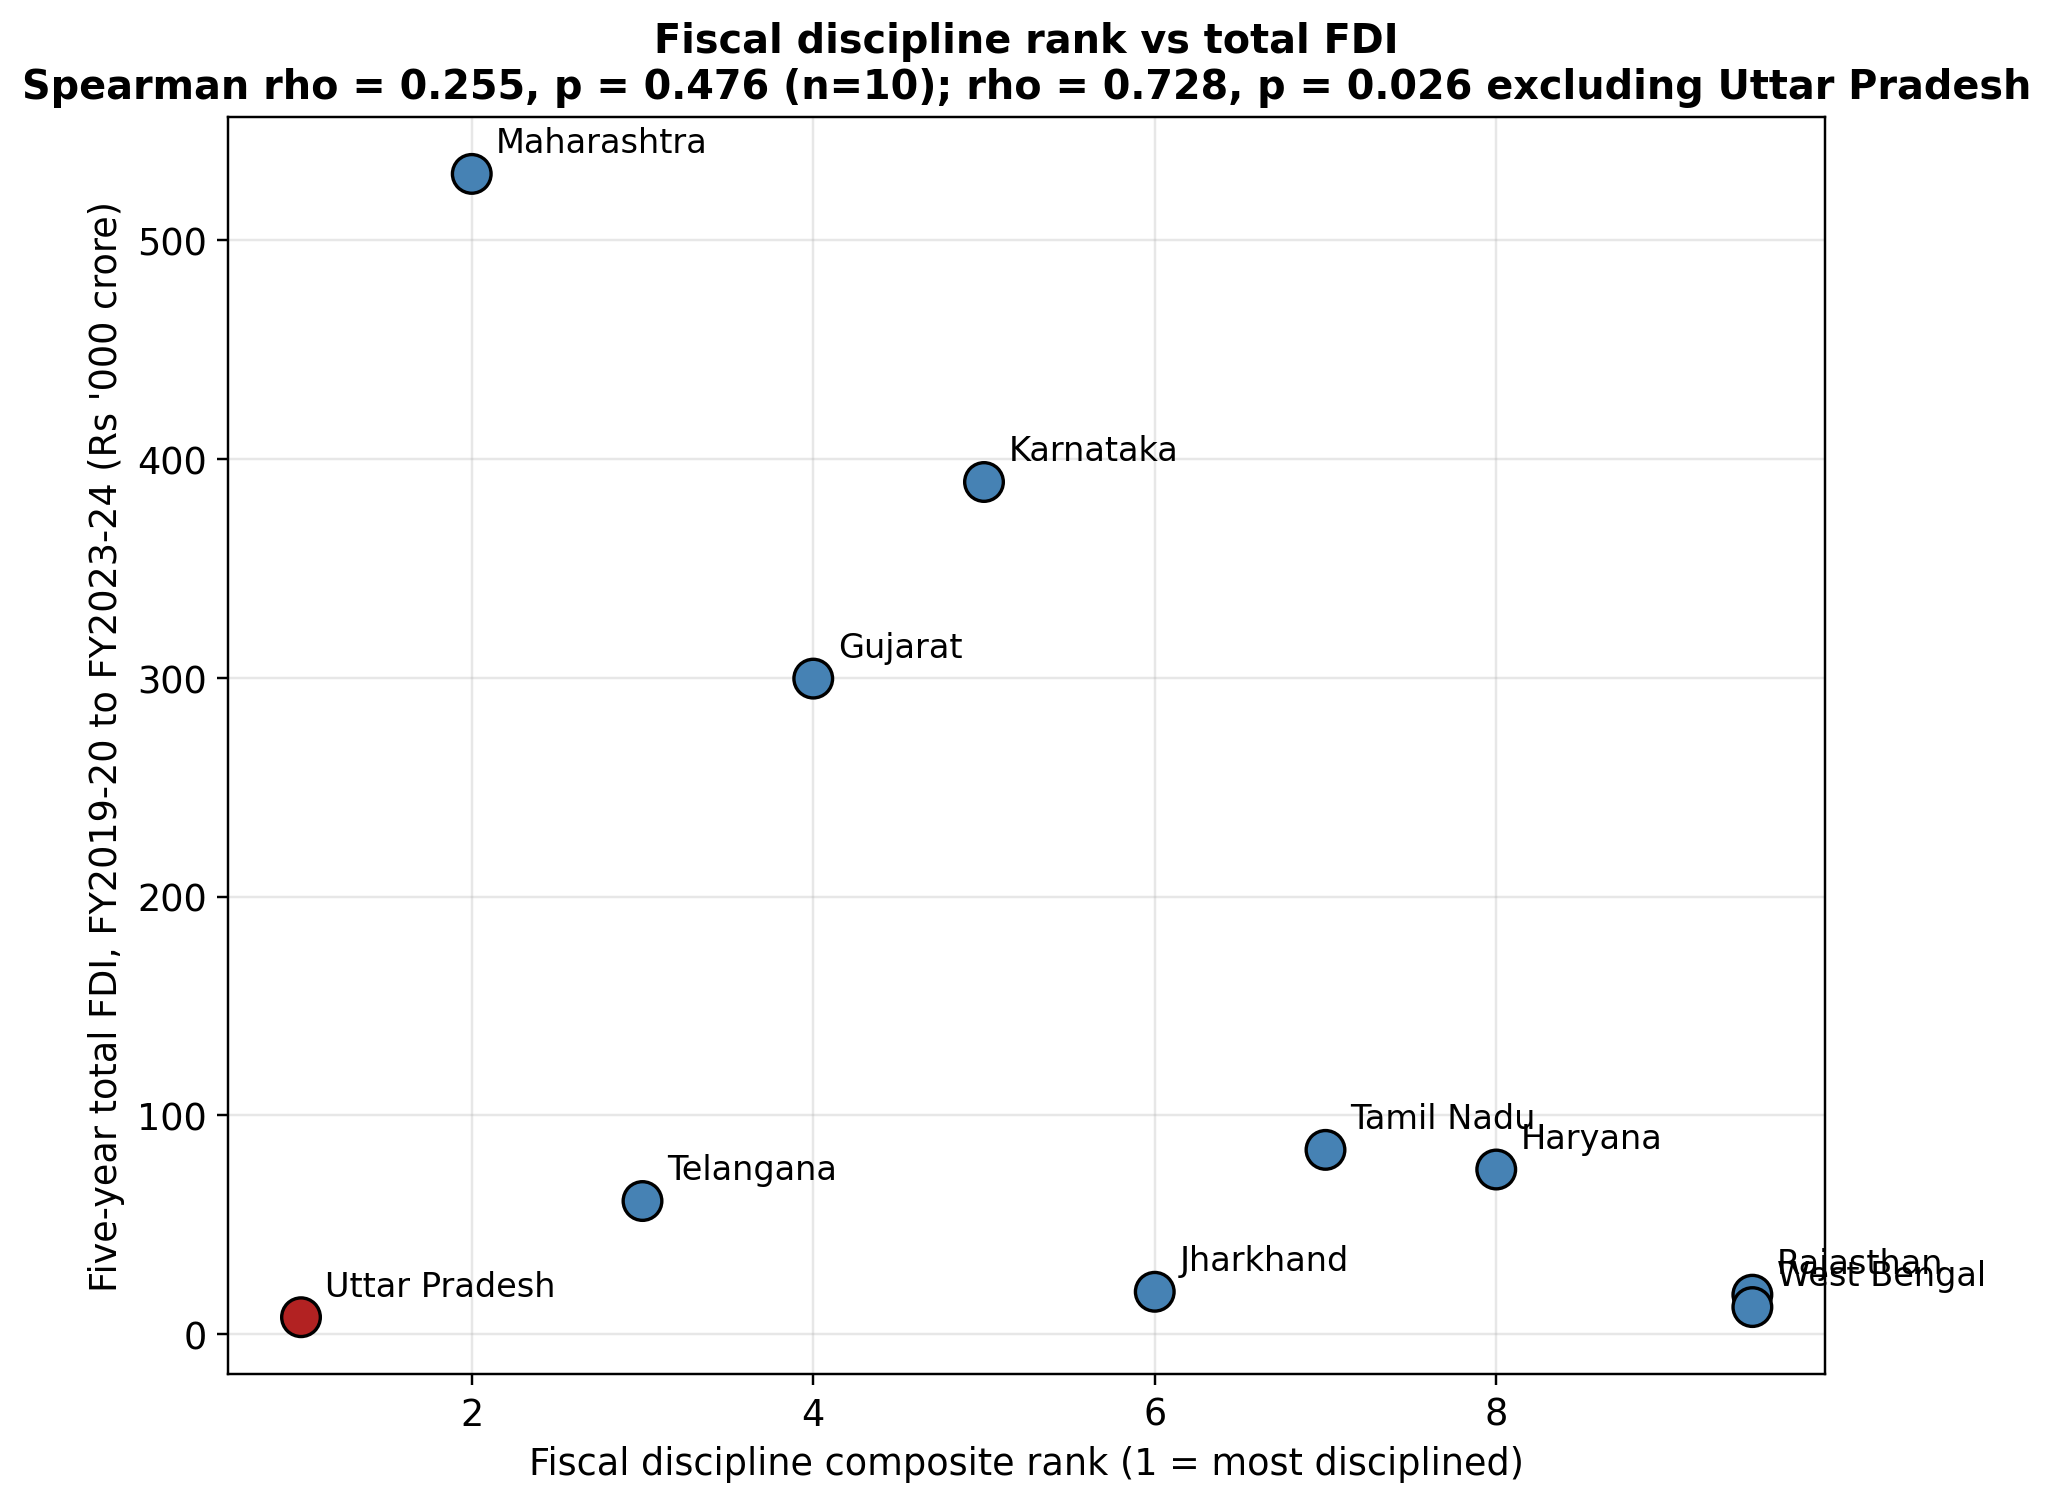
\includegraphics[width=0.78\textwidth]{figures/fig12.png}
\caption{Fiscal discipline composite rank plotted against five-year total FDI. Uttar Pradesh, whose FDI series is left-censored before FY 2021-22 and is therefore not a genuine low-FDI outcome, is marked in red; every other state is marked in blue. Excluding Uttar Pradesh, the downward slope implied by the remaining nine points is the significant Spearman correlation (rho = 0.728, p = 0.026) reported above.}
\label{fig:12}
\end{figure}

\begin{figure}[H]
\centering
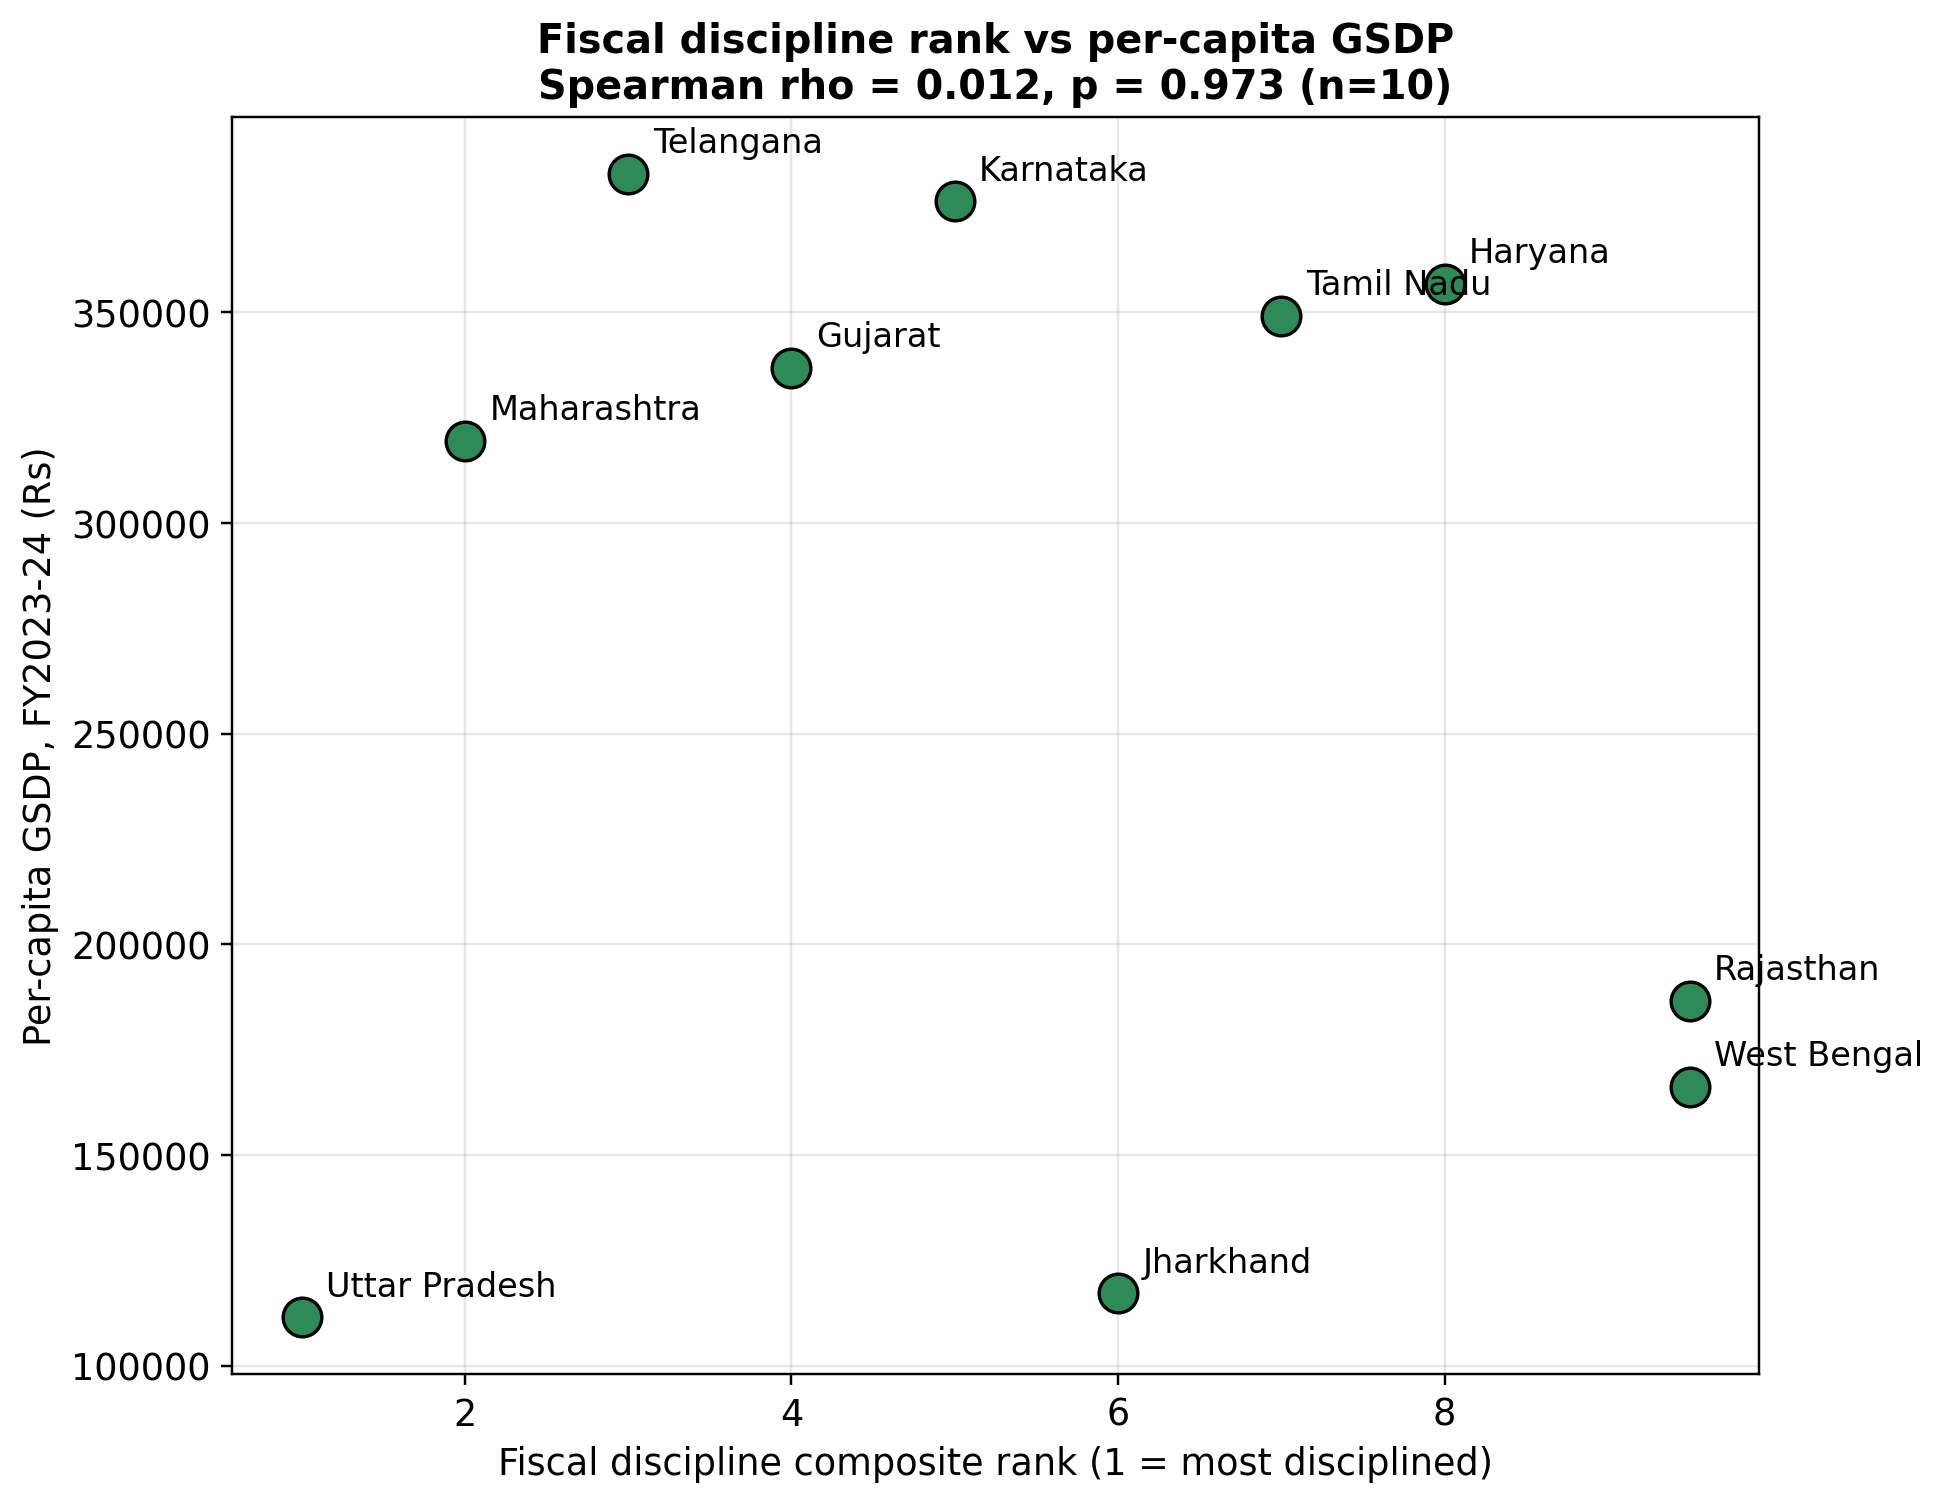
\includegraphics[width=0.74\textwidth]{figures/fig13.png}
\caption{Fiscal discipline composite rank plotted against FY 2023-24 per-capita GSDP. Unlike the FDI relationship in Figure 12 above, no clear pattern is visible, consistent with the statistically insignificant Spearman correlation (rho = 0.012, p = 0.973) reported above.}
\label{fig:13}
\end{figure}

\subsection{Panel regression: FDI (Model 1)}
The fixed-effects specification (n = 48, within R\textsuperscript{2} = 0.429, F(5,33) = 4.96, p = 0.0017) explains within-state variation in log FDI. Fiscal deficit (coefficient 0.566, p < 0.001), debt (0.353, p < 0.001) and the COVID dummy (-1.406, p < 0.001) are all significant; own tax revenue and capital expenditure are not. A poolability F-test strongly rejects the null of no entity effects (F(9,33) = 6.74, p < 0.001), confirming that state fixed effects are doing real work in this model and that pooling would be misspecified here.

The pooled specification with Census controls (n = 48, R\textsuperscript{2} = 0.643, between R\textsuperscript{2} = 0.874, F(7,40) = 10.29, p < 0.001) tells a different, and for the paper's central claim more important, story. Debt is significantly negative (coefficient -0.176, standard error 0.062, t = -2.84, p = 0.0071): a one-percentage-point-lower debt-to-GSDP ratio is associated with roughly 17.6 per cent higher FDI, holding the other regressors and the Census controls fixed. Literacy is also significant (0.101, p = 0.035); capital expenditure is negative and significant in this specification too (-0.366, p = 0.008), a result discussed in Section 7.2; fiscal deficit, own tax revenue, the COVID dummy, and urbanisation are not significant at conventional levels.

\begin{table}[H]
\centering
\caption{Model 1, log(FDI), fixed effects and pooled OLS. Each fiscal ratio is reported with its coefficient, standard error, t-statistic and p-value under each of the two specifications described in Section 5.1.}
\label{tab:19}
\footnotesize
\begin{adjustbox}{max width=\textwidth}
\begin{tabular}{@{}lrrrrrrrr@{}}
\toprule
& \multicolumn{4}{c}{FE + Driscoll--Kraay} & \multicolumn{4}{c}{Pooled OLS + controls} \\
\cmidrule(lr){2-5}\cmidrule(lr){6-9}
Variable & Coef. & SE & $t$ & $p$ & Coef. & SE & $t$ & $p$ \\
\midrule
Intercept & -2.6202 & 0.9754 & -2.6864 & 0.0112 & 3.6472 & 4.5738 & 0.7974 & 0.4299 \\
Fiscal deficit & 0.5660 & 0.0994 & 5.6926 & 0.0000 & 0.5665 & 0.5011 & 1.1304 & 0.2650 \\
Debt & 0.3533 & 0.0422 & 8.3728 & 0.0000 & -0.1760 & 0.0620 & -2.8388 & 0.0071 \\
Own tax revenue & 0.1068 & 0.2600 & 0.4108 & 0.6838 & 0.3251 & 0.2893 & 1.1237 & 0.2678 \\
Capital expenditure & -0.1730 & 0.3021 & -0.5725 & 0.5709 & -0.3659 & 0.1316 & -2.7796 & 0.0083 \\
COVID dummy & -1.4059 & 0.2373 & -5.9246 & 0.0000 & 0.5467 & 0.3829 & 1.4281 & 0.1610 \\
Literacy & --- & --- & --- & --- & 0.1006 & 0.0461 & 2.1804 & 0.0352 \\
Urbanisation & --- & --- & --- & --- & 0.0047 & 0.0410 & 0.1146 & 0.9093 \\
\bottomrule
\end{tabular}
\end{adjustbox}
\end{table}

The figure below plots the raw relationship the fixed-effects half of Table 19 summarises: average fiscal deficit against average log FDI for each state, with colour showing average debt.

\begin{figure}[H]
\centering
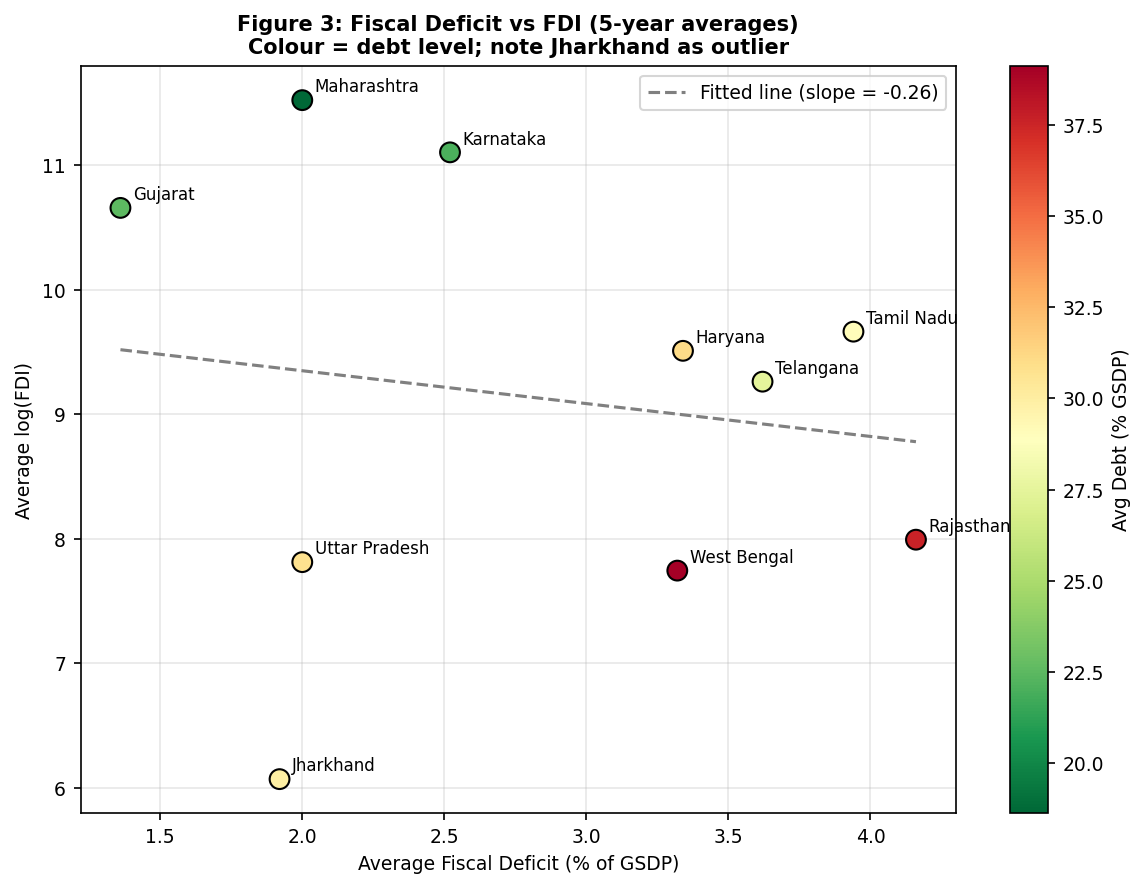
\includegraphics[width=0.74\textwidth]{figures/fig14.png}
\caption{Average fiscal deficit against average log FDI, five-year state means, colour-coded by average debt-to-GSDP (red = high debt, green = low debt). Jharkhand sits well off the fitted line, foreshadowing the case discussion in Section 7.3.}
\label{fig:14}
\end{figure}

The sign reversal on debt between the two specifications in Table 19 is the paper's central empirical fact and is addressed at length in Section 7.1; both coefficients are individually well estimated and neither is a coding artefact.

\subsection{Panel regression: GSDP growth (Model 2)}
For growth, the fixed-effects specification (n = 50, within R\textsuperscript{2} = 0.689, F(5,35) = 15.53, p < 0.001) shows fiscal deficit significantly negative (coefficient -2.172, p = 0.031) and debt significantly positive (1.097, p = 0.028); the COVID dummy is large and negative (-13.783, p < 0.001), consistent with the roughly 14-percentage-point growth collapse the panel records in FY 2020-21. Unlike Model 1, the poolability test for the growth equation does not reject pooling (F(9,35) = 0.82, p = 0.603), meaning the state fixed effects contribute comparatively little explanatory power once the fiscal variables and the COVID dummy are already in the equation.

\begin{table}[H]
\centering
\caption{Model 2, GSDP growth, fixed effects and pooled OLS, in the same layout as Table 19.}
\label{tab:20}
\footnotesize
\begin{adjustbox}{max width=\textwidth}
\begin{tabular}{@{}lrrrrrrrr@{}}
\toprule
& \multicolumn{4}{c}{FE + Driscoll--Kraay} & \multicolumn{4}{c}{Pooled OLS + controls} \\
\cmidrule(lr){2-5}\cmidrule(lr){6-9}
Variable & Coef. & SE & $t$ & $p$ & Coef. & SE & $t$ & $p$ \\
\midrule
Intercept & -37.9337 & 21.1480 & -1.7937 & 0.0815 & 5.3667 & 11.9457 & 0.4493 & 0.6556 \\
Fiscal deficit & -2.1719 & 0.9663 & -2.2477 & 0.0310 & -1.4353 & 1.4861 & -0.9658 & 0.3397 \\
Debt & 1.0967 & 0.4771 & 2.2984 & 0.0276 & 0.2579 & 0.2196 & 1.1744 & 0.2468 \\
Own tax revenue & 4.0830 & 2.4238 & 1.6845 & 0.1010 & 1.6267 & 0.8780 & 1.8528 & 0.0709 \\
Capital expenditure & -0.3560 & 1.2357 & -0.2881 & 0.7750 & -0.3226 & 0.9018 & -0.3578 & 0.7223 \\
COVID dummy & -13.7826 & 3.1731 & -4.3436 & 0.0001 & -12.6624 & 1.5744 & -8.0427 & 0.0000 \\
Literacy & --- & --- & --- & --- & -0.1720 & 0.1911 & -0.9004 & 0.3730 \\
Urbanisation & --- & --- & --- & --- & 0.1994 & 0.1355 & 1.4710 & 0.1487 \\
\bottomrule
\end{tabular}
\end{adjustbox}
\end{table}

The pooled growth specification (n = 50, R\textsuperscript{2} = 0.641, F(7,42) = 10.70, p < 0.001) is dominated by the COVID dummy (-12.662, p < 0.001); none of the four fiscal variables reach significance in this cross-state form, own tax revenue coming closest (1.627, p = 0.071). H2's support therefore comes specifically from the within-state, fixed-effects estimate, not from the cross-state comparison. That is the mirror image of the debt-FDI pattern in Model 1.

\subsection{Diagnostics and robustness}
Variance inflation factors for the four fiscal regressors range from 1.33 (capital expenditure) to 1.69 (debt), all comfortably below the conventional concern threshold of five, despite the mechanical link between deficits and debt (pairwise correlation 0.533; see the correlation matrix below). Multicollinearity is not a threat to either model's coefficient estimates.

\begin{table}[H]
\centering
\caption{Variance inflation factors, four fiscal regressors. A value near 1 means a regressor is close to uncorrelated with the others; values above 5 are the usual threshold for concern.}
\label{tab:21}
\footnotesize
\begin{adjustbox}{max width=\textwidth}
\begin{tabular}{@{}lr@{}}
\toprule
Variable & VIF \\
\midrule
const & 140.14 \\
Fiscal deficit & 1.52 \\
Debt & 1.69 \\
Own tax revenue & 1.51 \\
Capital expenditure & 1.33 \\
\bottomrule
\end{tabular}
\end{adjustbox}
\end{table}

\begin{table}[H]
\centering
\caption{Pairwise correlation matrix, fiscal regressors and outcome variables. Each cell is the Pearson correlation between the row and column variable across all state-year observations; the diagonal is 1 by construction.}
\label{tab:22}
\footnotesize
\begin{adjustbox}{max width=\textwidth}
\begin{tabular}{@{}lrrrrrr@{}}
\toprule
 & FD & Debt & OTR & CapEx & log FDI & Growth \\
\midrule
Fiscal deficit & 1.0 & 0.533 & -0.085 & -0.2 & -0.005 & -0.373 \\
Debt & 0.533 & 1.0 & -0.371 & -0.125 & -0.557 & -0.198 \\
Own tax revenue & -0.085 & -0.371 & 1.0 & 0.444 & 0.215 & 0.294 \\
Capital expenditure & -0.2 & -0.125 & 0.444 & 1.0 & -0.288 & 0.102 \\
log FDI & -0.005 & -0.557 & 0.215 & -0.288 & 1.0 & -0.113 \\
GSDP growth & -0.373 & -0.198 & 0.294 & 0.102 & -0.113 & 1.0 \\
\bottomrule
\end{tabular}
\end{adjustbox}
\end{table}

\begin{figure}[H]
\centering
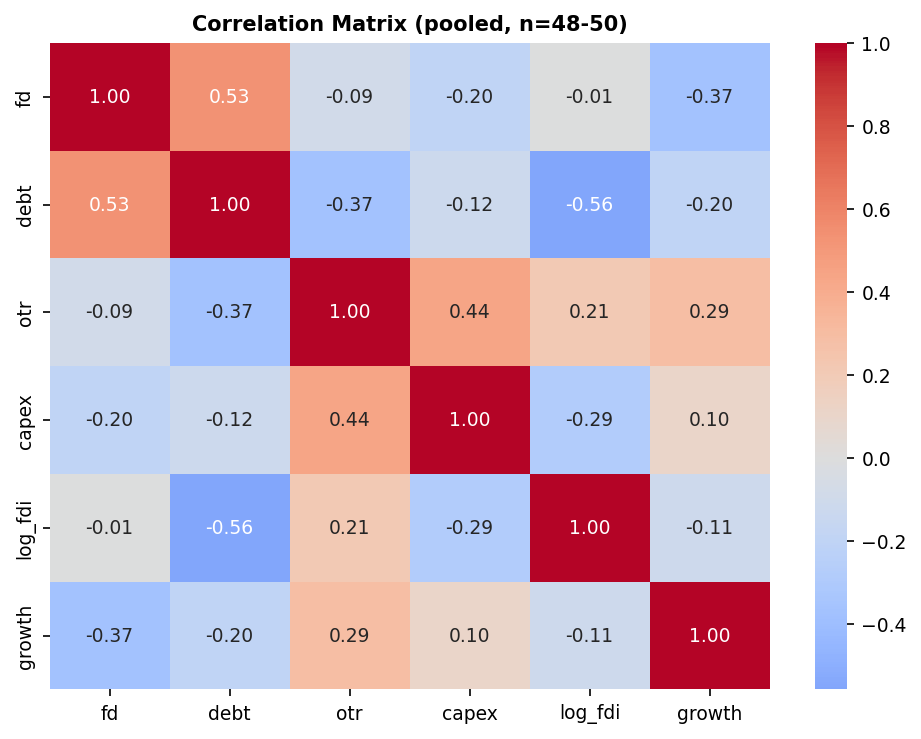
\includegraphics[width=0.71\textwidth]{figures/fig15.png}
\caption{Correlation heatmap of fiscal regressors and outcome variables, colour-coded from the same matrix as the table above (red = positive, blue = negative).}
\label{fig:15}
\end{figure}

The table below reports the within-state deficit and debt coefficients from Model 1 under three perturbations of the sample, to check whether the fixed-effects result is being driven by a single year or a single state. Dropping the COVID year (n = 39) leaves both coefficients stable in sign and significance (deficit 0.802, p = 0.017; debt 0.324, p = 0.002). Dropping Uttar Pradesh (n = 45) barely moves either estimate (deficit 0.532, p < 0.001; debt 0.366, p < 0.001), which matters because it shows the left-censoring in UP's FDI series is not driving the within-state result. Dropping Jharkhand (n = 43), by contrast, flips the deficit coefficient's sign and removes its significance entirely (-0.310, p = 0.141), while the debt coefficient survives, smaller but still significant (0.182, p = 0.015). Jharkhand alone is therefore responsible for a meaningful share of the within-state deficit-FDI pattern; Section 7.3 examines why.

\begin{table}[H]
\centering
\caption{Robustness of Model 1 within-state coefficients across four subsamples: the full baseline, then each perturbation dropping one problematic year or state in turn.}
\label{tab:23}
\footnotesize
\begin{adjustbox}{max width=\textwidth}
\begin{tabular}{@{}lrrrrrrrrr@{}}
\toprule
Specification & $n$ & FD coef & FD $p$ & Debt coef & Debt $p$ & OTR coef & OTR $p$ & CapEx coef & CapEx $p$ \\
\midrule
Baseline (all data) & 48 & 0.566 & 0.0 & 0.353 & 0.0 & 0.107 & 0.684 & -0.173 & 0.571 \\
Excl. COVID year (FY2020-21) & 39 & 0.802 & 0.017 & 0.324 & 0.002 & 0.535 & 0.26 & -0.207 & 0.48 \\
Excl. Jharkhand & 43 & -0.31 & 0.141 & 0.182 & 0.015 & 0.019 & 0.922 & 0.414 & 0.084 \\
Excl. Uttar Pradesh & 45 & 0.532 & 0.0 & 0.366 & 0.0 & 0.092 & 0.711 & -0.186 & 0.555 \\
\bottomrule
\end{tabular}
\end{adjustbox}
\end{table}

\subsection{Machine-learning validation}
The corrected specification (Section 5.2) restricts LASSO, Elastic Net and SHAP to the five time-varying fiscal regressors and re-estimates all three on the same 48 observations. LASSO, with its penalty strength chosen by leave-one-out cross-validation (alpha = 0.0011, a light penalty under which all five regressors survive), assigns debt-to-GSDP by far the largest standardised coefficient (-1.571), roughly twice the size of the next-largest, capital expenditure (-0.697); Elastic Net agrees closely (debt -1.478, capex -0.679).

\begin{table}[H]
\centering
\caption{LASSO and Elastic Net standardised coefficients, five fiscal predictors, ranked by the absolute size of the LASSO coefficient. A blank or zero coefficient would mean a variable was eliminated by the penalty; all five survive here.}
\label{tab:24}
\footnotesize
\begin{adjustbox}{max width=\textwidth}
\begin{tabular}{@{}lrlrl@{}}
\toprule
Variable & LASSO coef & LASSO sel. & E-Net coef & E-Net sel. \\
\midrule
Debt-to-GSDP & -1.5712 & YES & -1.4782 & YES \\
Fiscal Deficit & 0.728 & YES & 0.6523 & YES \\
Capital Expenditure & -0.697 & YES & -0.6788 & YES \\
COVID year & 0.22 & YES & 0.2252 & YES \\
Own Tax Revenue & 0.1572 & YES & 0.1736 & YES \\
\bottomrule
\end{tabular}
\end{adjustbox}
\end{table}

\begin{figure}[H]
\centering
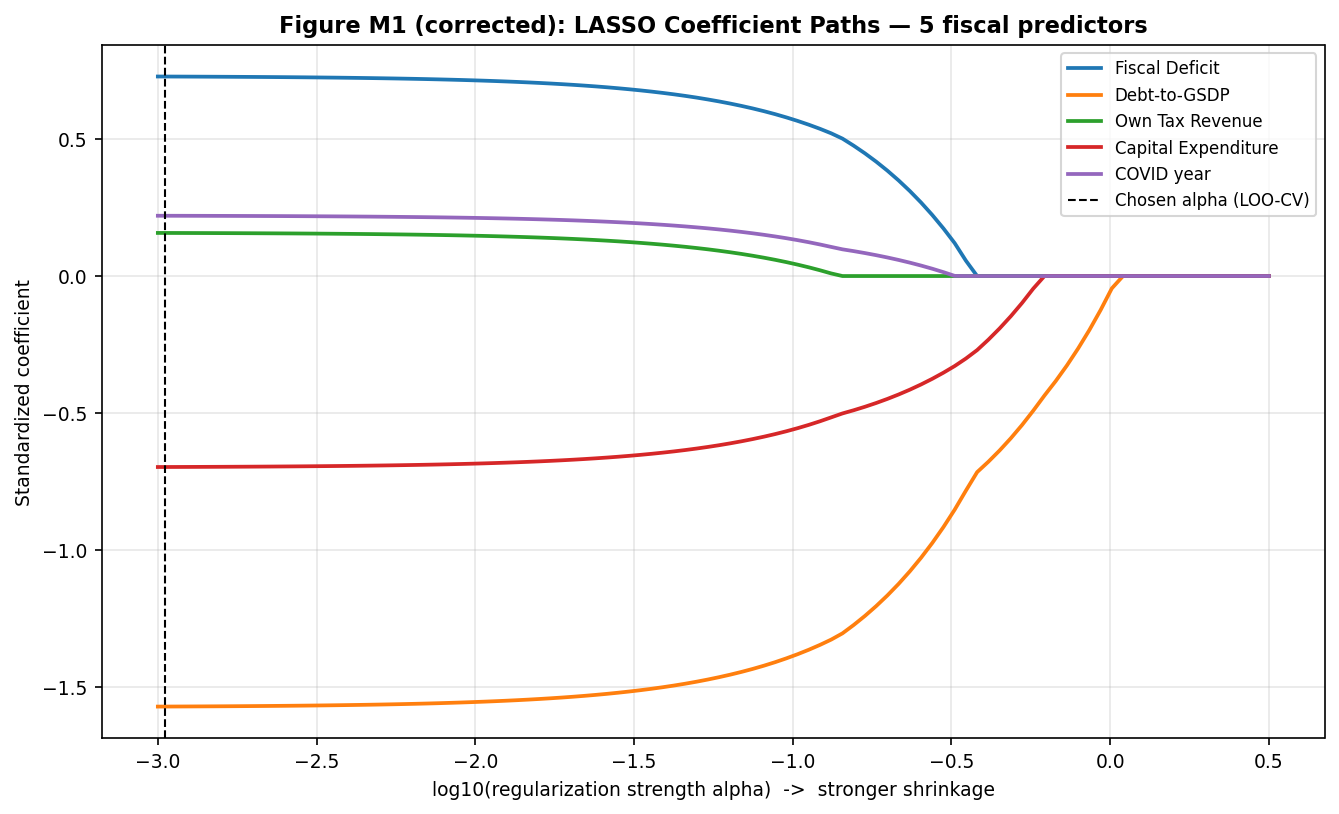
\includegraphics[width=0.94\textwidth]{figures/fig16.png}
\caption{LASSO coefficient paths across the regularisation path, five fiscal predictors. Each line traces one variable's coefficient as the penalty strength increases (moving right); the vertical dashed line marks the cross-validated penalty actually used in Table 24.}
\label{fig:16}
\end{figure}

\begin{figure}[H]
\centering
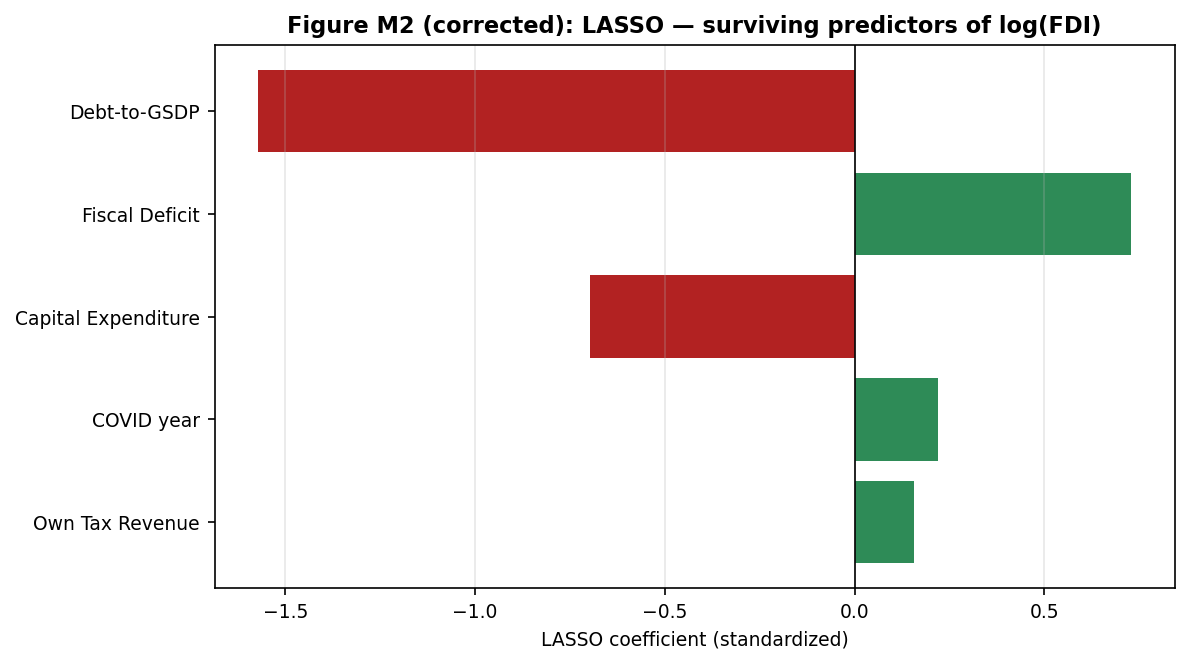
\includegraphics[width=1.00\textwidth]{figures/fig17.png}
\caption{LASSO surviving coefficients at the cross-validated regularisation strength, five fiscal predictors, plotted as a bar for each variable's final coefficient.}
\label{fig:17}
\end{figure}

The leave-one-state-out stability check refits LASSO ten times, each time leaving one state's five observations out entirely, to confirm that debt's dominance is not an artefact of any single state. Debt is selected in all ten refits, alongside capital expenditure and own tax revenue; only fiscal deficit is dropped in one of the ten refits.

\begin{table}[H]
\centering
\caption{LASSO selection frequency across ten leave-one-state-out refits: the number of times, out of ten, each variable survived the LASSO penalty when one state was excluded from the estimation sample.}
\label{tab:25}
\footnotesize
\begin{adjustbox}{max width=\textwidth}
\begin{tabular}{@{}lr@{}}
\toprule
Variable & Times\_selected\_out\_of\_10\_state-leave-out\_refits \\
\midrule
Debt-to-GSDP & 10 \\
Capital Expenditure & 10 \\
Own Tax Revenue & 10 \\
COVID year & 10 \\
Fiscal Deficit & 9 \\
\bottomrule
\end{tabular}
\end{adjustbox}
\end{table}

SHAP values from the corrected random forest (out-of-bag R\textsuperscript{2} = 0.402) rank debt-to-GSDP first among the five predictors by a wide margin: mean \textbar{}SHAP\textbar{} = 1.029, against 0.219 for fiscal deficit, 0.208 for own tax revenue, 0.136 for capital expenditure, and an effectively negligible 0.007 for the COVID dummy.

\begin{table}[H]
\centering
\caption{SHAP importance, five fiscal predictors, random forest. Mean \textbar{}SHAP\textbar{} is the average, across all 48 observations, of the absolute contribution that variable made to the model's prediction for that observation; a higher value means the variable moves the predicted FDI further, in either direction.}
\label{tab:26}
\footnotesize
\begin{adjustbox}{max width=\textwidth}
\begin{tabular}{@{}lr@{}}
\toprule
Variable & Mean $|$SHAP$|$ \\
\midrule
Debt-to-GSDP & 1.0287 \\
Fiscal Deficit & 0.2185 \\
Own Tax Revenue & 0.2081 \\
Capital Expenditure & 0.136 \\
COVID year & 0.0068 \\
\bottomrule
\end{tabular}
\end{adjustbox}
\end{table}

\begin{figure}[H]
\centering
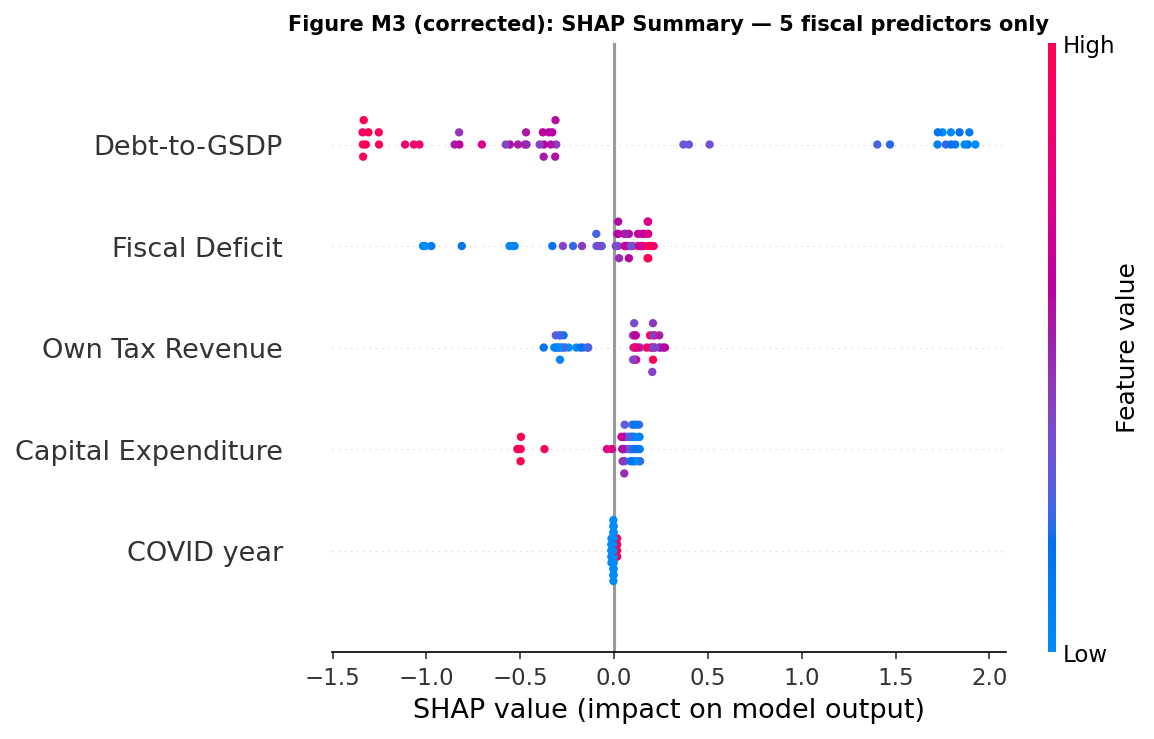
\includegraphics[width=0.89\textwidth]{figures/fig18.png}
\caption{SHAP summary plot, five fiscal predictors. Each dot is a single state-year. Its horizontal position gives that observation's SHAP value, the pull it exerted on predicted log FDI, and its colour gives the observation's value on the variable itself (red high, blue low). In the debt row the red dots sit to the left, on the negative side: high debt pushes predicted FDI down.}
\label{fig:18}
\end{figure}

\begin{figure}[H]
\centering
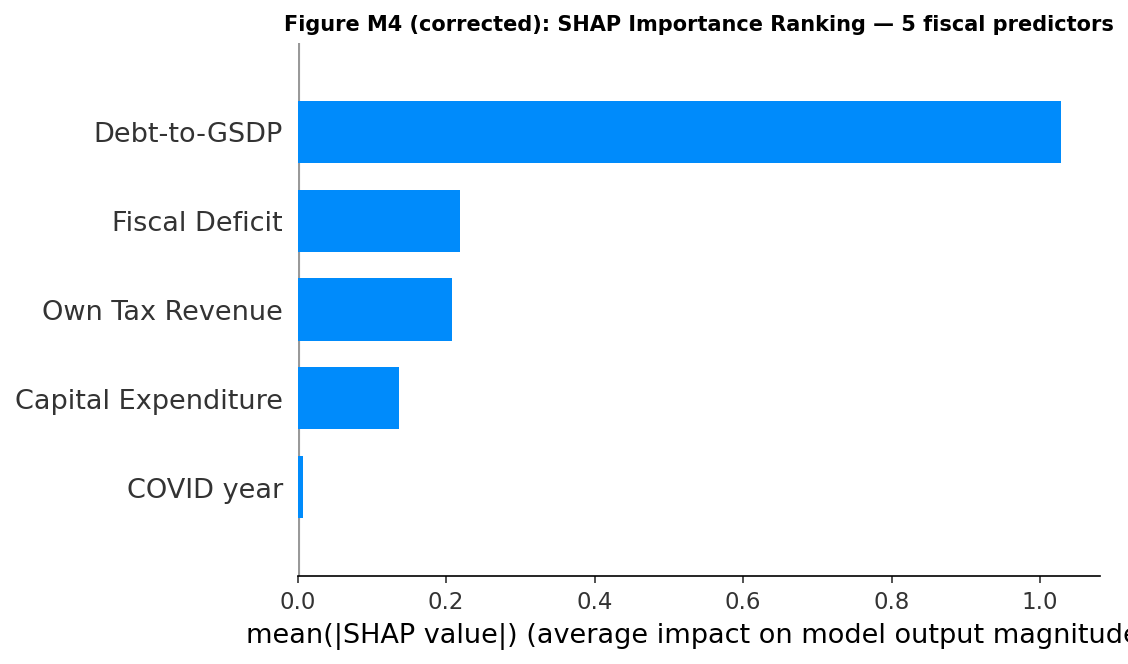
\includegraphics[width=0.97\textwidth]{figures/fig19.png}
\caption{SHAP importance by mean absolute SHAP value, five fiscal predictors. The same ranking as Table 26, drawn as bars.}
\label{fig:19}
\end{figure}

\begin{figure}[H]
\centering
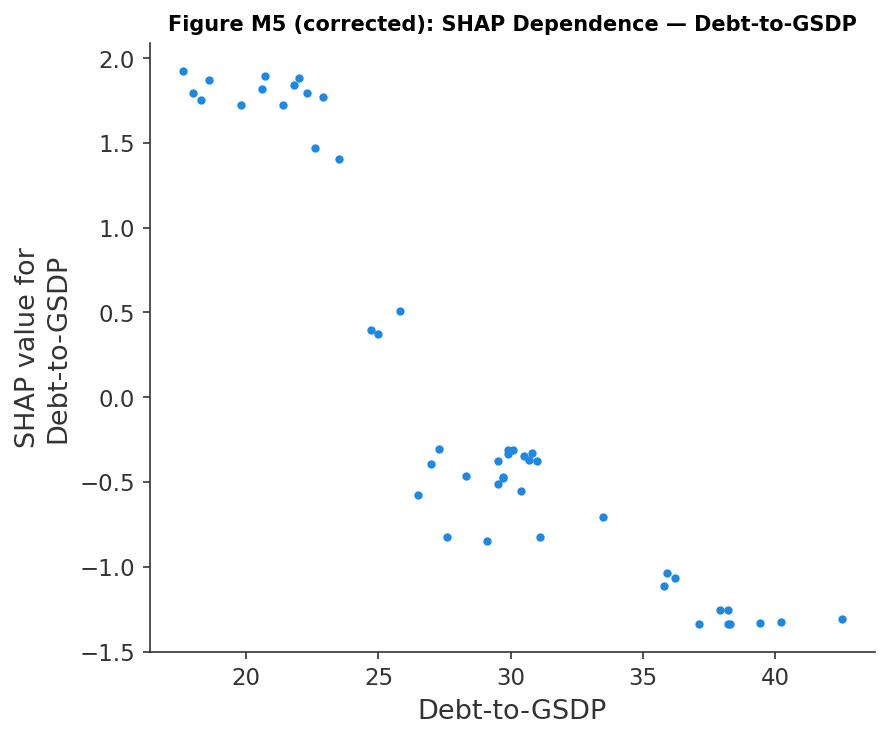
\includegraphics[width=0.69\textwidth]{figures/fig20.png}
\caption{SHAP dependence plot for debt-to-GSDP. Horizontal position is the state-year's debt ratio and vertical position is that observation's SHAP value, so the plot traces the effect on predicted log FDI across the range of debt the panel actually covers.}
\label{fig:20}
\end{figure}

Out-of-sample R-squared under leave-one-out cross-validation is modest across the board, which is what forty-eight observations should produce: 0.440 for OLS, 0.416 for LASSO, 0.395 for the random forest. None of the three is a claim to predictive power. The exercise validates an in-sample ranking; it does not forecast. That the three numbers sit so close together carries its own information, though. The extra flexibility of the forest buys no out-of-sample accuracy here, which is what one would expect if the underlying relationship is close to linear once debt is in the model.

\begin{table}[H]
\centering
\caption{Leave-one-out out-of-sample R-squared, five fiscal predictors: each model is refit 48 times, once per observation left out, and R-squared is computed on the held-out predictions.}
\label{tab:27}
\footnotesize
\begin{adjustbox}{max width=\textwidth}
\begin{tabular}{@{}lr@{}}
\toprule
Model & LOO-CV out-of-sample $R^2$ \\
\midrule
OLS (5 predictors) & 0.44 \\
LASSO (selected subset) & 0.416 \\
Random Forest & 0.395 \\
\bottomrule
\end{tabular}
\end{adjustbox}
\end{table}

Three methodologically independent approaches therefore converge on debt-to-GSDP as the dominant fiscal predictor of cross-state FDI: a pooled panel regression, a regularised linear selector, and a non-linear tree-based explainer. The sign is negative in all three. Together with the Spearman correlation of Section 6.2, this convergence is the strongest evidence the paper offers for H1 in its cross-state form, precisely because it does not rest on any single model's distributional assumptions, nor on treating one p = 0.007 result as sufficient in a panel this short.

\FloatBarrier
\section{Discussion}
\subsection{Why debt is negative between states and positive within them}
The central puzzle in Section 6.3 is that debt enters Model 1 negative and significant in the pooled cross-state specification, and positive and significant in the within-state fixed-effects specification. Both estimates are correct. They answer different questions. The pooled coefficient asks whether a state that persistently carries less debt than its peers attracts more FDI than they do. It does, and the magnitude, roughly 18 per cent more FDI per percentage point of lower debt-to-GSDP, lines up with the discipline ranking of Section 4.7. The two lowest-debt states in the panel, Gujarat and Maharashtra, rank first or second overall in almost every year; the highest-debt state, West Bengal, ranks last in all five. It lines up too with the Spearman correlation of Section 6.2, which turns significant (rho = 0.728, p = 0.026) once the one state whose FDI series is an accounting artefact rather than a genuine low outcome is set aside.

The fixed-effects coefficient asks something narrower: within a given state, in the years when its own debt ratio rose above its own average, did its own FDI rise too? Again yes, but for a reason that has nothing to do with fiscal virtue. The panel has five years. One of them, FY 2020-21, is a pandemic year in which every state's deficit and debt jumped at the same moment as a national FDI collapse. National FDI then recovered through FY 2021-22 and FY 2022-23, and in several states that recovery coincided with debt still elevated by pandemic-era borrowing. Gujarat's FDI surge in FY 2020-21 and Karnataka's in FY 2021-22 both occurred while debt sat above pre-pandemic levels nationally. With only five time periods, one common shock of that size can dominate the within-state covariance between any two variables that moved sharply around it, and debt and the post-pandemic FDI recovery are exactly such a pair.

The practical reading we draw is that fiscal discipline works as a structural, between-state signal that investors use to compare states with one another. It is not a lever a single state can pull in one budget year to move its own inflows. A finance department that cuts its deficit by half a percentage point this year should not expect that action alone to shift next year's FDI number. A state that has held debt below 25 per cent of GSDP for five consecutive years is operating in a different competitive tier from one that has not, and the market appears to price that difference.

\subsection{Capital expenditure's negative sign}
Capital expenditure enters the pooled FDI specification negative and significant (-0.366, p = 0.008). That is the wrong sign for the crowding-in channel of Section 2. Two properties of the measure account for it without forcing the channel to be abandoned outright. The first is construction. Capex here is derived as gross fiscal deficit minus revenue deficit (Section 4.2), so it carries net lending with it, and a state lending heavily to its public-sector undertakings records high derived capex while building nothing an investor would notice. The second is its correlation with debt, which runs the wrong way for the crowding-in story. Several of the higher-debt, lower-FDI states in this panel also post higher derived capex, because borrowed money spent on capital account is still capex even when the borrowing itself is the more informative signal. The coefficient should therefore be read alongside debt rather than on its own. Capex financed from a low debt base and the same nominal capex financed from a high one are different signals to an investor, and one linear coefficient cannot separate them. Interacting capex with its financing source is the obvious extension once a longer panel exists.

\subsection{The Jharkhand and Uttar Pradesh cases}
Jharkhand is the panel's clearest case of discipline failing to convert into investment. Its composite rank is 6 of 10 (5.8 on the year-wise average, Section 4.7), squarely mid-table, yet its FDI path is among the sharpest in the sample: a spike in FY 2019-20, then near-total collapse from FY 2020-21 onward. Section 6.5 shows what this does to the estimates. Remove Jharkhand and the within-state deficit coefficient goes from significantly positive to indistinguishable from zero. Its own trajectory, a widening deficit alongside disappearing FDI, is the mirror image of what Gujarat and Karnataka record, and it is carrying a real share of the within-state result. We keep it rather than trim it. Discipline looks like something investors screen on, and Jharkhand shows that screening in is not the same as being chosen. Political transition, the investment cycle particular to mining, and an infrastructure deficit relative to the western and southern states in the sample are all plausible candidates for the residual, and none of them is modelled here.

Uttar Pradesh is a different kind of problem. DPIIT's series for the state starts in FY 2021-22, so its first two panel years are missing rather than genuinely zero (Section 4.5). Since Uttar Pradesh ranks at or near the top on discipline throughout (composite rank 1 of 10; 2.2 on the year-wise average, tied for best), one might reasonably suspect the censoring of inflating the debt-FDI relationship by association. Section 6.5 tests that directly and rules it out. Dropping Uttar Pradesh moves the deficit and debt coefficients by hundredths and leaves both significant. The censoring does bite elsewhere, on the Spearman correlation of Section 6.2, which is insignificant with the state included and significant without it. Both diagnostics behave exactly as they should. The regression uses year-by-year variation and is unmoved by the two missing cells; the rank correlation compresses each state to one point, and in a sample of ten a single mismatched point of that size is enough to flatten it.

\subsection{What the agglomeration rival hypothesis survives}
Section 3 set agglomeration against the fiscal channels: FDI follows existing clusters, and the host government's balance sheet is beside the point. The evidence assembled here does not settle that argument. It locates fiscal discipline inside it. Recall the uncorrected SHAP run of Section 5.2, which included Census urbanisation and ranked it far above every fiscal variable (mean \textbar{}SHAP\textbar{} = 1.30 against 0.25 for debt). Part of that gap was the state-identity leakage diagnosed and corrected in Section 6.6. Part of it was probably real, since urbanisation proxies quite well for the clustering and market-size effects agglomeration describes. Once the machine-learning stage is confined to variables that move within a state over time, the same set the fixed-effects model uses, debt dominates them. The honest synthesis is that the two explanations operate at different levels rather than competing directly. Fixed structural advantages, geography and an existing industrial base, plausibly determine which states are in the top ten at all. Fiscal discipline then sorts investment within that already-favoured group. That reading fits the between-state result of Section 7.1, and it rules out the stronger claim that fiscal policy is irrelevant once agglomeration has been accounted for.

\FloatBarrier
\section{Conclusion, Policy Implications and Limitations}
Sub-national fiscal discipline is associated with more FDI in India, but the relationship holds between states rather than within them over the five years examined here. States that have kept debt low relative to GSDP, Gujarat and Maharashtra foremost among the ten studied, attract significantly more FDI than states that have not. Five methods replicate that finding: a pooled panel regression, a Spearman rank correlation, LASSO, Elastic Net, and SHAP-based random forest importance. They share no common statistical assumption beyond the same forty-eight to fifty observations. Fiscal deficit is separately associated with lower GSDP growth within states over time, replicating Trivedi and Rajmal (2011) and Panda and Sahay (2022) on a newer, audited, post-pandemic panel.

The distinction between the two dimensions is the finding with the most practical content, and it is worth stating plainly before any policy reading is drawn from it. Debt predicts FDI when states are compared with one another. It does not predict FDI when a single state is compared with its own past over these five years. On the evidence assembled here, fiscal discipline is a standing characteristic that investors appear to price, not an annual instrument that moves investment in the year it is exercised. Whether the within-state estimate would look different over a window not dominated by a pandemic is an open question, and Section 7.1 gives the reason to expect that it would.

Three implications follow for state finance departments. The first concerns time horizon. If the investment-relevant signal is a state's persistent position relative to its peers, then consolidation is a multi-year credibility investment rather than a single-budget lever, and it should be evaluated on that basis. A department that reduces its deficit by half a percentage point in one year and expects a visible FDI response the next is applying the wrong test to its own policy, and is likely to abandon a correct policy for want of a result. The second concerns which indicator to anchor on. Of the four examined here, debt is the one every method selects, and it is also the one an outside observer can verify most easily from published accounts. Deficit matters for growth, and the growth result in Section 6.4 is not weak, but the investment-facing signal in this sample is the stock rather than the flow. The third concerns expenditure composition. The negative pooled coefficient on capital expenditure discussed in Section 7.2 should not be read as an argument against capital spending. It is an argument about how capital spending is financed, and about a derived measure that carries net lending inside it. Capex funded from a low debt base and the same nominal capex funded by fresh borrowing are different propositions to an investor, and a state that treats them as equivalent is misunderstanding what its own accounts communicate.

For the Finance Commission, for NITI Aayog, and for the investment-promotion bodies that cite their rankings, the implication is narrower but sharper. A fiscal discipline ranking becomes informative once it is validated against an outcome, as it is here, and remains merely arithmetic when it is published as an end in itself. That is not a call to abolish such indices. It is a call to report, alongside the ranking, the correlation between the ranking and something observable: investment received, growth recorded, borrowing costs paid. Doing so would make the weighting scheme falsifiable, which at present it is not. Our own composite ranking is offered in exactly that spirit. It is reported in Section 4.7, its construction is given in full with a worked example so that it can be recomputed or disputed, and it is then tested against FDI and per-capita GSDP in Section 6.2, where it passes the first test and fails the second. Reporting the failure is part of the point.

Jharkhand is a caution against reading any ranking mechanically. It sits mid-table on discipline and near the bottom on realised investment, and its trajectory does real work in the within-state estimates. Discipline appears necessary; Jharkhand demonstrates that it is not sufficient. A state government that improves its fiscal position without addressing the sector-specific and region-specific frictions an investor also weighs, whether infrastructure gaps, land and clearance processes, or the particular investment cycle of a dominant industry, should not expect FDI to follow automatically. The reverse caution applies to Uttar Pradesh, whose apparent weakness on the investment side is an artefact of when DPIIT began reporting its series rather than a statement about the state.

Four limitations bound these conclusions, and the first is simply arithmetic. The panel is short: fifty state-year cells, forty-eight of them with a usable FDI observation. That is why the paper leans on convergent machine-learning and rank-correlation evidence instead of the regression p-values alone, and why instrument-heavy dynamic panel GMM was excluded by design at this N and T (Roodman, 2009). A short panel also means that any single influential year or state can move a coefficient materially, which is precisely what Section 6.5 documents for Jharkhand.

Second, FDI recording is itself imperfect. DPIIT's state-wise series begins in October 2019, which makes FY 2019-20 a six-month flow rather than a full year, and it leaves Uttar Pradesh censored until FY 2021-22. Section 6.5 addresses both but cannot remove either. A further measurement caveat applies to the FDI variable generally: equity inflows are recorded against the state of the recipient company's registered office, which need not be the state where the capital is ultimately deployed, and this will tend to overstate flows to states hosting corporate headquarters.

Third, the debt measure is the official on-budget figure taken from CAG-audited finance accounts. It excludes off-budget borrowings and guarantees, which for Telangana alone have been estimated at roughly 14 to 15 per cent of GSDP, large enough to change any assessment of true fiscal risk. Since the paper's central result is about debt specifically, this is the limitation most likely to matter for the size of the estimated effect, though its direction is not obvious in advance: if off-budget exposure is concentrated among states already ranked as high-debt, including it would widen the spread and strengthen the result, while if it is concentrated among low-recorded-debt states it would compress it.

Fourth, association is all that a five-year panel of ten states can support. Reverse causality, in which anticipated investment changes a state's fiscal behaviour rather than the other way round, cannot be ruled out by this design. Nor can the sample speak to states outside the top ten. The ten states studied here are the ten that already receive almost all of India's FDI, so the result should be read as describing how investment is sorted among states that are already candidates for it, not as a claim that a low-FDI state can enter that group by consolidating its balance sheet alone. Section 7.4 argues that agglomeration and fiscal discipline plausibly operate at those two different levels, and nothing in this design can separate them fully.

It is worth stating what would change this conclusion, since a finding that cannot be overturned is not much of a finding. Three observations would do it. A longer panel in which the between-state debt coefficient loses significance once further post-pandemic years are added would indicate that the present result is a feature of the COVID window rather than a standing relationship. A debt measure extended to include off-budget guarantees that reversed the ranking of the high-debt and low-debt groups would undercut the interpretation even if the coefficient survived. And a specification in which a direct agglomeration measure, rather than the Census proxy used here, absorbed the debt effect entirely would support the rival hypothesis of Section 3 over the reading offered in Section 7.4.

Three extensions follow from those limits. A longer panel, once further post-pandemic years have been audited, would show whether the within-state debt coefficient moves toward the between-state sign as FY 2020-21 loses weight in the estimation window; Section 7.1 predicts that it should. Adding off-budget guarantees to the debt measure, and interacting capital expenditure with its financing source, are the two specification changes that Section 7.2 and the limitations above point to most directly. Beyond this sample, the natural test of external validity is to extend the panel below the top ten, where the variation in both fiscal position and investment is wider and the agglomeration floor is lower, and to ask whether the same convergence across methods survives outside the group of states that were always going to receive the capital.

\FloatBarrier

\FloatBarrier
\section*{References}
\small
\hangindent=0.5in\hangafter=1
Arellano, M., \& Bond, S. (1991). Some tests of specification for panel data: Monte Carlo evidence and an application to employment equations. Review of Economic Studies, 58(2), 277-297. \url{https://doi.org/10.2307/2297968}

\hangindent=0.5in\hangafter=1
Athey, S., \& Imbens, G. W. (2019). Machine learning methods that economists should know about. Annual Review of Economics, 11, 685-725. \url{https://doi.org/10.1146/annurev-economics-080217-053433}

\hangindent=0.5in\hangafter=1
Baltagi, B. H. (2021). Econometric analysis of panel data (6th ed.). Springer. \url{https://doi.org/10.1007/978-3-030-53953-5}

\hangindent=0.5in\hangafter=1
Barro, R. J. (1990). Government spending in a simple model of endogenous growth. Journal of Political Economy, 98(5, Pt. 2), S103-S125. \url{https://doi.org/10.1086/261726}

\hangindent=0.5in\hangafter=1
Blonigen, B. A. (2005). A review of the empirical literature on FDI determinants. Atlantic Economic Journal, 33(4), 383-403. \url{https://doi.org/10.1007/s11293-005-2868-9}

\hangindent=0.5in\hangafter=1
Borensztein, E., De Gregorio, J., \& Lee, J.-W. (1998). How does foreign direct investment affect economic growth? Journal of International Economics, 45(1), 115-135. \url{https://doi.org/10.1016/S0022-1996(97)00033-0}

\hangindent=0.5in\hangafter=1
Breiman, L. (2001). Random forests. Machine Learning, 45(1), 5-32. \url{https://doi.org/10.1023/A:1010933404324}

\hangindent=0.5in\hangafter=1
Department for Promotion of Industry and Internal Trade (DPIIT). (2024). State-wise FDI equity inflows (from October 2019). Ministry of Commerce and Industry, Government of India. \url{https://dpiit.gov.in}

\hangindent=0.5in\hangafter=1
Driscoll, J. C., \& Kraay, A. C. (1998). Consistent covariance matrix estimation with spatially dependent panel data. Review of Economics and Statistics, 80(4), 549-560. \url{https://doi.org/10.1162/003465398557825}

\hangindent=0.5in\hangafter=1
Drukker, D. M. (2003). Testing for serial correlation in linear panel-data models. Stata Journal, 3(2), 168-177. \url{https://doi.org/10.1177/1536867X0300300206}

\hangindent=0.5in\hangafter=1
Dunning, J. H. (1993). Multinational enterprises and the global economy. Addison-Wesley. \url{https://archive.org/details/multinationalent0000dunn}

\hangindent=0.5in\hangafter=1
Feld, L. P., K\"ohler, E. A., Palhuca, L., \& Schaltegger, C. A. (2024). Fiscal federalism and foreign direct investment: An empirical analysis. The World Economy, 47(6), 2287-2331. \url{https://doi.org/10.1111/twec.13547}

\hangindent=0.5in\hangafter=1
Fischer, S. (1993). The role of macroeconomic factors in growth. Journal of Monetary Economics, 32(3), 485-512. \url{https://doi.org/10.1016/0304-3932(93)90027-D}

\hangindent=0.5in\hangafter=1
Government of India. (2025). Report of the Sixteenth Finance Commission, Volume II: Annexures. Ministry of Finance. \url{https://indiabudget.gov.in/doc/16fcvol2.pdf}

\hangindent=0.5in\hangafter=1
Hastie, T., Tibshirani, R., \& Friedman, J. (2009). The elements of statistical learning: Data mining, inference, and prediction (2nd ed.). Springer. \url{https://doi.org/10.1007/978-0-387-84858-7}

\hangindent=0.5in\hangafter=1
Hausman, J. A. (1978). Specification tests in econometrics. Econometrica, 46(6), 1251-1271. \url{https://doi.org/10.2307/1913827}

\hangindent=0.5in\hangafter=1
International Monetary Fund. (2020). World economic outlook, April 2020: The great lockdown. IMF. \url{https://www.imf.org/en/publications/weo/issues/2020/04/14/weo-april-2020}

\hangindent=0.5in\hangafter=1
Lundberg, S. M., \& Lee, S.-I. (2017). A unified approach to interpreting model predictions. Advances in Neural Information Processing Systems, 30, 4765-4774. \url{https://arxiv.org/abs/1705.07874}

\hangindent=0.5in\hangafter=1
Mahatekar, D. D. (2025). State-wise foreign direct investment (FDI) flows and economic impacts in India: A comparative study (2019-2024). JETIR, 12(10). \url{https://www.jetir.org/papers/JETIR2510525.pdf}

\hangindent=0.5in\hangafter=1
Ministry of Statistics and Programme Implementation (MoSPI). (2024). State-wise Gross State Domestic Product, 2011-12 series. Government of India. \url{https://mospi.gov.in}

\hangindent=0.5in\hangafter=1
Misra, S., Gupta, K., \& Trivedi, P. (2021). Sub-national government debt sustainability in India: An empirical analysis. Macroeconomics and Finance in Emerging Market Economies, 16(1), 57-79. \url{https://doi.org/10.1080/17520843.2021.1948171}

\hangindent=0.5in\hangafter=1
Mullainathan, S., \& Spiess, J. (2017). Machine learning: An applied econometric approach. Journal of Economic Perspectives, 31(2), 87-106. \url{https://doi.org/10.1257/jep.31.2.87}

\hangindent=0.5in\hangafter=1
National Institute of Public Finance and Policy (NIPFP). (2024). How much debt is optimal for the major Indian states? Economic growth vs. debt sustainability (Working Paper No. 411). \url{https://nipfp.org.in/media/documents/WP_411_2024.pdf}

\hangindent=0.5in\hangafter=1
NITI Aayog. (2025). Fiscal Health Index 2025. Government of India. \url{https://niti.gov.in}

\hangindent=0.5in\hangafter=1
NITI Aayog. (2026). Fiscal Health Index 2026. Government of India. \url{https://niti.gov.in}

\hangindent=0.5in\hangafter=1
Oates, W. E. (1972). Fiscal federalism. Harcourt Brace Jovanovich. \url{https://archive.org/details/fiscalfederalism0000oate}

\hangindent=0.5in\hangafter=1
O'Brien, R. M. (2007). A caution regarding rules of thumb for variance inflation factors. Quality \& Quantity, 41(5), 673-690. \url{https://doi.org/10.1007/s11135-006-9018-6}

\hangindent=0.5in\hangafter=1
Office of the Registrar General \& Census Commissioner, India. (2011). Census of India 2011, primary census abstract. Ministry of Home Affairs, Government of India. \url{https://censusindia.gov.in}

\hangindent=0.5in\hangafter=1
Panda, M., \& Sahay, S. (2022). Determinants of economic growth across states in India. In S. R. Hashim, R. Mukherji, \& B. Mishra (Eds.), Perspectives on inclusive policies for development in India (pp. 133-152). Springer. \url{https://doi.org/10.1007/978-981-19-0185-0_8}

\hangindent=0.5in\hangafter=1
Pesaran, M. H. (2015). Testing weak cross-sectional dependence in large panels. Econometric Reviews, 34(6-10), 1089-1117. \url{https://doi.org/10.1080/07474938.2014.956623}

\hangindent=0.5in\hangafter=1
Rao, M. G., \& Singh, N. (2005). The political economy of federalism in India. Oxford University Press. \url{https://academic.oup.com/book/36234}

\hangindent=0.5in\hangafter=1
Reserve Bank of India. (2024). State finances: A study of budgets, 2023-24. RBI. \url{https://rbi.org.in}

\hangindent=0.5in\hangafter=1
Roodman, D. (2009). How to do xtabond2: An introduction to difference and system GMM in Stata. Stata Journal, 9(1), 86-136. \url{https://doi.org/10.1177/1536867X0900900106}

\hangindent=0.5in\hangafter=1
Spearman, C. (1904). The proof and measurement of association between two things. American Journal of Psychology, 15(1), 72-101. \url{https://doi.org/10.2307/1412159}

\hangindent=0.5in\hangafter=1
Tibshirani, R. (1996). Regression shrinkage and selection via the lasso. Journal of the Royal Statistical Society, Series B, 58(1), 267-288. \url{https://doi.org/10.1111/j.2517-6161.1996.tb02080.x}

\hangindent=0.5in\hangafter=1
Tiebout, C. M. (1956). A pure theory of local expenditures. Journal of Political Economy, 64(5), 416-424. \url{https://doi.org/10.1086/257839}

\hangindent=0.5in\hangafter=1
Trivedi, P., \& Rajmal. (2011). Growth effects of fiscal policy of Indian states. Millennial Asia, 2(2), 141-162. \url{https://doi.org/10.1177/097639961100200201}

\hangindent=0.5in\hangafter=1
Varian, H. R. (2014). Big data: New tricks for econometrics. Journal of Economic Perspectives, 28(2), 3-28. \url{https://doi.org/10.1257/jep.28.2.3}

\hangindent=0.5in\hangafter=1
Wooldridge, J. M. (2010). Econometric analysis of cross section and panel data (2nd ed.). MIT Press. \url{https://mitpress.mit.edu/9780262232586/econometric-analysis-of-cross-section-and-panel-data/}

\hangindent=0.5in\hangafter=1
Zou, H., \& Hastie, T. (2005). Regularization and variable selection via the elastic net. Journal of the Royal Statistical Society, Series B, 67(2), 301-320. \url{https://doi.org/10.1111/j.1467-9868.2005.00503.x}
\end{document}
